\documentclass[10pt,notes,compress,aspectratio=169]{beamer}
\usepackage[brazil]{babel}  
\usepackage[utf8]{inputenc}
\usepackage[T1]{fontenc}

\usefonttheme[onlymath]{serif}
\usepackage{beamerthemesplit}
\usetheme{Antibes}

\beamersetuncovermixins{\opaqueness<1->{25}}{\opaqueness<2->{15}}
\setbeamertemplate{itemize items}[triangle]
\setbeamertemplate{enumerate item}{\insertenumlabel)}
\setbeamertemplate{enumerate subitem}{\insertenumlabel-\insertsubenumlabel)}
\setbeamertemplate{caption}[numbered]
\setbeamertemplate{mini frames}{}
\setbeamertemplate{navigation symbols}{}
\setbeamerfont{block title}{size=\scriptsize}
\setbeamerfont{frametitle}{size=\small}
\beamertemplatenavigationsymbolsempty


\newtranslation[to=brazil]{Section}{Seção}
% section page at begin section
\AtBeginSection{\frame{\sectionpage}}

% define new section page style
\defbeamertemplate{section page}{mine}[1][]{%
  \begin{centering}
    {\usebeamerfont{section name}\usebeamercolor[fg]{section name}#1}
    \vskip1em\par
    \begin{beamercolorbox}[sep=12pt,center]{part title}
      \usebeamerfont{section title}\insertsection\par
    \end{beamercolorbox}
  \end{centering}
}
\setbeamertemplate{section page}[mine]


% avoind numbering in first slide (allowframebreak)
% numbering from the second slide
\setbeamertemplate{frametitle continuation}{%
    \ifnum\insertcontinuationcount>1
    \insertcontinuationcount
    \fi}

%%%%%%%%%%%%%%%%%%%%%
% defining frametitle
\setbeamertemplate{frametitle}{%
    \nointerlineskip%
    \begin{beamercolorbox}[wd=\paperwidth,ht=2.5ex,dp=1.0ex]{frametitle}
        \hspace*{2.5ex}\insertframetitle%
    \end{beamercolorbox}%
}
%%%%%%%%%%%%%%%%%%%%%
\usepackage{color}
\definecolor{BlueGreen}{cmyk}{0.8,0,0.5,0.3}

\newcommand{\hrefcolor}[2]{\textcolor{BlueGreen}{\href{#1}{#2}}}

% Rotating Objects and Captions
\usepackage{hvfloat}

% bibliography stuff
\usepackage{natbib}
\usepackage{bibentry}
\nobibliography*


\usepackage[brazilian]{cleveref}
\crefname{lstlisting}{lista}{listas}
\Crefname{lstlisting}{Lista}{Listas}

% equation stuff
\usepackage{nicefrac}
%\usepackage{xfrac}
\usepackage{cancel}

% table diagonal box
\usepackage{diagbox}
\usepackage{makecell}

% tables
\usepackage{booktabs}

% BEGIN - listings - code in LaTeX
\usepackage{listings}
\renewcommand\lstlistingname{Lista}
\lstset{
  language=octave,
  breaklines=true,
  postbreak=\mbox{$\hookrightarrow$\space},
  basicstyle=\linespread{1}\small\ttfamily,
  %numbers=left,
  numbers=none,
  %frame=lines,
  xleftmargin=0.5cm,
  frame=none,
  framexleftmargin=0.5em,
  framexrightmargin=0.5em,
  %backgroundcolor=\color{light-gray},
  showstringspaces=false,
  upquote=true,
  commentstyle=\color{gray},
  %morecomment=[f][\color{gray}][28]{\#},
  morecomment=[l]{\#\#},
  literate=%
           {á}{{\'a}}1
           {í}{{\'i}}1
           {é}{{\'e}}1
           {ú}{{\'u}}1
           {ó}{{\'o}}1
           {à}{{\`a}}1
           {ã}{{\~a}}1
           {õ}{{\~o}}1
           {â}{{\^a}}1
           {ê}{{\^e}}1
           {ô}{{\^o}}1
           {ç}{{\c{c}}}1
           {Á}{{\'A}}1
           {Í}{{\'I}}1
           {É}{{\'E}}1
           {Ú}{{\'U}}1
           {Ó}{{\'O}}1
           {À}{{\`A}}1
           {Ã}{{\~A}}1
           {Õ}{{\~O}}1
           {Â}{{\^A}}1
           {Ê}{{\^E}}1
           {Ô}{{\^O}}1
           {Ç}{{\c{C}}}1
}
% END - listings

%\usepackage{amsthm}
%\newtheorem{theorem}{Theorem}
%\newtheorem{corollary}{Corollary}
%\newtheorem{lemma}{Lemma}
\newtheorem{proposition}{Proposition}
\newtheorem{axiom}{Axiom}
%\newtheorem{example}{Example}
%\newtheorem{definition}{Definition}
\newtheorem{remark}{Remark}

\usepackage{etoolbox}
\patchcmd{\theorem}{Theorem}{Teorema}{}{}
\patchcmd{\corollary}{Corollary}{Corolário}{}{}
\patchcmd{\lemma}{Lemma}{Lema}{}{}
\patchcmd{\proposition}{Proposition}{Proposição}{}{}
\patchcmd{\axiom}{Axiom}{Axioma}{}{}
\patchcmd{\example}{Example}{Exemplo}{}{}
\patchcmd{\definition}{Definition}{Definição}{}{}
\patchcmd{\remark}{Remark}{Observação}{}{}

%\patchcmd{\theorem}{Theorem}{Teorema}{}{}
%\patchcmd{\corollary}{Corollary}{Corolário}{}{}
%\patchcmd{\lemma}{Lemma}{Lema}{}{}
%\patchcmd{\proposition}{Proposition}{Proposição}{}{}
%\patchcmd{\axiom}{Axiom}{Axioma}{}{}
%\patchcmd{\example}{Example}{Exemplo}{}{}
%\patchcmd{\definition}{Definition}{Definição}{}{}
%\patchcmd{\remark}{Remark}{Observação}{}{}

%\newtheorem{exercise}[theorem]{Exercício}


\newcommand*{\theorembreak}{\usebeamertemplate{theorem end}\framebreak\usebeamertemplate{theorem begin}}
\newcommand*{\proofbreak}{\hfill ...\usebeamertemplate{proof end}\framebreak\usebeamertemplate{proof begin}{\scriptsize\color{gray}continuação...}\\}
\newcommand*{\examplebreak}{\hfill ...\usebeamertemplate{theorem end}\framebreak\usebeamertemplate{theorem begin}{\scriptsize\color{gray}continuação...}\\}
\newcommand*{\exercisebreak}{\hfill ...\usebeamertemplate{theorem end}\framebreak\usebeamertemplate{theorem begin}{\scriptsize\color{gray}continuação...}\\}
\newcommand*{\lemmabreak}{\hfill ...\usebeamertemplate{theorem end}\framebreak\usebeamertemplate{theorem begin}{\scriptsize\color{gray}continuação...}\\}
\newcommand*{\blockbreak}{\hfill ...\usebeamertemplate{block end}\framebreak\usebeamertemplate{block begin}{\scriptsize\color{gray}continuação...}\\}
\newcommand*{\definitionbreak}{\hfill ...\usebeamertemplate{theorem end}\framebreak\usebeamertemplate{theorem begin}{\scriptsize\color{gray}continuação...}\\}

% math symbols

% symbol for independet
\newcommand\independent{\protect\mathpalette{\protect\independenT}{\perp}}
\def\independenT#1#2{\mathrel{\rlap{$#1#2$}\mkern2mu{#1#2}}}
% Real Numbers
\newcommand\RealNumber{{\rm I\!R}}
% Expected value, Variance and Covariance
\newcommand{\E}{\mathrm{E}}
\newcommand{\Var}{\mathrm{Var}}
\newcommand{\Cov}{\mathrm{Cov}}

%%%%%%%%%%%%%%%%%
% math cancel to (down arrow)
\makeatletter
% #1, #2 offset of label   #6 extra width to clear arrowhead
% #3, #4 vector direction  #7 superscript label style
% #5 vector width          #8 superscript label
\def\cantox@vector#1#2#3#4#5#6#7#8{%
  \dimen@.5\p@
  \setbox\z@\vbox{\boxmaxdepth.5\p@
   \hbox{\kern-1.2\p@\kern#1\dimen@$#7{#8}\m@th$}}%
  \ifx\canto@fil\hidewidth  \wd\z@\z@ \else \kern-#6\unitlength \fi
  \ooalign{%
    \canto@fil$\m@th \CancelColor
    \vcenter{\hbox{\dimen@#6\unitlength \kern\dimen@
      \multiply\dimen@#4\divide\dimen@#3 \vrule\@depth\dimen@\@width\z@
      \vector(#3,-#4){#5}%
    }}_{\raise-#2\dimen@\copy\z@\kern-\scriptspace}$%
    \canto@fil \cr
    \hfil \box\@tempboxa \kern\wd\z@ \hfil \cr}}
\def\bcancelto#1#2{\let\canto@vector\cantox@vector\cancelto{#1}{#2}}
\makeatother
%%%%%%%%%%%%%%%%%


%%%%%%%%%%%%%%%%%
% left-right arrow
\makeatletter
\newcommand\xleftrightarrow[2][]{%
  \ext@arrow 9999{\longleftrightarrowfill@}{#1}{#2}}
\newcommand\longleftrightarrowfill@{%
  \arrowfill@\leftarrow\relbar\rightarrow}
\makeatother
%%%%%%%%%%%%%%%%%


%%%%%%%%%%%%%%%%%
% commands to resume enumeration across frames 
\newcounter{sauvegardeenumi}
\newcommand{\asuivre}{\setcounter{sauvegardeenumi}{\theenumi}}
\newcommand{\suite}{\setcounter{enumi}{\thesauvegardeenumi}}
%%%%%%%%%%%%%%%%%

%%%%%%%%%%%%%%%%% underbrase - font size no change
\newcommand*{\KeepStyleUnderBrace}[1]{%
  \mathop{%
    \mathchoice
    {\underbrace{\displaystyle#1}}%
    {\underbrace{\textstyle#1}}%
    {\underbrace{\scriptstyle#1}}%
    {\underbrace{\scriptscriptstyle#1}}%
  }\limits
}
%%%%%%%%%%%%%%%%%

%%%%%%%%%%%%%%%%% math operators
\DeclareMathOperator*{\argmin}{\arg\!\min}
\DeclareMathOperator*{\argmax}{\arg\!\max}
\DeclareMathOperator{\sign}{sign}
\DeclareMathOperator{\Tr}{Tr}
%%%%%%%%%%%%%%%%%


%%%%%%%%%%%%%%%%%
\newenvironment{inlineitemize}{%
 \let\par\relax%
 \def\item{\usebeamertemplate{itemize item}\hspace{1mm}}
 \leavevmode%
}{}

\newenvironment{inlineenumerate}{%
 \let\par\relax%
 \setcounter{enumi}{1}%
 \def\item{\usebeamertemplate{enumerate  item} \stepcounter{enumi}}%
 \leavevmode%
}{%
 \setcounter{enumi}{0}%
}
%%%%%%%%%%%%%%%%%




\title[Processamento de Áudio e Vídeo]{Processamento de Áudio e Vídeo}
\author[Prof. Leonardo Araújo]{Prof. Leonardo Araújo}
\date{}


\begin{document}
\frame{\titlepage}

\frame{\centering 
\includegraphics[width=0.4\textwidth]{images/qrcode-aev.pdf} \\ \url{https://sites.google.com/site/leolca/teaching/multimedia-signal-processing}}

\frame[allowframebreaks]{\begin{footnotesize}\tableofcontents\end{footnotesize}}

% introdução
\section{Introdução}

\begin{frame}%[allowframebreaks]
  \frametitle{Processamento de Áudio e Vídeo}
 
  \begin{itemize}
  \item Compressão
  \item Com/Sem perdas
  \item mp3, jpeg, mpeg, flac, zip, gif, png, etc
  \item sinais de áudio, fala, imagens e vídeo
  \item qualidade, taxa de compressão, custo
  \end{itemize} 

\end{frame}
\note{
  \begin{itemize}
  \item O conceito de compressão surge naturalmente quando estamos lidando com comunicação.
  \item Compressão de dados é o processo de converter dados provenientes de uma fonte em
  outros dados com menor tamanho.
  \item Armazenamento e transmissão (no fundo, ambos são formas de comunicação). 
    \begin{itemize}
    \item linha telefônica analógica
    \item comunicação digital através desta linha telefônica analógica
    \item link de comunicação de rádio entre a sonda espacial Galileu orbitando Júpiter e a Terra
    \item armazenamento e reprodução de áudio ou vídeo (ou dados) em um CD, DVD ou disco rígido
    \item reprodução celular em que a informação sobre as células é contida no DNA
    \end{itemize}
  \end{itemize}
}
\note{
  Métodos de compressão sem perda (alguns são vistos na disciplina Teoria da Informação)
  possuem como limite a entropia. Reconstrução exata da mensagem produzida pela fonte.
  Remover redundância.

  \vspace{2ex}
  Métodos de compressão com perda utilizam-se do fato de que muita informação pode ser 
  perdida sem ser percebida ou aceita-se uma distorção do sinal em prol de uma maior compressão.
}
\note{
\begin{itemize}
\item Áudio, fala, imagens e vídeo são originalmente sinais analógicos.
\item Conversão em sinais digitais: amostragem, quantização, codificação.
\end{itemize}
}
\note{
A qualidade da compressão pode ser uma medida objetiva ou subjetiva.
Na maioria das vezes, iremos realizar medidas objetivas pois realizar
testes subjetivos é muito dispendioso. Podemos escolher medidas objetivas 
que sejam bem correlacionadas com medidas subjetivas.

O custo de compressão e descompressão podem, em geral, serem diferentes.
Descompressão deve ser privilegiada pois é realizada diversas vezes e geralmente
por terminais com menor poder computacional.
}


\begin{frame}%[allowframebreaks]
  \frametitle{Imagem digital}

  \begin{figure}[h]
  \centering
  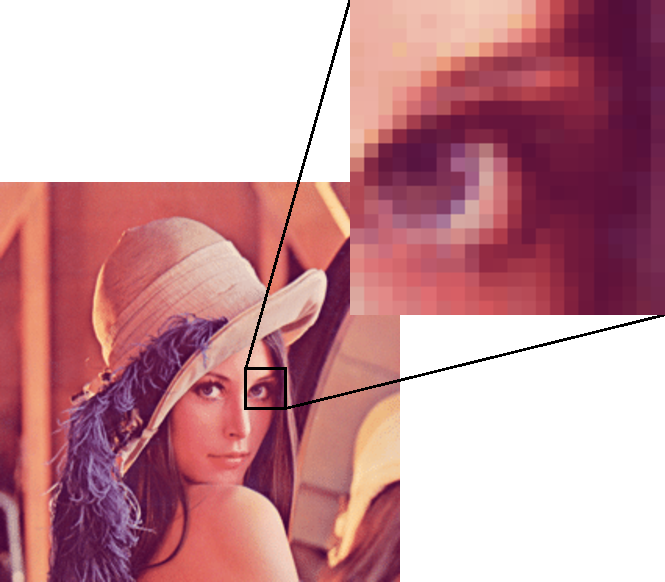
\includegraphics[width=0.5\textwidth]{images/lenaeye.pdf}
  \caption{Lena - detalhe.}\label{fig-lena-detalhe}
  \end{figure}

\end{frame} 

\begin{frame}%[allowframebreaks]
  \frametitle{Espaço necessário para armazenar uma foto}
  \begin{itemize}
  \item câmera 10 Mpixel
  \item 3 bytes por pixel (RGB)
  \item cada foto requer 30 Mbyte
  \item um cartão de memória de 2 Gbytes é capaz de armazenar 66 fotos
  \end{itemize}
\end{frame}

\begin{frame}%[allowframebreaks]
  \frametitle{Espaço necessário para armazenar um vídeo}
  \begin{itemize}
  \item 480 x 720, 30 fps
  \item 345.600 pixels por frame
  \item RGB 3 bytes por pixel
  \item 1.036.800 byte, aprox. 1 Mbyte por frame
  \item 30 frames requerem 31.104.000 bytes, aprox. 31 Mbyte por segundo
  \item um CD de 650 Mbytes é capaz de armazenar apenas 21 segundos de vídeo
  e um DVD de 4.7 GB apenas 155 segundos de vídeo.
  \end{itemize}
\end{frame}


\begin{frame}%[allowframebreaks]
  \frametitle{Dilema de compressão}
  Quando devemos parar a busca por uma \textbf{melhor} compressão?

  \vspace{1cm}
  melhor:
  \begin{itemize}
  \item menor tamanho da representação digital resultante
  \item eficiência computacional (compressão e/ou descompressão)
  \item simplicidade do algoritmo
  \end{itemize}

  \vspace{1cm}
  Qual é o limite de compressão para um determinado dado?

\end{frame} 
\note{
Modificar um algoritmo para melhorar a taxa de compressão em 1\% pode
acarretar um aumento de 10\% no tempo de execução do algoritmo e
ainda mais sobre a complexidade do programa.
}
\note{
Conjecturas\footnote{Uma conjectura é uma proposição que não é provada, mas acredita-se que seja verdadeira e não foi mostrado o contrário.}.
\vspace{2ex}

  \begin{itemize}
  \item Compressão de dados pode ser interpretada como o processo de remover complexidades (redundâncias)
  desnecessárias na informação, e desta forma, maximizando a simplicidade enquanto preserva o máximo
  possível do poder discricionário dos dados.
  \item Todo tipo de computação e racionalização formal pode ser compreendida como compressão
  de informação através do processo de identificar padrões, busca e unificação
  das instâncias destes padrões.
  \end{itemize}

}


\begin{frame}[allowframebreaks]
  \frametitle{Termos}
  \begin{description}
  \item[compressor ou codificador] é o programa que comprime os dados crus na entrada e cria uma saída de dados
  comprimida (com baixa redundância).
  \item[decompressor ou decodificador] converte os dados na direção oposta.
  \item[fluxo] é o dado a ser comprimido, armazenado como um arquivo ou transmitido.
  \item[dado não-codificado, cru, ou original] é o fluxo de dados da entrada.
  \item[dado codificado ou comprimido] é o fluxo de saída.
  \item[método de compressão não-adaptativo] é rígido e não modifica sua operação ou seus parâmetros em resposta
  aos dados em particular que estão sendo comprimidos.
  \item[método adaptativo] analisa os dados crus e modifica sua operação e/ou parâmetros de acordo com os dados em mãos.
  \item[método semi-adaptativo] utiliza 2 passagens aonde, na primeira, realiza a leitura dos dados e
  contabiliza estatísticas dos dados a serem comprimidos; na segunda passagem, realiza de fato a compressão
  utilizados parâmetros determinados na primeira varredura.
  \item[método localmente adaptativo] se adapta às condições locais do fluxo de dados e varia à medida que
  move ao longo dos dados.
  \item[compressão com perdas/sem perdas] : Para atingirem maior compressão, os métodos de compressão com perda
  perdem informação. Os métodos de compressão sem perda não admitem perder informação alguma.
  \item[Compressão em cascata] ocorre quando diferentes métodos de compressão são utilizados um em seguida do outro.
  \item[Compressçao perceptiva] ocorre quando apenas a informação imperceptível pelos nosso sentidos é removida.
  \item[Compressão simétrica] é o caso em que o compressor e descompressor utilizam basicamente o mesmo algoritmo,
  porém em direções opostas.
  \item[Complacente] é o codificador/decodificador que gera/lê de forma correta um fluxo de dados (Qualquer pessoa
  é livre para implementar seu próprio algoritmo).
  \item[Universal] é o método de compressão de dados que não depende da estatística dos dados.
  \item[Razão de Compresão] $=$ tamanho do dado de saída / tamanho do dado de entrada.
  \item[Fator de Compressão] $=$ tamanho do dado de entrada / tamanho do dado de saída $=$ (razão de compressão)$^{-1}$.
  \item[Ganho de Compressão] $= 100 \log_e $ (tamanho de referência / tamanho comprimido), aonde o tamanho de referência é o tamanho dos dados de entrada ou o tamanho do dado de saída comprimido por algum algoritmo padrão.
  \item[Erro médio quadrático (MSE) e relação sinal ruído de sinal (PSNR)] são utilizados para medir a distorção causada por uma compressão com perdas.
  \end{description}
\end{frame} 


\begin{frame}%[allowframebreaks]
  \frametitle{Termos}
  \begin{figure}[h]
  \centering
  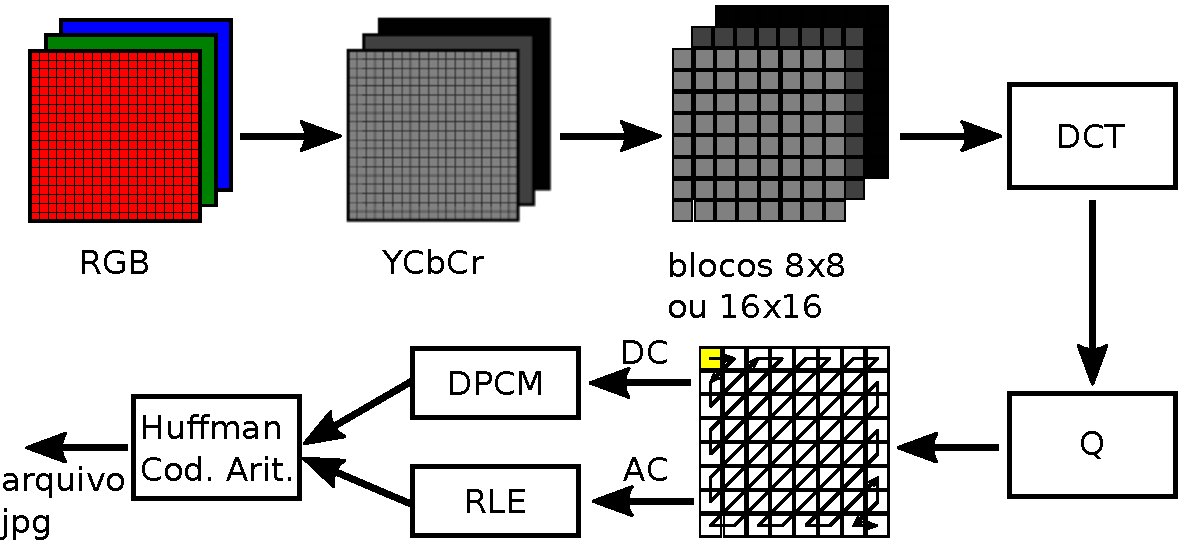
\includegraphics[width=0.8\textwidth]{images/jpegstd.pdf}
  \caption{Esquema de compressão JPEG.}\label{fig-jpegstd}
  \end{figure}
\end{frame} 

\begin{frame}%[allowframebreaks]
  \frametitle{Slides- introdução ao GNU Octave}
  \centering
  
\includegraphics[width=0.4\textwidth]{images/qrcode-octave-intro.pdf}

  \url{https://drive.google.com/open?id=1ew5fl9v_OIybsy3KdEgIvohLTcuwuru_}
\end{frame} 

\begin{frame}%[allowframebreaks]
  \frametitle{Notebook - introdução}
  \centering
  
\includegraphics[width=0.4\textwidth]{images/qrcode-jupyter-intro.pdf}

  \url{https://nbviewer.jupyter.org/github/leolca/notebooks/blob/master/aev/introducao.ipynb}
\end{frame} 

\begin{frame}%[allowframebreaks]
  \frametitle{Notebook - imagem colorida}
  \centering
  
\includegraphics[width=0.4\textwidth]{images/qrcode-jupyter-im-color.pdf}

  \url{https://nbviewer.jupyter.org/github/leolca/notebooks/blob/master/aev/introdocao_imagem_colorida.ipynb}
\end{frame} 



\section{Tecnicas Básicas de Compressão}

\begin{frame}%[allowframebreaks]
  \frametitle{Leitura}
  \centering
  
\includegraphics[width=0.4\textwidth]{images/qrcode-book-salomon.pdf}

  David Salomon, Giovanni Motta - \textit{Handbook of Data Compression}, 2010 \\ 
  \url{https://books.google.com.br/books?id=LHCY4VbiFqAC}\\
  Introduction, Basic Techniques \citep{salomon2010}
\end{frame} 

\subsection{RLE}
\begin{frame}%[allowframebreaks]
  \frametitle{Compressão RLE}
   
  Exemplo:

  string: `2. all is too well'

  codificação: `2. a@2l is t@2o we@2l'

  \vspace{1cm}
  Método MNP5 era utilizado nos modems antigos.

\end{frame}
\note{
MNP : Microcom Networking Protocol

"The MNP5 method is a two-stage process that starts with run-length encoding, followed by adaptive frequency encoding."
\citep{salomon2000}

"With MNP 5, the data received from the computer are first compressed with a simple algorithm, and then passed into the MNP 4 packetizing system for transmission. On best-case data the system offered about 2:1 compression, but in general terms about 1.6:1 was typical, at least on text. As a result a 2400 bit/s modem would appear to transfer text at ~4000 bit/s, even though the modem was still running at the same 600 baud * 4 bits per symbol rate.

This dramatic increase in throughput allowed Microcom modems to remain somewhat competitive with models from other companies that were otherwise nominally much faster. For instance, Microcom generally produced 1200 and 2400 bit/s modems using commodity parts, while companies like USRobotics and Telebit offered models with speeds up to 19200 bit/s."
(\url{https://en.wikipedia.org/wiki/Microcom_Networking_Protocol})
}


\begin{frame}%[allowframebreaks]
  \frametitle{Compressão RLE}
 
  Exemplo: uma imagem em tons de cinza com 8-bit de profundidade começa com os seguintes valores

  12, 12, 12, 12, 12, 12, 12, 12, 12, 35, 76, 112, 67, 87, 87, 87, 5, 5, 5, 5, 5, 5, 1, ...

  será comprimida como  \framebox{9},12,35,76,112,67,\framebox{3},87,\framebox{6},5,1, ...

  \vspace{1cm}
  Se utilizarmos como \textit{flag} o valor 255, então a sequência acima será expressa por

  255, 9, 12, 35, 76, 112, 67, 255, 3, 87, 255, 6, 5, 1, ...

  \vspace{1cm}
  grupos de 8

  \framebox{10000010},9,12,35,76,112,67,3,87,\framebox{100...},6,5,1, ...

\end{frame} 

\begin{frame}%[allowframebreaks]
  \frametitle{Exemplo RLE - GNU Octave}
  \centering
  
\includegraphics[width=0.4\textwidth]{images/qrcode-jupyter-rle.pdf}

  \url{https://nbviewer.jupyter.org/github/leolca/notebooks/blob/master/aev/rle_mario.ipynb}
\end{frame} 


\begin{frame}%[allowframebreaks]
  \frametitle{Move-to-Front Coding}
  Consideramos o alfabeto de símbolos $\mathcal{A}$ como uma lista 
  onde os símbolos mais frequentes estarão dispostos no início da lista.

  O método é localmente adaptativo, já que ele se adapta à frequência dos
  símbolos em cada região do fluxo de dados.
\end{frame} 


\begin{frame}%[allowframebreaks]
  \frametitle{Move-to-Front Coding - Exemplo \citep{salomon2010}}

   Exemplo:
   entrada a ser codificada: \textbf{abcddcbamnopponm}

  \begin{columns}[c]
  \column{.4\textwidth}
  C = (0, 1, 2, 3, 0, 1, 2, 3, 4, 5, 6, 7, 0, 1, 2, 3) \\
  -- utilizando move-to-front\\
  \vspace{1cm}
  C' = (0, 1, 2, 3, 3, 2, 1, 0, 4, 5, 6, 7, 7, 6, 5, 4) \\
  -- sem utilizar move-to-front 
  \column{.6\textwidth}
     \vspace{-0.2cm}
     \begin{figure}[h!]
     \centering
     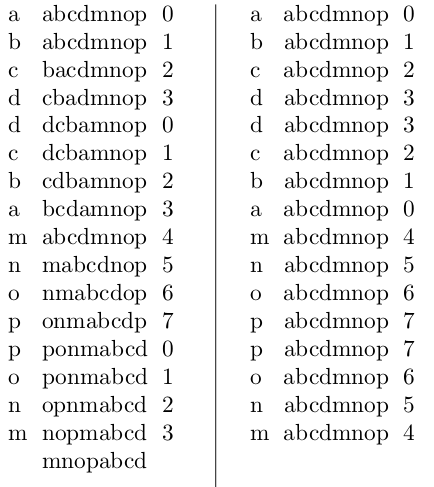
\includegraphics[width=0.7\textwidth]{images/move_to_front_coding.png}
     %\caption{}
     \label{fig:move_to_front_coding}
     \end{figure}
  \end{columns}

\end{frame} 

\begin{frame}%[allowframebreaks]
  \frametitle{Move-to-Front Coding - Exemplo \citep{salomon2010}}
  \begin{columns}[c]
  \column{.4\textwidth}
  O resultado $C$ obtido pelo move-to-front é tal que, na média, os valores
  em $C$ são pequenos (os valores no início do dicionário são os mais prováveis).
  Isto faz com que a saída seja propícia para ser codificada através da codificação
  de Huffman ou codificação aritmética.
  \column{.4\textwidth}
     \begin{figure}[h!]
     \centering
     \includegraphics[width=0.65\textwidth]{/home/leoca/ee/ufsj/2012_01/audio_video/aulas/images/variable_sized_codes.png}
     \caption{Exemplo de código de tamanho variável.}
     \label{fig:variable_sized_codes}
     \end{figure}
  \end{columns}

\end{frame}


\begin{frame}%[allowframebreaks]
  \frametitle{Move-to-Front Coding}
  Variações:
  \begin{enumerate}
  \item Move-ahead-k: O elemento do alfabeto A que corresponde ao símbolo corrente será deslocado k posições para cima na lista ao
          invés de ir para o topo da lista.
  \item Wait-c-and-move: O elemento do alfabeto A será deslocado para o início da lista apenas após aparecer c vezes durante a
          codificação. 
  item Wait-c-and-ahead-k: Um combinação das duas variantes anteriores.
  \end{enumerate}

\end{frame} 

\begin{frame}%[allowframebreaks]
  \frametitle{Exemplo Move-to-Front - GNU Octave}
  \centering
  
\includegraphics[width=0.4\textwidth]{images/qrcode-jupyter-m2f.pdf}

  \url{https://nbviewer.jupyter.org/github/leolca/notebooks/blob/master/aev/move-to-front.ipynb}
\end{frame} 





% quantização escalar
\section{Quantização Escalar}
\subsection{Conversão AD/DA}
\begin{frame}%[allowframebreaks]
  \frametitle{Conversão AD/DA}

  \begin{figure}[h]
  \centering
  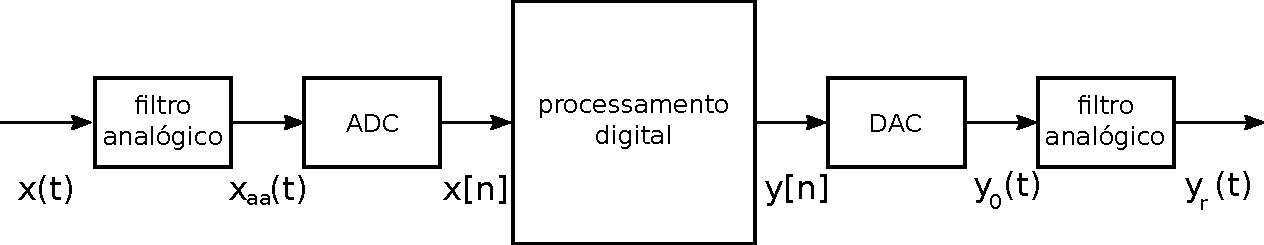
\includegraphics[width=0.7\textwidth]{images/conversaoadda.pdf}
  \caption{Processamento digital de sinais. Conversão AD e DA.}\label{fig-conv-adda}
  \end{figure}

\end{frame}


\begin{frame}%[allowframebreaks]
  \frametitle{Quantização}

  \begin{figure}[h]
  \centering
  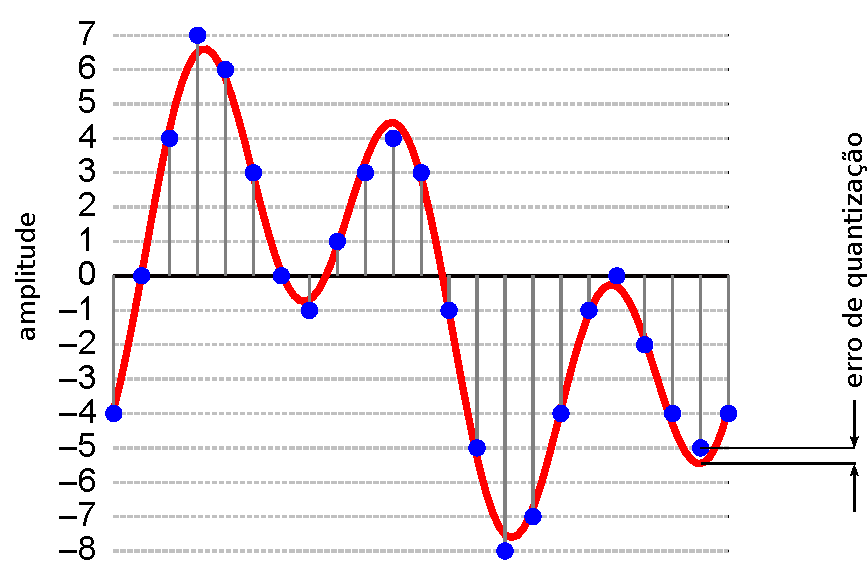
\includegraphics[width=0.5\textwidth]{images/digitalization.pdf}
  \caption{Quantização.}\label{fig-sig-quantz}
  \end{figure}

\end{frame}

\begin{frame}%[allowframebreaks]
  \frametitle{Amostragem}
  Ao amostrar um sinal $x(t)$ com período de amostragem $T_s$ teremos
  \begin{eqnarray}
  x_s(t) &=& x(t) s(t) \nonumber \\ 
        &=& x(t) \sum_{k=-\infty}^{\infty} \delta(t - kT_s) \nonumber \\
         &=& \sum_{k=-\infty}^{\infty} x(kT_s) \delta(t - kT_s)
  \end{eqnarray}

\end{frame}


\begin{frame}%[allowframebreaks]
  \frametitle{Amostragem}

  \begin{figure}[h]
  \centering
  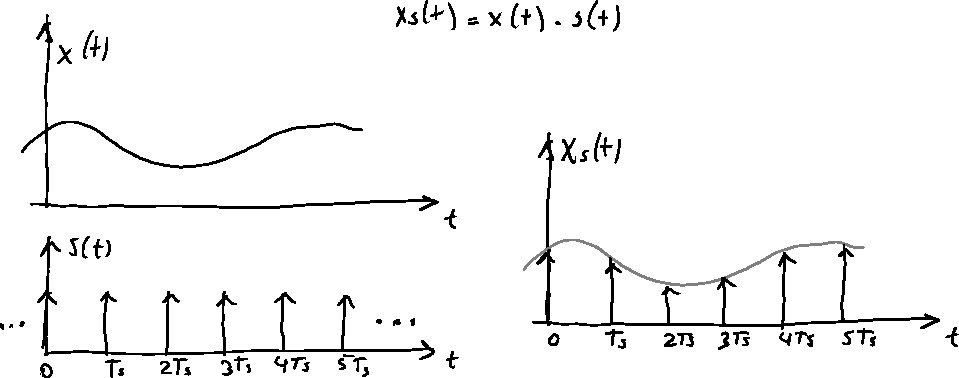
\includegraphics[width=0.8\textwidth]{images/amostragem.pdf}
  %\caption{.}
  \label{fig-amostragem}
  \end{figure}

\end{frame}

\begin{frame}[allowframebreaks]
  \frametitle{Amostragem}
  Como $s(t) = \sum_{k=-\infty}^{\infty} \delta(t - kT_s)$ é periódico com período $T_s$,
  podemos representá-lo por uma série de Fourier:
  \begin{equation}
  s(t) = \sum_{k=\infty}^{\infty} \delta(t - kT_s) = \sum_{k=-\infty}^{\infty} c_k e^{j 2 \pi t k /T_s} \textmd{,}
  \end{equation}
  onde
  \begin{equation}
  c_k = \frac{1}{T_s} \int_{-T_s/2}^{T_s/2} \delta(t) e^{-j2\pi t k/T_s} dt = \frac{1}{T_s}
  \end{equation}
  Desta forma, $x_s(t) = x(t) \cdot s(t)$ poderá ser expresso por
  \begin{equation}
  x_s(t) = \frac{1}{T_s} \sum_{k=-\infty}^{\infty} x(t) e^{j2\pi tk /T_s} \textmd{.}
  \end{equation}

  A multiplicação por $\exp(j 2\pi \alpha t)$ corresponde, na frequência, a um deslocamento de $\alpha$. 
  Teremos assim
  \begin{equation}\label{eq-Xs-freqdom}
  X_s(j \Omega) = \frac{1}{T_s} \sum_{k=-\infty}^{\infty} X \left( j (\Omega - n \Omega_s) \right)
  \end{equation}

  
  \framebreak

  Podemos chegar ao mesmo resultado sabendo que, se no domínio do tempo temos $x_s(t) = x(t) \cdot s(t)$, 
  no domínio da frequência temos
  \begin{equation}\label{eq-conv-dom-freq}
  X_s(j \Omega) = \frac{1}{2\pi} X(j \Omega) \ast S(j \Omega) .
  \end{equation} 
  Como a transformada de Fourier de $s(t)$ é
  \begin{equation}\label{eq-pulse-train-freq}
  S(j \Omega) = \frac{2\pi}{T_s} \sum_{k=-\infty}^{\infty} \delta(\Omega - k \Omega_s) ,
  \end{equation}
  onde $\Omega_s = \nicefrac{2\pi}{T}$, então utilizando as \Cref{eq-conv-dom-freq,eq-pulse-train-freq} obtemos \Cref{eq-Xs-freqdom}.

  \framebreak

  Se $x(t)$ for um sinal limitado em frequência ($\Omega_N$ frequência máxima) e
  não havendo \textit{aliasing}, $\Omega_s > 2 \Omega_N$, podemos reconstruir $x(t)$:
  \begin{equation}\label{eq-x-reconstruido}
  X_r(j \Omega) = H_r(j \Omega) X_s(j \Omega)
  \end{equation}
  onde $H_r$ é um filtro passa-baixas ideal com $\Omega_N < \Omega_c < \Omega_s$.

  \begin{equation}
  H_r (j \Omega) = \begin{cases}1 \quad & \textmd{, se \ \ } \vert \Omega \vert \leq \Omega_c,\\ 0 & \mbox{, caso contrário.}\end{cases}
  \end{equation}

  \vspace{2ex}
  (Teorema da Amostragem)

  \vspace{3ex}
  Leitura: Capítulo 4 \bibentry{oppenheim2009}.
\end{frame}



\begin{frame}%[allowframebreaks]
  \frametitle{Amostragem}

  \begin{figure}[h]
  \centering
  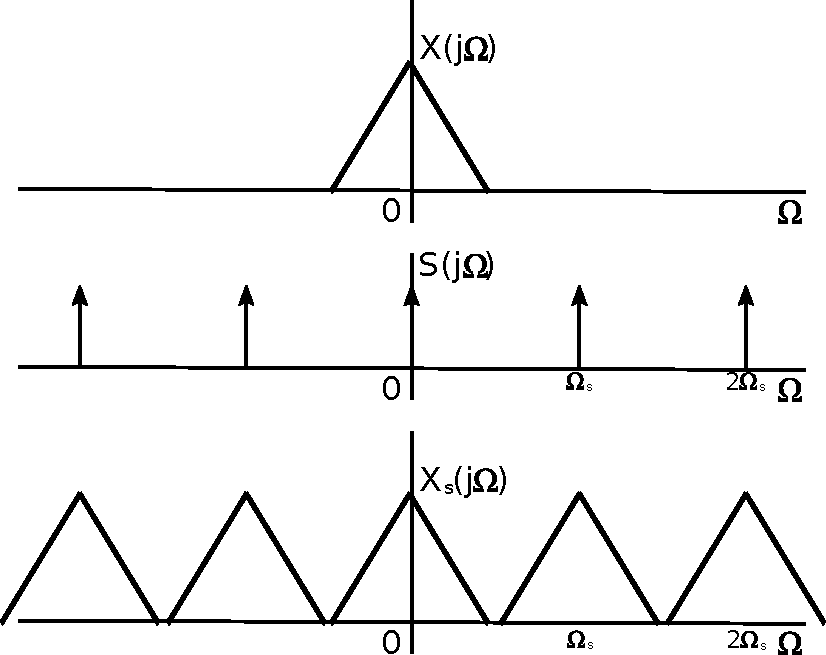
\includegraphics[width=0.6\textwidth]{images/sampling-freq-a.pdf}
  %\caption{.}
  \label{fig-sampling-freq-a}
  \end{figure}

\end{frame}

\begin{frame}%[allowframebreaks]
  \frametitle{Amostragem}

  \begin{figure}[h]
  \centering
  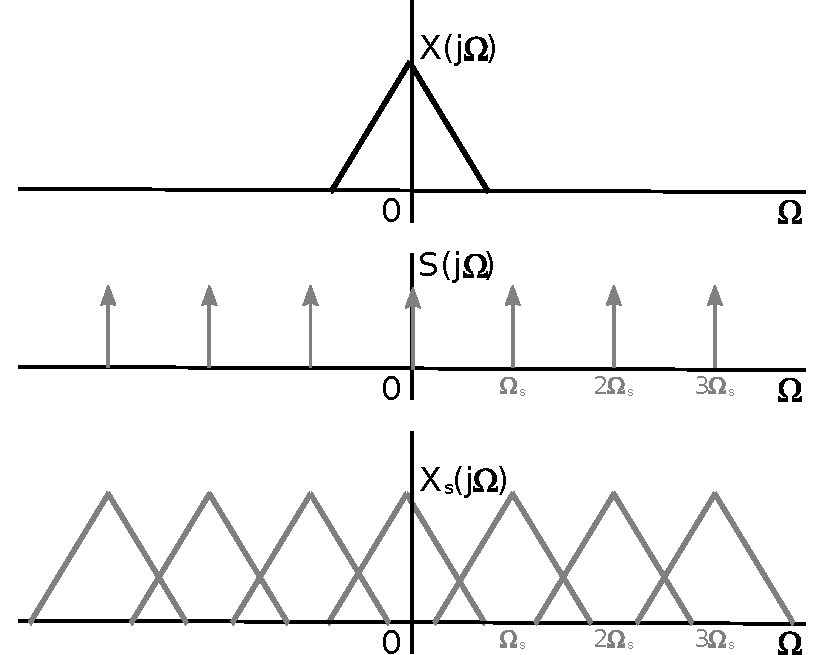
\includegraphics[width=0.6\textwidth]{images/sampling-freq-b.pdf}
  %\caption{.}
  \label{fig-sampling-freq-a}
  \end{figure}

\end{frame}


\subsection{Quantização Escalar}
\begin{frame}[allowframebreaks]
  \frametitle{Quantização Escalar}

  Quantização escalar é um mapeamento $Q$ de valores reais $x$ de uma variável aleatória
  contínua $X$ nos valores $y = Q(x)$, mais próximos de $x$ (em termos de uma determinada medida de distorção),
  de um conjunto discreto e finito $Y = {y_1 , y_2 , \ldots,  y_M }$.
  Os valores $y_i$ , $i = 1, 2, \ldots , M$, são chamados níveis de saída, ou valores de representação,
  ou ainda valores de aproximação. $Y$ é chamado de \textit{codebook} ou conjunto de aproximação.

  \framebreak

  O quantizador escalar é determinado pelo conjunto de limiares 
  $\mathcal{T} = \{t_i\}$, $i=0, 1, \ldots, M$
  e pelo conjunto de pontos de representação $\mathcal{Y} = \{y_i\}$, $i=1, \ldots, M$. 
  Os limiares dividem exaustivamente o domínio $\mathit{R}$ em subintervalos 
  (ou células, regiões de representação) $\Delta_i = (t_{i-1} , t_i ]$ disjuntas,
  ou seja, $\Delta_i \cap \Delta_j = \emptyset$. Diz-se que a divisão é exaustiva
  pois $\bigcup_{i=1}^M \Delta_i = \mathit{R}$. Esta divisão é tal que existe apenas
  um $y_i$ associado a cada intervalo $\Delta_i$, ou seja, $y_i = Q(x)$ se e somente se
  $x \in \Delta_i$. 

  \framebreak 

  \begin{figure}[h!]
  \centering
  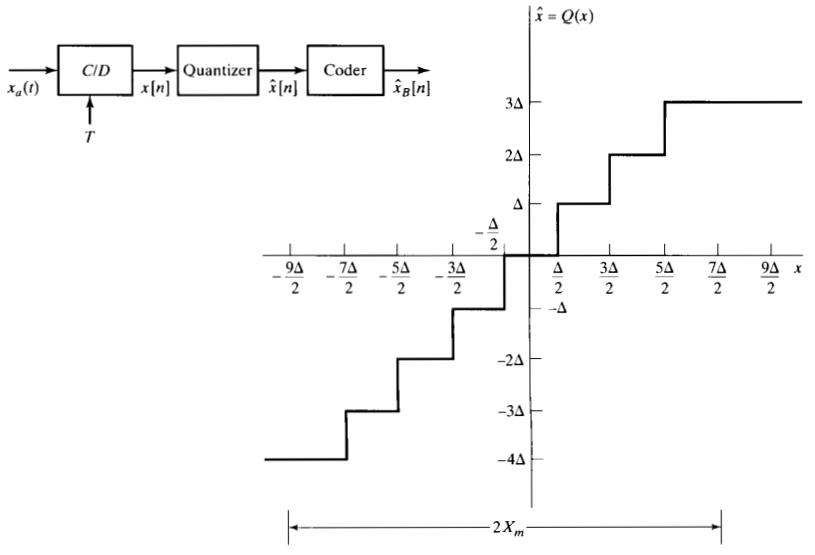
\includegraphics[width=0.6\textwidth]{images/quantization-oppenheim-fig447.png}
  \caption{Quantização. Fonte: \cite{oppenheim2009}.}
  \label{fig:quantization-fig447}
  \end{figure}  

  \framebreak

  É inerente ao processo de quantização a introdução de um erro, chamado \textit{erro de quantização}
  ou \textit{ruído de quantização}.

  O erro de quantização esperado é dado por
  \begin{equation}
  D(Q) = E\left\lbrace d(x,Q(x)) \right\rbrace ,
  \end{equation}
  onde $d(x,Q(x))$ é uma medida de distorção entre $x$ e $Q(x)$, dada por $d(\cdot)$.

  A taxa de quantização é o número de bits $R$ que é utilizado na representação de um valor $x$.
  Ela é dada em bits por amostra.

  Para um quantizador com taxa fixa temos $R = \log_2 M$ bits por amostra.

  \framebreak

  \begin{figure}[h!]
  \centering
  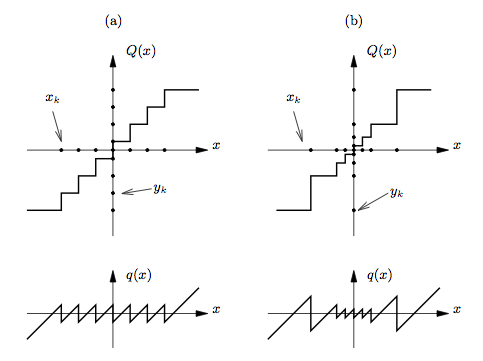
\includegraphics[width=0.55\textwidth]{/home/leoca/ee/ufsj/2012_01/audio_video/aulas/images/quantizationerror.png}
  \caption{(a) linear (b) logarítmico. Fonte: \cite{oppenheim2009}.}
  \label{fig:quantizationerror}
  \end{figure}  

\end{frame}

\subsection{Entropia na saída do quantizador}
\begin{frame}[allowframebreaks]
  \frametitle{Entropia na saída do quantizador}
  As probabilidades dos níveis de representação de um quantizador podem ser determinadas,
  conhecendo-se a pdf do sinal.

  Seja $f(x)$ a pdf (função densidade de probabilidade) de $X$. Podemos calcular a probabilidade
  do i-ésimo nível de reprodução (a probabilidade de $x \in \Delta_i$) como
  \begin{equation}
  P(y_i) = \int_{t_i -1}^{t_i} f(x) \mathrm{d}x .
  \end{equation}
  A entropia da saída do quantizador é igual a
  \begin{equation}
  H(Y) = - \sum_{i=1}^{M} P(y_i) \log_2 P(y_i) .
  \end{equation}

  Um código de comprimento variável poder ser utilizado para representar a saída 
  do quantizador (exemplo: código de Shannon, código Huffman, ou codificação aritmética).
\end{frame}
\note{
Shannon: o limite de representação é a entropia.

O limite para se representar um sinal, sem perdas, será dado pela entropia da fonte.
}


\subsection{Quantização Escalar Uniforme}
\begin{frame}[allowframebreaks]
   \frametitle{Quantização escalar uniforme}
  A quantização escalar é uniforme quando os limiares estão igualmente espaçados,
  e desta forma, as células possuem o mesmo tamanho (exceto as extremas, primeira e última),
  ou seja, $\vert \Delta_i \vert = \delta$, e o ponto de representação localiza-se no 
  ponto médio da célula,
  \begin{equation}
  y_i = \frac{t_{i-1} + t_i}{2} = t_{i-1} + \frac{\delta}{2} , \ \ i=1,2,\ldots,M .
  \end{equation}

  \framebreak

  (*obs.: considerando apenas valores positivos)

  Dada a entrada $x$, a célula associada a $x$ é determinada por
  \begin{equation}
  i = [x / \delta ] ,
  \end{equation}
  onde $\delta$ é a largura de cada célula e $[ \cdot ]$ representa a operação
  de arredondamento.
 
  O valor de aproximação para a entrada $x$ é dado por
  \begin{equation}
  y = Q(x) = \delta \left[ \frac{x}{\delta} \right]   
  \end{equation}
  isto é, a i-ésima célula é determinada por $\Delta_i = (i\delta - \delta/2, i\delta + \delta/2]$
  e $y_i = i\delta$.

\end{frame}

\begin{frame}%[allowframebreaks]
   \frametitle{Distorção no quantizador escalar uniforme}
  Se $f(x)$ é conhecida, então podemos calcular a distorção esperada do quantizador
  \begin{equation}
  D(Q) = \int_{-\infty}^{\infty} f(x) d(x,Q(x)) dx = \sum_i \int_{t_{i-1}}^{t_i} f(x) d(x,y_i) \mathrm{d}x .
  \end{equation}

  Se o erro de distorção é medido pelo erro quadrático, então $D(Q)$ fornecerá o 
  erro quadrático médio (MSE, \textit{Mean Squared Error}):
  \begin{equation}
  D(Q) = \sum_i \int_{t_{i-1}}^{t_i} f(x) (x - y_i)^2 \mathrm{d}x .
  \end{equation}
\end{frame}




\subsection{Quantização Escalar Não-Uniforme}

\begin{frame}[allowframebreaks]
   \frametitle{Quantização escalar não-uniforme}
 
  Se conhecemos as características estatísticas de $X$, podemos utilizar esta informação
  para melhorar as características do quantizador.

  \begin{figure}[h!]
  \centering
  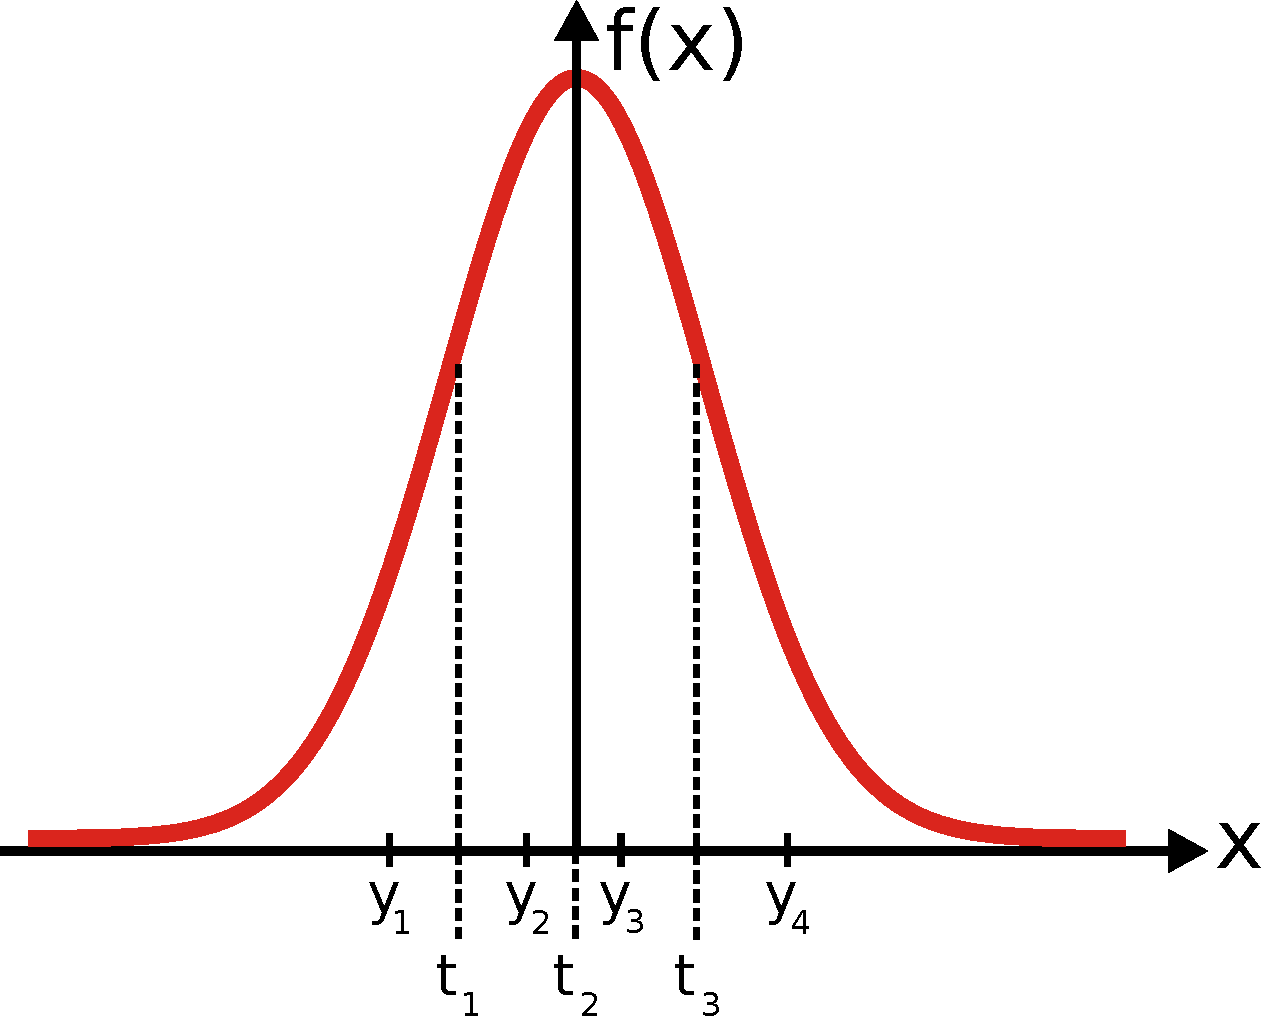
\includegraphics[width=0.45\textwidth]{images/quantz-gaussian.pdf}
  %\caption{}
  \label{fig:quantz-gaussian}
  \end{figure}  
\end{frame}



\subsection{Lloyd-Max}
\begin{frame}[allowframebreaks]
  \frametitle{Algoritmo de Lloyd-Max}
  O algoritmo de \emph{Lloyd-Max} é um algoritmo para encontrar os limiares $\{t_i\}$ e
  os pontos de representação $\{y_i\}$ que minimizam a distorção.

  Lloyd e Max criaram um procedimento para construir uma solução para o problema, que satisfaz
  as condições necessárias (mas não suficientes):

  \begin{itemize}
  \item os limiares devem ficar entre os pontos de representação:
        \begin{equation}
        t_i = \frac{y_{i+1} + y_{i}}{2} \quad , 1 \leq i \leq M-1 , 
        \end{equation}
  \item os pontos de representação devem ficar no meio (com relação à esperança) de um dado intervalo
        \begin{equation}
        y_i = E [ X(i) ] = \frac{ \int_{t_{i-1}}^{t_i} x f_X (x) dx }{ \int_{t_{i-1}}^{t_i} f_X (x) dx  } .
        \end{equation}
  \end{itemize}

  \framebreak
  Algoritmo:
  \begin{enumerate}
  \item Escolher um conjunto inicial arbitrário com $M$ pontos de representação $y_1 < y_2 < \ldots y_M$.
  \item Para cada $i$, $1 \leq j \leq M-1$, fazer $t_i = \frac{1}{2} (y_{i+1} + y_i)$.
  \item Para cada $i$, $1 \leq j \leq M-1$, fazer $y_i$ igual à média condicional de $X \sim f(x)$,
        dado $X \in (t_{i-1}, t_i]$ (onde $t_0$ e $t_M$ são respectivamente $-\infty$ e $+\infty$).
  \item Repetir os passos (2) e (3) até que a melhoria no MSE seja desprezível; então interromper.
  \end{enumerate}
  O MSE decresce (ou permanece o mesmo) a cada passo do algoritmo. Como o MSE é não-negativo,
  ele irá se aproximar de um limite em um número finito de passos, pois o algoritmo será interrompido
  quando a melhoria no MSE foi menor que um dado $\epsilon > 0$.

  \framebreak
  O exemplo abaixo ilustra que o algoritmo deve chegar a um mínimo local.
  Considere $M=2$ pontos de representação e uma pdf $f(x)$ como definida na Figura \ref{fig:lloyd-ex}.

  \begin{figure}[h!]
  \centering
  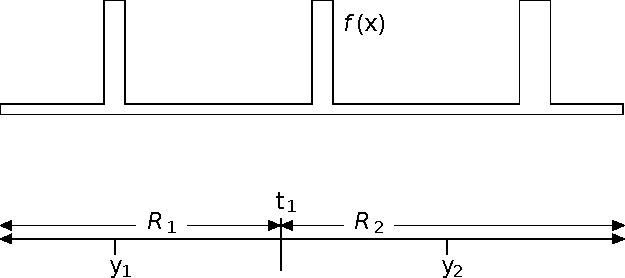
\includegraphics[width=0.55\textwidth]{images/lloyd-ex.pdf}
  \caption{Exemplo Lloyd-Max: regiões e pontos de representação que satisfazem 
        a condição de parada do algoritmo nas não minimizam a distorção média quadrática.
	Fonte: \citet{gallager2008}}
  \label{fig:lloyd-ex}
  \end{figure}

  \framebreak

  A configuração apresentada na Figura \ref{fig:lloyd-ex} satisfaz os critérios de parada, entretanto
  o pico mais a direita é mais provável que os outros dois, desta forma, o MSE poderia ser menor se 
  $R_1$ cobrisse a regiões dos dois picos à esquerda e $R_2$ apenas o pico à direita.

  \vspace{2ex}
  Leitura: Capítulo 3 \bibentry{gallager2008}.
\end{frame}







\subsection{Performance do Quantizador}

\begin{frame}[allowframebreaks]
  \frametitle{Performance do Quantizador}
  Seja $p(x)$ a pdf do sinal de entrada $x$, então o erro médio quadrático (MSE) 
  devido à quantização será dado por
  \begin{equation} \label{eq-sqnr-quants}
  \sigma_q^2 = \sum_{k=1}^{M} \int_{t_{k-1}}^{t_k} (x - y_k)^2 p(x) \mathrm{d}x.
  \end{equation}

  Se $M$ for grande e a pdf $p(x)$ for suave, poderemos aproximar $p(x)$ no intervalo $(t_{k-1},t_{k}]$ como
  \begin{equation}
  p(x) \approx p\left(\frac{t_{k-1}+t_{k}}{2}\right) , \quad t_{k-1} < x \leq t_k ,
  \end{equation}
  e assim, a equação \ref{eq-sqnr-quants} poderá ser reescrita como
  \begin{equation} \label{eq-sqnr-quants2}
  \sigma_q^2 = \sum_{k=1}^{M} p\left(\frac{t_{k-1}+t_{k}}{2}\right) \int_{t_{k-1}}^{t_k} (x - y_k)^2 \mathrm{d}x.
  \end{equation}

  Mostra-se que
  \begin{equation} \label{eq-sqnr-int}
  \int_{t_{k-1}}^{t_k} (x - y_k)^2 \mathrm{d}x = \Delta_k \left[ \left( y_k - \frac{t_{k-1} + t_{k}}{2} \right)^2 + \frac{\Delta_k^2}{12} \right] ,
  \end{equation}
  onde $\Delta_k = t_k - t_{k-1}$ é o tamanho do passo do quantizador.

  Para minimizar o MSE devemos escolher $y_k = (t_{k-1} + t_{k})/2$, 
  de forma que o primeiro termo em \ref{eq-sqnr-int} se anule. Ou seja,
  devemos escolher os pontos de representação como o ponto médio dos limiares dos intervalos.
  (obs.: Isto ocorre devido à aproximação feita para $p$ suave e $M$ grande. No caso geral,
  deveremos ter os pontos de representação no valor esperado de cada intervalo)

  Vamos definir $p_k$ como a probabilidade de $x$ pertencer ao intervalo $(t_{k-1},t_k]$.
  Usando a aproximação feita anteriormente, teremos
  \begin{equation} \label{eq-pk-aprox}
  p_k = \Pr(t_{k-1} < x \leq t_k) \approx p\left(\frac{t_{k-1}+t_{k}}{2}\right) \Delta_k ,
  \end{equation}
  e assim podemos reescrever a equação \ref{eq-sqnr-quants2} como
  \begin{equation} \label{eq-sqnr-quants3}
  \sigma_q^2 = \frac{1}{12} \sum_{k=1}^{M} p_k \Delta_k^2 .
  \end{equation}

\end{frame}


\subsection{Quantizador Uniforme}
\begin{frame}[allowframebreaks]
  \frametitle{Performance do Quantizador Uniforme} 

  Para o quantizador uniforme o passo é constante ($\Delta_k = \Delta$ para todo $k$). Teremos assim
  \begin{equation} \label{eq-sqnr-quants-uni}
  \sigma_q^2 = \frac{\Delta^2}{12} \underbrace{ \sum_{k=1}^{M} p_k }_{=1} = \frac{\Delta^2}{12} .
  \end{equation}
  Note que a potência do ruído de quantização é independente da distribuição do sinal.

  A performance do quantizador será expressa pela relação sinal-ruído de quantização (SQNR),
  \begin{equation} \label{eq-sqnr-unif}
  \textmd{SQNR} = 10 \log \left( \frac{\sigma_x^2}{\sigma_q^2} \right) = 10 \log \left( \frac{12 \sigma_x^2}{\Delta^2} \right) \mathrm{dB}.
  \end{equation}
\end{frame}

\begin{frame}[allowframebreaks]
  \frametitle{Performance do Quantizador Uniforme - Sinal Senoidal}
  Vamos supor que o sinal de entrada seja da forma $A \sin \omega t$ e 
  um quantizador uniforme com $n$ bits ($2^n = M$). Podemos escolher $\Delta$
  para que não ocorra saturação. Faremos então $\Delta = A/2^{n-1}$.
  A potência do sinal senoidal é $\sigma_x^2 = A^2/2$. Usando agora a Equação \ref{eq-sqnr-unif}, teremos
  \begin{equation} \label{eq-sqnr-unif-sin}
  \textmd{SQNR (senoide)}  = 6n + 1.76 \mathrm{dB}.
  \end{equation}
\end{frame}

\begin{frame}[allowframebreaks]
  \frametitle{Performance do Quantizador Uniforme - Sinal Gaussiano}
  Iremos supor agora um sinal de entrada com distribuição gaussiana: $p(x)=1/\sqrt{2\pi\sigma} e^{-(x^2/2\sigma^2)}$.
  Para que a distorção por saturação seja desprezível, iremos fazer $2^{n-1} \Delta = 4 \sigma$, ou seja, teremos $\Delta = \sigma/2^{n-3}$.
  A potência média quadrática do sinal de entrada é $\sigma_x^2 = \sigma^2$. Usando agora a Equação \ref{eq-sqnr-unif}, teremos
  \begin{equation} \label{eq-sqnr-unif-gaus}
  \textmd{SQNR (gauss)}  = 6n - 7.3 \mathrm{dB}.
  \end{equation}
\end{frame}


\subsection{Quantizador Não Uniforme}
\begin{frame}%[allowframebreaks]
  \frametitle{Quantizador Não Uniforme}

  Os sinais de fala, por exemplo, estão geralmente concentrados em torno da origem.
  Desta forma, seria interessante propor um quantizador em que os passos de quantização
  fossem menores na região de menor amplitude do sinal e maiores na região de maior amplitude.
  Isto levaria a uma redução do ruído de quantização total.

  \begin{figure}[h!]
  \centering
  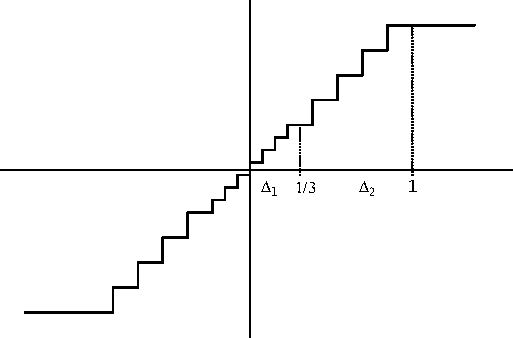
\includegraphics[width=0.4\textwidth]{images/nuquantz.pdf}
  \caption{Exemplo de quantizador não uniforme de 4 bits, com $\Delta_1 = \Delta_2/2$ \citep{tokunbo}.}
  \label{fig:nuquantz}
  \end{figure}
\end{frame}


\subsection{Compressor e Expansor}
\begin{frame}%[allowframebreaks]
  \frametitle{Compressor e Expansor}
  Podemos utilizar compressor e expansor para implementar um quantizador não uniforme.

  \begin{description}
  \item[compressor] é feito para amplificar os sinais de baixa amplitude, às custas de atenuar os sinais de alta amplitude;
  \item[expansor] faz o inverso.
  \end{description}

  \begin{figure}[h!]
  \centering
  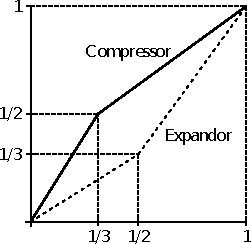
\includegraphics[width=0.3\textwidth]{images/compressor.pdf}
  \caption{Exemplo de compressor e expansor \citep{tokunbo}.}
  \label{fig:compressor}
  \end{figure}
\end{frame}


\begin{frame}[allowframebreaks]
  \frametitle{Performance do Quantizador Não Uniforme}

  O erro médio quadrático devido à quantização é dado pela Equação \ref{eq-sqnr-quants3}, repetida a seguir,
  \begin{equation} 
  \sigma_q^2 = \frac{1}{12} \sum_{k=1}^{M} p_k \Delta_k^2  , \nonumber
  \end{equation}
  onde $p_k = \Pr(t_{k-1} < x \leq t_k)$ e $\Delta_k = (t_k - t_{k-1})$.

  Suponha que o compressor apresentado na Figura \ref{fig:excompressor} seja utilizado.
  \begin{figure}[h!]
  \centering
  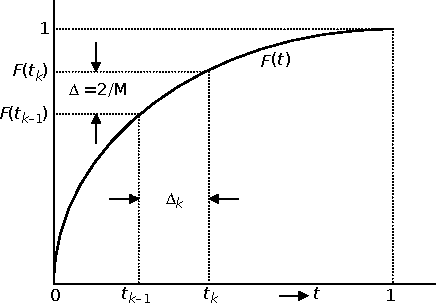
\includegraphics[width=0.6\textwidth]{images/excompressor.pdf}
  \caption{Exemplo de compressor \citep{tokunbo}.}
  \label{fig:excompressor}
  \end{figure}

  Os limiares $t_{k-1}$ e $t_{k}$, correspondentes a um codificador não uniforme, são mapeados 
  através da função compressora $F(\cdot)$ nos limiares $F(t_{k-1})$ e $F(t_k)$, uniformemente espaçados.
  Supondo o sinal no intervalo $[-1,+1]$, teremos $\Delta = 2/M$, o passo do codificador uniforme.
  Conhecendo $\Delta$ e a derivada (inclinação) de $F(t)$ no intervalo $[t_{k-1},t_{k}]$, podemos 
  determinar $\Delta_k$,
  \begin{equation}\label{eq-dk-F}
  \Delta_k = \frac{\Delta}{F'(t_k^{\ast})} = \frac{2}{M F'(t_k^{\ast})}, \quad t_{k-1} < t_k^\ast < t_k .
  \end{equation} 

  Substituindo $\Delta_k$ na Equação \ref{eq-sqnr-quants3}, teremos
  \begin{equation} \label{eq-sqnr-q-nu}
  \sigma_q^2 = \frac{1}{3} \sum_{k=1}^{M} \frac{p_k}{M^2 (F'(t_k^{\ast}))^2} , \quad t_{k-1} < t_k^\ast < t_k .
  \end{equation}

  Se o número de níveis $M$ for grande, o somatório em \ref{eq-sqnr-q-nu} poderá ser aproximado por
  uma integral:
  \begin{equation} \label{eq-sqnr-q-nu2}
  \sigma_q^2 = \frac{1}{3M^2} \int_{-1}^{+1} \frac{p(x)}{ (F'(x))^2 } \mathrm{d}x = \frac{2}{3M^2} \int_{0}^{+1} \frac{p(x)}{ (F'(x))^2 } \mathrm{d}x  ,
  \end{equation}
  onde utilizamos a simplificação em que a $p(x)$ é simétrico par.

  Para um sinal com excursão entre $-X_m$ e $+X_m$, teremos
  \begin{equation} \label{eq-sqnr-q-nu2}
  \sigma_q^2 = \frac{2 X_m^2}{3M^2} \int_{0}^{X_m} \frac{p(x)}{ (F'(x))^2 } \mathrm{d}x  .
  \end{equation} 

\end{frame}

\begin{frame}[allowframebreaks]
  \frametitle{Compressão Logarítmica}
  Em um sistema de telecomunicações, desejamos uma SNR constante, independente da distribuição do sinal de entrada.
  Desejamos então encontrar o compressor $F$ que alcança este objetivo.

  \begin{equation} \label{eq-sqnr-log-const}
  \textmd{SNR} = \frac{\sigma_x^2}{\sigma_q^2} = \frac{2 \int_0^1 x^2 p(x) \mathrm{d}x}{ \frac{2}{3M^2} \int_0^1 \frac{p(x)}{(F'(x))^2} \mathrm{d}x } .
  \end{equation}
  A expressão em \ref{eq-sqnr-log-const} pode ser feita constante escolhendo
  \begin{equation} \label{eq-dcompr}
  F'(x) = \frac{k^{-1}}{x} ,
  \end{equation}
  com parâmetro $k$ a ser especificado.

  A curva de compressão $F(x)$ é obtida realizando-se a integração e escolhendo a constante de integração 
  para que a condição de contorno $F(1)=1$ seja satisfeita, obtendo assim
  \begin{equation} \label{eq-compr}
  F(x) = 1 + k^{-1} \ln x .
  \end{equation}
  Para este caso a SNR obtida será
  \begin{equation} \label{eq-sqnr-log-const2}
  \textmd{SNR} =  \frac{3M^2}{k^2} .
  \end{equation}
  Para sinal com extensão de $-X_m$ a $X_m$, teremos
  \begin{equation} \label{eq-compr2}
  F(x) = X_m + k^{-1} \ln \left(\frac{x}{X_m}\right) .
  \end{equation}

  \begin{figure}[h!]
  \centering
  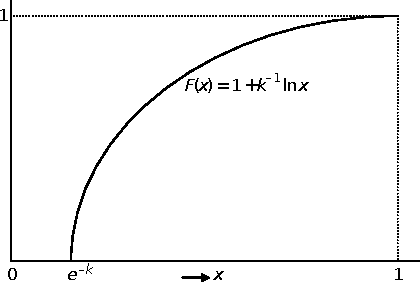
\includegraphics[width=0.6\textwidth]{images/Fx.pdf}
  \caption{Gráfico de $F(x) = 1 + k^{-1} \ln x$ \citep{tokunbo}.}
  \label{fig:Fx}
  \end{figure}

  Através da Equação \ref{eq-dk-F} e da escolha feita em \ref{eq-dcompr}, podemos verificar
  que o tamanho do passo de quantização é proporcional à amplitude do sinal, quando utilizamos
  a compressão logarítmica dada por $F(x) = 1 + k^{-1} \ln x$. 
  \begin{equation}
  \Delta_k = \frac{2}{M F'(t_k^{\ast})} = \frac{2}{M k^{-1}} t_k^{\ast} .
  \end{equation}
  Para valores próximo da origem,
  esta proporcionalidade não poderá ser mantida, pois $\ln x$ diverge
  quando $x \rightarrow 0$.

  Uma lei de compressão prática não pode ter tal descontinuidade, devendo também especificar a compressão
  dada a sinais de baixa amplitude.
\end{frame}

\begin{frame}[allowframebreaks]
  \frametitle{lei $\mu$}
   Esta aproximação desloca o cruzamento com zero de $F(x)$, 
   que ocorria em $x = e^{-k}$, para a origem.

   \begin{equation}
   F(x) = \frac{\log (1 + \mu x)}{ \log (1 + \mu)} , \quad 0 \leq x \leq 1 ,
   \end{equation}
   onde a base do logaritmo é irrelevante.

  \begin{equation}
   F(x) = \sign (x) \frac{\log (1 + \mu |x|)}{ \log (1 + \mu)} , \quad -1 \leq x \leq 1 .
  \end{equation}

  \framebreak

  Note que, quando $\mu \gg 1$, esta lei aproxima uma curva logaritma para valores grandes.
  \begin{equation}
  F(x) = \frac{\log (1 + \mu x)}{\log(1+\mu)} \approx \frac{\log(\mu x)}{\log(\mu)} = 1 + \frac{\log(x)}{\log(\mu)} = 1 + \frac{\ln x}{\ln \mu} .
  \end{equation}
  Teremos então $k = \ln \mu$ e assim a SNR para sinais grandes será aproximadamente $3M^2/(\ln \mu)^2$.

  \framebreak

  \begin{figure}[h!]
  \centering
  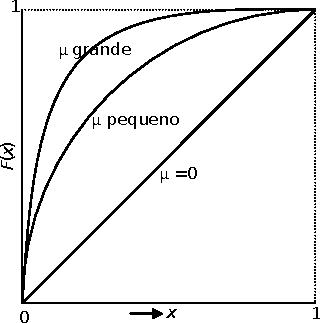
\includegraphics[width=0.4\textwidth]{images/mulaw.pdf}
  \caption{Curva de compressores segundo a lei $\mu$ \citep{tokunbo}.}
  \label{fig:mulaw}
  \end{figure}
  
  A lei $\mu$ é utilizada no padrão ITU G.711 PCM através de uma aproximação discreta usando $\mu=255$.
\end{frame}

\begin{frame}[allowframebreaks]
  \frametitle{lei A}

  \begin{figure}[h!]
  \centering
  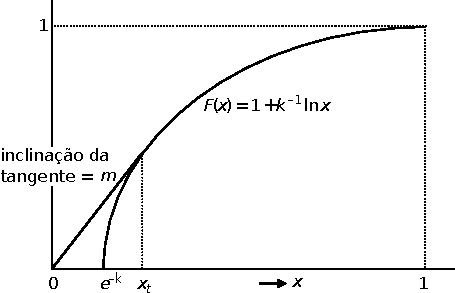
\includegraphics[width=0.6\textwidth]{images/Alaw.pdf}
  \caption{Curva de compressores segundo a lei A \citep{tokunbo}.}
  \label{fig:Alaw}
  \end{figure}

  \begin{equation}
  k = 1 + \ln A .
  \end{equation}

  \begin{equation}
  F(x) = \begin{cases}
  \frac{Ax}{1+\ln A} , \quad 0 \leq x \leq 1/A , \\
  \frac{1+\ln Ax}{1+\ln A}, \quad 1/A \leq x \leq 1 .
  \end{cases}
  \end{equation}

  \bibentry{tokunbo}
  %\printbibliography[keyword={tokunbo},title={Mais informações:}]
\end{frame}


\subsection{Quantização Vetorial}

\begin{frame}[allowframebreaks]
  \frametitle{Quantização Vetorial}
  Utilizamos a quantização vetorial em casos em que o sinal de entrada já é um sinal digital
  e queremos obter uma representação comprimida da informação origial (em geral, representando
  os dados originais através de um \textit{codebook}).

  \vspace{1cm}
  Considere uma variável aleatória $X$ que assumule valores $x \in \mathcal{X} \subseteq \mathit{R}$,
  e $\mathcal{X}^n \subseteq \mathit{R}^n$ o conjunto de vetores $\mathbf{x} = (x_1, x_2, \ldots, x_n) \in \mathit{R}^n$.

  \framebreak

  Uma quantização vetorial é um mapeamento $Q$  de vetores de entrada $\mathbf{x} = (x_1, x_2, \ldots, x_n )$,
  onde $\mathbf{x} \in \mathcal{X}^n$, nos valores $\mathbf{y} = (y_1 , y_2 , \ldots , y_n ) \in \mathcal{X}^n$
  mais próximos (com relação a alguma medida de distorção), onde $\mathbf{y} \in \mathcal{Y} \subseteq \mathcal{X}^n$,
  sendo $\mathcal{Y} = \{y_1 , y_2 , \ldots, y_M\}$, um subconjunto constituído por $M$ elementos em $\mathcal{X}^n$.
  O parâmetro $n$ indica a dimensionalidade dos dados e do quantizador. O conujunto de aproximação $\mathcal{Y}$ 
  é chamado de \textit{codebook}.

  \vspace{3em}
  Para se projetar um quantizador, devemos dividir o domínio $\mathcal{X}^n$ em $M$ áreas ou células $S_i$,
  $i = 1, 2, \ldots, M$, de forma que $\bigcup_i S_i = \mathcal{X}^n$, $S_i \cap S_j = \emptyset$, $i \neq j$,
  e $y_i \in S_i$.
\end{frame}


\begin{frame}[allowframebreaks]
  \frametitle{Erro de quantização médio}
  O erro de quantização esperado de um quantizador é dado por
  \begin{equation}
  D_n(Q) = E \{ d(\mathbf{x},Q(\mathbf{x})) \}
  \end{equation}

  Utilizando a distância Euclideana normalizada como métrica
  \begin{eqnarray}
  d(\mathbf{x},\mathbf{y}) &=& \frac{1}{n} d^2_E(\mathbf{x},\mathbf{y}) \nonumber \\
                           &=& \frac{1}{n} (\mathbf{x} - \mathbf{y}) (\mathbf{x} - \mathbf{y})^T \nonumber \\
                           &=& \frac{1}{n} \sum_{i=1}^n (x_i - y_i)^2 = \frac{1}{n} \Vert \mathbf{x} - \mathbf{y} \Vert^2
  \end{eqnarray}
  teremos
  \vspace{-1ex}
  \begin{equation}
  D_n (Q) = \frac{1}{n} E \{ \Vert \mathbf{x} - Q(\mathbf{x}) \Vert^2 \} = \frac{1}{n} \sum_{i=1}^M  E \{ \Vert \mathbf{x} - \mathbf{y_i} \Vert^2 \} .
  \label{eq:avg_quant_error}
  \end{equation}
 
  \framebreak
  Considere que a pdf n-dimensional dos dados, $f(\mathbf{x})$, sobre o conjunto $\mathcal{X}^n$ seja conhecida, 
  então a Equação \ref{eq:avg_quant_error} assume a forma 
  \begin{equation}
  D_n (Q) = \frac{1}{n} \sum_{i=1}^M \int_{S_i} f(\mathbf{x}) \Vert \mathbf{x} - \mathbf{y_i} \Vert^2 \mathrm{d}\mathbf{x} ,
  \end{equation}
  e a probabilidade do vetor de representação $\mathbf{y_i}$ é dada por
  \begin{equation}
  P(\mathbf{y_i}) = \int_{S_i} f(\mathbf{x}) \mathrm{d}\mathbf{x} .
  \end{equation}
\end{frame} 


\begin{frame}%[allowframebreaks]
  \frametitle{Taxa de quantização}
  A taxa de quantização $R$ é o número de bits necessários para representar o vetor $\mathbf{x}$
  (utilizando vetores de \textit{codebook} de tamanho $M$) por dimensão, $n$. Para um quantizador com taxa fixa
  (em que cada símbolo é codificado por palavras de mesmo tamanho em um dado \textit{codebook}), 
  a taxa é dada por
  \begin{equation}
  R = \frac{\log_2 M}{n} \textmd{ bits/amostra}.
  \end{equation}

  Para um quantizador de taxa variável, a taxa estará limitada pela entropia, ou seja,
  \begin{equation}
  R \geq - \frac{1}{n} \sum_{i=1}^M P(\mathbf{y_i}) \log_2 P(\mathbf{y_i}) \textmd{ bits/amostra}.
  \end{equation}
\end{frame}

\begin{frame}[allowframebreaks]
  \frametitle{Quantização vetorial}
  As células criadas por um quantizador vetorial em $n$-dimensões são regiões de Voronoi.

  O caso especial em que o \textit{codebook} gera uma estrutura regular é chamado 
  de quantizador vetorial em treliça (\textit{lattice vector quantizers}).

  \begin{figure}[h!]
  \centering
  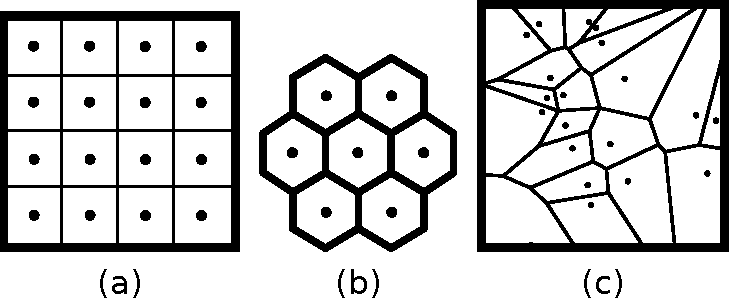
\includegraphics[width=0.6\textwidth]{images/lattice.pdf}
  \caption{Diagramas de Voronoi. Estruturas em treliça em (a) e (b).}
  \label{fig:lattice}
  \end{figure} 
\end{frame}

\begin{frame}%[allowframebreaks]
  \frametitle{Exemplo Quantização - GNU Octave}
  \centering
  
\includegraphics[width=0.4\textwidth]{images/qrcode-jupyter-quantizacao.pdf}

  \url{https://nbviewer.jupyter.org/github/leolca/notebooks/blob/master/aev/quantization.ipynb}
\end{frame} 


\begin{frame}%[allowframebreaks]
  \frametitle{Exemplos de utilização}
  A quantização vetorial é utilizada em
  \begin{itemize}
  \item Video codecs: Cinepak, Sorenson codec, Indeo, VQA (utilizada em jogos)
  \item Audio codecs: CELP, G.729, TwinVQ, Ogg Vorbis, AMR-WB+, DTS
  \end{itemize}
\end{frame}



\subsection{Dithering}

\begin{frame}%[allowframebreaks]
  \frametitle{Quantização vetorial de cores e dithering}

  \bibentry{araujo2018}

  {
  \raggedleft
  
\includegraphics[width=0.15\textwidth]{images/qrcode-artigo-dithering.pdf}
  \url{https://biblioteca.sbrt.org.br/articles/807}
  }
  
  Alguns tópicos abordados no texto:
  \begin{itemize}
  \item quantização vetorial;
  \item espaços de cores;
  \item difusão de erro (\textit{dithering});
  \item dissimilaridade entre imagens.
  \end{itemize}
 
\end{frame}

\begin{frame}%[allowframebreaks]
  \frametitle{Dithering}

  \centering
  
\includegraphics[width=0.3\textwidth]{images/qrcode-jupyter-dithering.pdf}
  \url{https://nbviewer.jupyter.org/github/leolca/notebooks/blob/master/aev/dithering.ipynb}

\end{frame}


\subsection{Processamento digital de sinais analógicos}

\begin{frame}%[allowframebreaks]
  \frametitle{Processamento digital de sinais analógicos}
  \begin{figure}[h!]
  \centering
  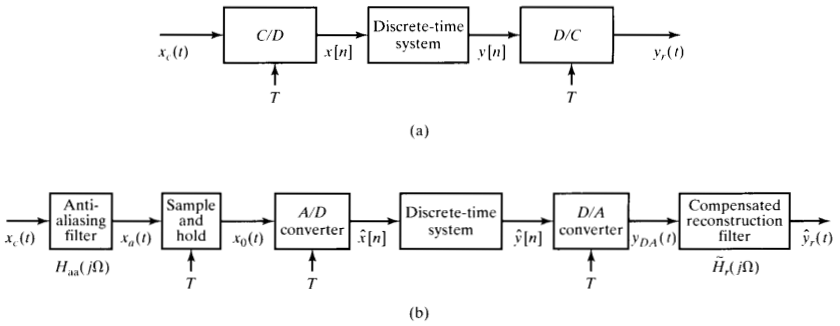
\includegraphics[width=0.9\textwidth]{images/oppenheim_fig441.png}
  \caption{Processamento digital de sinais analógicos \citep{oppenheim2009}.}
  \label{fig:oppenheim_fig441}
  \end{figure}
  \bibentry{oppenheim2009}
\end{frame}
\note{
   Na prática temos que, 
   \begin{itemize}
   \item os sinais contínuos não são estritamente limitados em frequência;
   \item filtros ideais não são realizáveis;
   \item os conversores ideais C/D e D/C são aproximações de conversores A/D (analógico-digital)
        e D/A (digital-analógico).
   \end{itemize}
}
\note{
Devemos utilizar um filtro \textit{anti-aliasing}.

\begin{itemize}
\item usualmente é desejável utilizar uma taxa de amostragem baixa;
\item o próprio sinal e/ou ruído podem aparecer falseados como informação de baixa frequência;
\end{itemize}
}


\begin{frame}%[allowframebreaks]
  \frametitle{Filtro \textit{antialiasing} ideal}
  Resposta em frequência de um filtro \textit{antialiasing} ideal:
  \begin{equation}
  H_{\textmd{aa}} ( j \Omega ) = \begin{cases}1 \quad &, \vert \Omega \vert < \Omega_c < \pi/T ,\\ 
                                   0 &, \vert \Omega \vert > \Omega_c \textmd{.} 
			\end{cases}
  \end{equation}
\end{frame}


\begin{frame}[allowframebreaks]
  \frametitle{Processamento digital de sinais analógicos}

  \begin{figure}[h!]
  \centering
  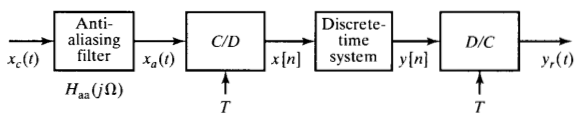
\includegraphics[width=0.8\textwidth]{images/oppenheim_fig442.png}
  \caption{Processamento digital de sinais analógicos \citep{oppenheim2009}.}
  \label{fig:oppenheim_fig442}
  \end{figure}

  \bibentry{oppenheim2009}

  Considerando a entrada $x_a(t)$ e a saída $y_r(t)$, o sistema todo (compreendido entre entrada e saída) 
  pode ser visto como um sistema linear invariante no tempo com resposta $H (e^{j \Omega T})$.

  Assim, a resposta total do sistema será
  \begin{equation}
  H_{\text{eff}} (j \Omega) \approx H_{aa} (j \Omega) H (e^{j \Omega T}) \textmd{,}
  \end{equation}
  ou seja,
  \begin{equation}
    H_{\text{eff}} (j \Omega) \approx \begin{cases} H(e^{j\Omega T}) \quad &, \vert \Omega \vert < \Omega_c,\\ 
                                   0 &, \vert \Omega \vert > \Omega_c \textmd{.} \end{cases}
  \end{equation}
  Na prática, teremos a aproximação acima pois 
  a resposta em frequência de $H_{\text{aa}} (j \Omega)$ não é idealmente limitada em frequência,
  mas podemos fazer $H_{\text{aa}} (j \Omega)$ pequeno para $\vert \Omega \vert > \pi / T$, minimizando assim 
  o \textit{aliasing}.
\end{frame} 
\note{
  Filtros abruptos são de difícil implementação e alto custo. Além disso, geralmente possuem resposta
  em fase altamente não-linear.
  Para que o sistema opere com
  diferentes taxas de amostragem, devemos ter filtros ajustáveis.
} 

\begin{frame}[allowframebreaks]
  \frametitle{Utilizando uma conversão A/D com sobre-amostragem para simplificar o filtro analógico \textit{antialiasing}}

  \begin{figure}[h!]
  \centering
  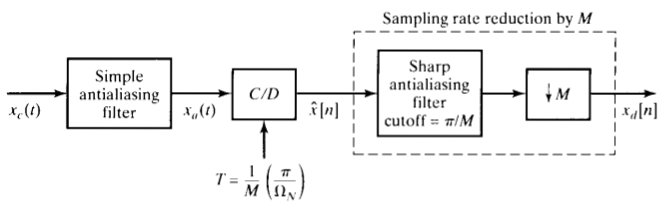
\includegraphics[width=0.6\textwidth]{images/oppenheim_fig443.png}
  \caption{Utilizando uma conversão A/D com sobre-amostragem para simplificar o filtro analógico \textit{antialiasing} \citep{oppenheim2009}.}
  \label{fig:oppenheim_fig443}
  \end{figure}
  \bibentry{oppenheim2009}

  \begin{description}
  \item[$\Omega_N$]: frequência mais alta que desejamos manter
  \item[$M$]: fator de sobre-amostragem
  \end{description}

\end{frame}


\begin{frame}[allowframebreaks]
  \frametitle{Sobre-amostragem e decimação}

  \begin{figure}[h!]
  \centering
  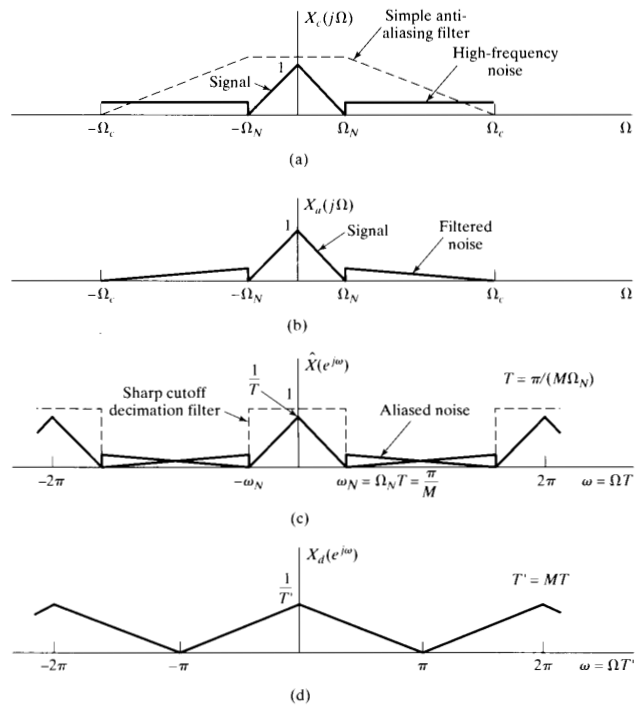
\includegraphics[width=0.35\textwidth]{images/oppenheim_fig444.png}
  \caption{Exemplo \citep{oppenheim2009}}
  \label{fig:oppenheim_fig444}
  \end{figure}
  %{\small \bibentry{oppenheim2009}}

  \begin{figure}[h!]
  \centering
  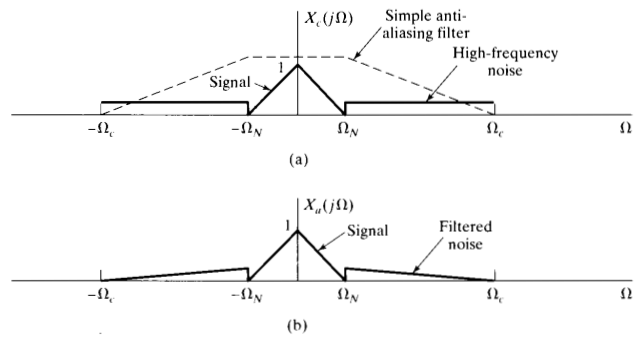
\includegraphics[width=0.8\textwidth]{images/oppenheim_fig444ab.png}
  %\caption{}
  \label{fig:oppenheim_fig444ab}
  \end{figure}

  \begin{figure}[h!]
  \centering
  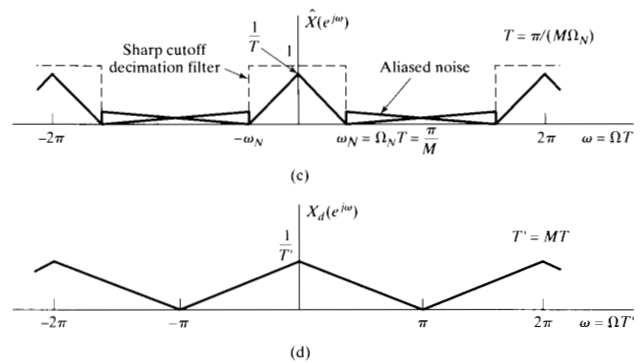
\includegraphics[width=0.8\textwidth]{images/oppenheim_fig444cd.png}
  %\caption{}
  \label{fig:oppenheim_fig444cd}
  \end{figure}

\end{frame}


\begin{frame}%[allowframebreaks]
  \frametitle{Configuração física para conversão analógico-digital}

  \begin{figure}[h!]
  \centering
  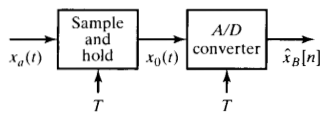
\includegraphics[width=0.6\textwidth]{images/oppenheim_fig445.png}
  \caption{Configuração física para conversão analógico-digital \citep{oppenheim2009}.}
  \label{fig:oppenheim_fig445}
  \end{figure}

  \begin{description}
  \item[$x_a(t)$]: sinal analógico
  \item[{$\hat{x}_{B}[n]$}]: sinal digital (amostrado e quantizado)
  \item[$T$]: período de amostragem
  \end{description}

\end{frame}


\begin{frame}[allowframebreaks]
  \frametitle{Representação de um \textit{sample-and-hold} ideal}

  \hvFloat[floatPos=htb,capPos=right,capVPos=bottom,objectPos=c]{figure}{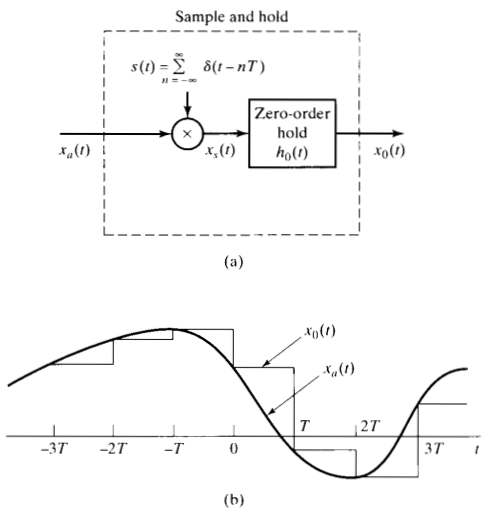
\includegraphics[width=0.45\textwidth]{images/oppenheim_fig446.png}}
  {Sample-and-hold \citep{oppenheim2009}.}{fig:oppenheim_fig446}

  A saída de um \textit{sample-and-hold} ideal é dada por
  \begin{equation}
  x_0(t) = \sum_{n=-\infty}^{\infty} x[n] h_0 (t -nT)
  \label{eq:x0t}
  \end{equation}
  onde $x[n] = x_a(nT)$ são as amostras ideais (não quantizadas) de $x_a(t)$ e 
  $h_0(t)$ é a resposta ao impulso do \textit{hold} de ordem zero, i.e.,
  %where $x[n] = x_a(nT)$ are the ideal samples of $x_a(t)$ and $h_0(t)$ is the impulse response of the zero-order-hold system, i.e.,
  \begin{equation}
  h_0(t) = \begin{cases} 1  \quad &,  0 < t < T ,\\ 
                         0 &, \mbox{caso contrário.}\end{cases} 
  \end{equation}
  A Equação \ref{eq:x0t} é equivalente a
  %The Equation \ref{eq:x0t} has the equivalent form
  \begin{equation}
  x_0(t) = h_0(t) \ast \sum_{n=-\infty}^{\infty} x_a(nT) \delta(t-nT) \textmd{ . }
  \end{equation}
\end{frame}
\note{
O circuito de uma \textit{sample-and-hold} é projetado para amostrar $x_a(t)$ `instantaneamente'
e `manter' o valor da amostra constante até que a próxima amostra seja tomada. Isto é necessário
para fornecer uma tensão de entrada constante no conversor A/D.
}

\begin{frame}%[allowframebreaks]
  \frametitle{Equivalência Conceitual}
  O sistema composto pelo \textit{sample-and-hold} seguido por um conversor A/D
  \begin{figure}[h!]
  \centering
  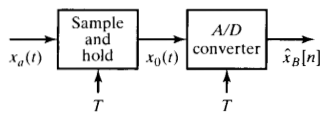
\includegraphics[width=0.4\textwidth]{images/oppenheim_fig445.png}
  %\caption{}
  \label{fig:oppenheim_fig445_2}
  \end{figure}
  é equivalente ao seguinte sistema, composto por um conversor C/D ideal seguido por um quantizador
  \begin{figure}[h!]
  \centering
  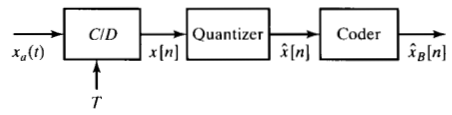
\includegraphics[width=0.6\textwidth]{images/oppenheim_fig447.png}
  \caption{Sistema equivalente \citep{oppenheim2009}.}
  \label{fig:oppenheim_fig447}
  \end{figure}
\end{frame}

\begin{frame}[allowframebreaks]
  \frametitle{Quantizador Uniforme}
  Um quantizador é um sistema não-linear cuja operação é definida por uma função $Q(\cdot)$,
  \begin{equation}
  \hat{x}[n] = Q(x[n]) .
  \end{equation}

  \framebreak

  \hvFloat[floatPos=htb,capPos=right,capVPos=bottom,objectPos=c]{figure}{\includegraphics[width=0.7\textwidth]{images/oppenheim_fig448.png}}
  {Quantizador uniforme de 3 bits \citep{oppenheim2009}.}{fig:oppenheim_fig448}


%  \begin{figure}[h!]
%  \centering
%  \includegraphics[width=0.7\textwidth]{/home/leoca/ee/ufsj/2014_01/audiovideo/aula/images/oppenheim_fig448.png}
%  \caption{Quantizador uniforme de 3 bits \citep{oppenheim2009}.}
%  \label{fig:oppenheim_fig448}
%  \end{figure}

  \framebreak

  O bit mais à esquerda, o bit mais significativo, é considerado o bit de sinal. 
  Os demais bits representam na forma binária uma fração (ou inteiro).
  \begin{figure}[h!]
  \centering
  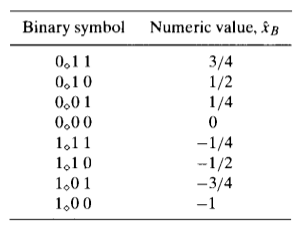
\includegraphics[width=0.4\textwidth]{images/oppenheim_tab_bincode.png}
  \caption{Código binário: complemento de dois \citep{oppenheim2009}.}
  \label{fig:oppenheim_tab_bincode}
  \end{figure}
  De forma geral, temos $(B+1)$-bits, complemento de 2 de uma fração binária na forma 
  $a_0 . a_1 a_2 \ldots a_B$, cujo valor é
  \begin{equation}
  -a_0 2^0 + a_1 2^{-1} + a_2 2^{-2} + \cdots + a_B 2^{-B} \textmd{ .}
  \end{equation}

  \framebreak

  \begin{description}
  \item[$X_m$]: estensão do sinal na entrada do conversor A/D
  \item[$\Delta$]: tamanho do passo do quantizador
  \item[$B+1$]: número de bits do quantizador
  \end{description}
 
  \begin{equation}
  \label{eq-Xm-B}
  \Delta = \frac{2 X_m}{2^{B+1}} = \frac{X_m}{2^B} \textmd{ .}
  \end{equation}

  A relação entre as palavras do quantizador e as amostras quantizadas é dada por
  \begin{equation}
  \hat{x}[n] = X_m \hat{x}_B [n] \textmd{ ,}
  \end{equation}
  pois assumimos que $\hat{x}_B [n]$ é um número binário $-1 \leq \hat{x}_B [n] < 1$ (complemento de dois).

  Para simplificar, podemos assumir que o sinal de entrada é normalizado.

\end{frame}

\begin{frame}[allowframebreaks]
  \frametitle{Erro de quantização} 

  O erro de quantização é definido por
  \begin{equation}
  e[n] = \hat{x} [n] - x[n] \textmd{ .}
  \end{equation}

  O erro de quantização satisfaz
  \begin{equation}
  \ \Delta/2 < e[n] \leq \Delta/2
  \end{equation}
  sempre que
  \begin{equation}
  (- X_m - \Delta/2) < x[n] \leq (X_m - \Delta/2) \textmd{ .}
  \end{equation}
  Se $x[n]$ estiver fora desta faixa, o erro de quantização será maior do que $\Delta/2$, e as amostras
  serão `grampeadas'.
\end{frame}

\begin{frame}[allowframebreaks]
  \frametitle{Modelo aditivo do erro de quantização}
  \begin{figure}[h!]
  \centering
  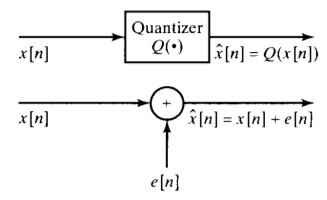
\includegraphics[width=0.4\textwidth]{images/oppenheim_fig450.png}
  \caption{Modelo aditivo do erro de quantização \citep{oppenheim2009}.}
  \label{fig:oppenheim_fig450}
  \end{figure}

  \vspace{-2ex}
  \begin{small}
  A representação estatística do erro de quantização é baseada nas seguintes suposições:
  \begin{itemize}
  \item $e[n]$ é um processo estocástico estacionário;
  \item $e[n]$ é descorrelacionada com $x[n]$;
  \item o erro é um ruído branco, suas amostras são descorrelacionadas
  \item a pdf do erro é uniforme 
  \end{itemize}
  \end{small}
  
  \framebreak

  Para $\Delta$ pequeno, podemos assumir que $e[n]$ é um ruído branco uniforme em $[-\Delta/2, \Delta/2]$.

  \begin{figure}[h!]
  \centering
  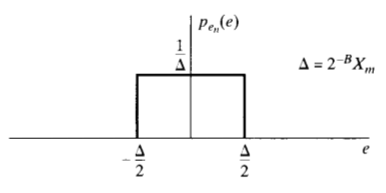
\includegraphics[width=0.55\textwidth]{images/oppenheim_fig452.png}
  \caption{Modelo do ruído \citep{oppenheim2009}.}
  \label{fig:oppenheim_fig452}
  \end{figure}

  \begin{description}
  \item[média]: $\mu_e = 0$;
  \item[variância]: $\sigma_e^2 = \Delta^2/12$.
  \end{description}

  \begin{equation}
  \sigma_e^2 = \int_{-\Delta/2}^{\Delta/2} e^2 \frac{1}{\Delta} de = \frac{\Delta^2}{12} \textmd{ .}
  \end{equation}

  Para um quantizador de $(B+1)$ bits e fundo de escala $X_m$, a variância do ruído (ou potência)
  será dada por
  \begin{equation}
  \sigma_e^2 = \frac{2^{-2B}X_m^2}{12} \textmd{ ,}
  \end{equation}
  onde $\Delta = X_m/2^B$.


  \framebreak

  A relação sinal-ruído de quantização para um quantizador com $(B+1)$ bits é
  \begin{eqnarray}
  \textmd{SQNR} &=& 10 \log_{10} \left( \frac{\sigma_x^2}{\sigma_e^2} \right) = 10 \log_{10} \left( \frac{12 \cdot 2^{2B} \sigma_x^2}{X_m^2} \right) \nonumber \\
      &=& 6.02 B + 10.8 - 20 \log_{10} \left( \frac{X_m}{\sigma_x} \right) \textmd{ .}
  \end{eqnarray}
  Aproximadamente 6dB para cada bit.

\end{frame} 


\subsection{Conversão discreto-contínuo}
\begin{frame}[allowframebreaks]
  \frametitle{Conversão discreto-contínuo}
  \begin{figure}[h!]
  \centering
  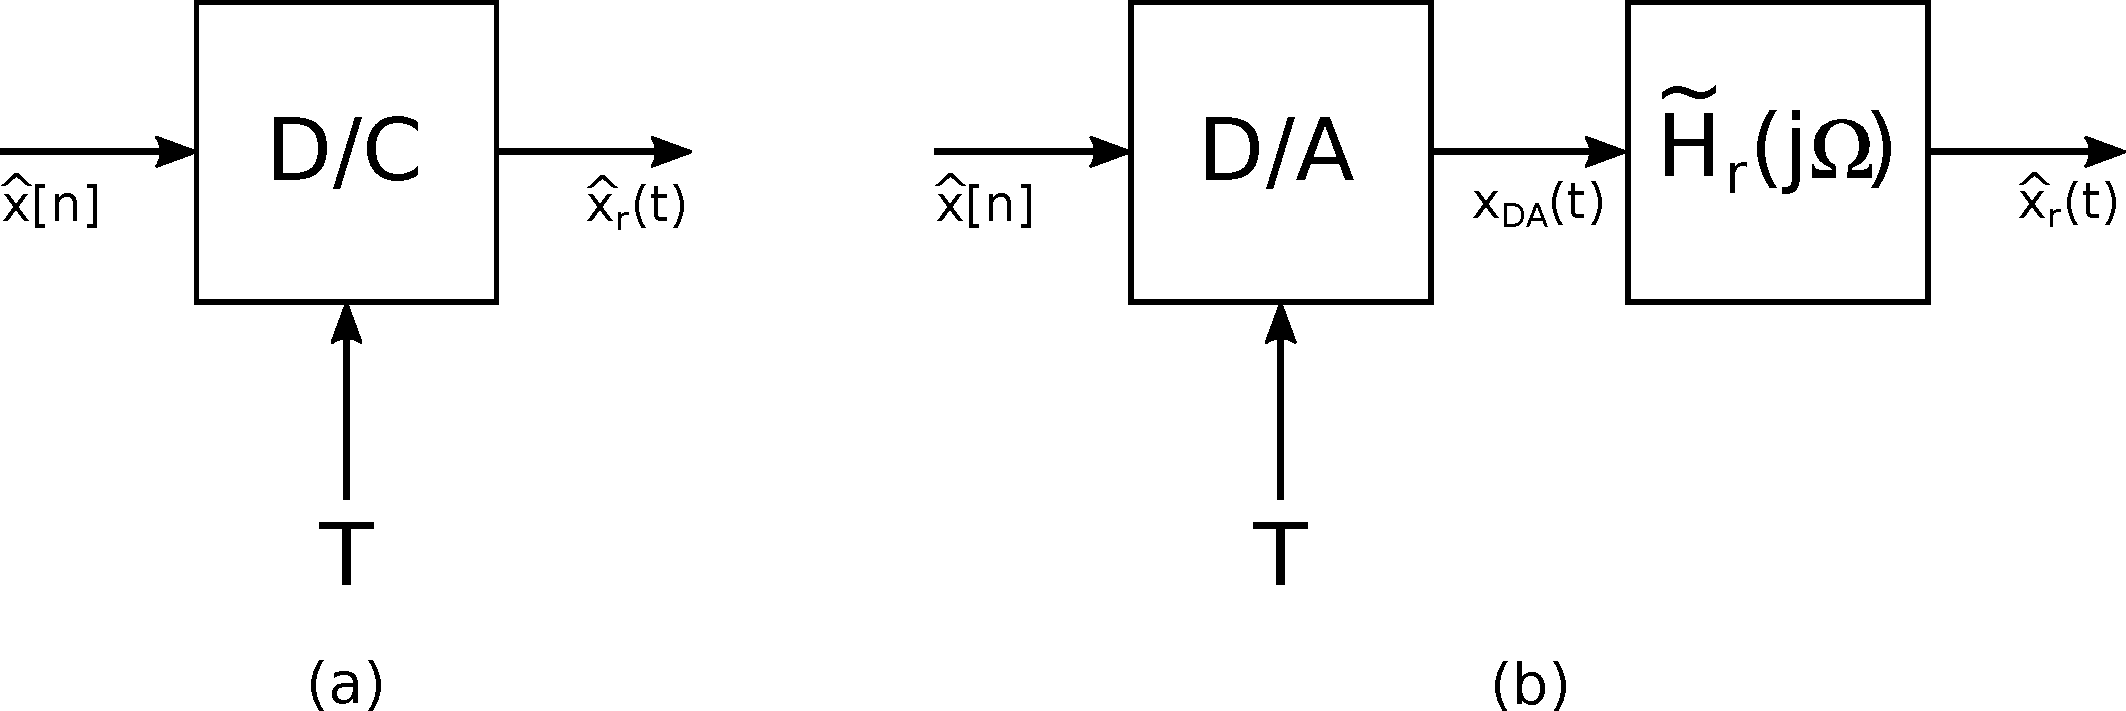
\includegraphics[width=0.8\textwidth]{images/da-conversion.pdf}
  \caption{Conversão discreto para contínuo.}
  \label{fig:da-conversion}
  \end{figure}

  \framebreak

  A reconstrução é representada por
  \begin{equation}
  X_r (j\Omega) = X(e^{j\Omega T}) H_r(j\Omega)
  \end{equation}
  onde $X(e^{j\Omega})$ é a transformada discreta de Fourier de $x[n]$ e $X_r(j\Omega)$
  é a transformada de Fourier do sinal reconstruído. O filtro de reconstrução ideal é dado por
  \begin{equation}
  H_r(j\Omega) = \begin{cases} T  \quad &, |\Omega|  < \pi/T ,\\ 0 &, |\Omega| > \pi/T \textmd{ .}\end{cases}
  \end{equation}
  A relação entre $x_r(t)$ e $x[n]$ será dada por
  \begin{equation}
  x_r (t) = \sum_{n=-\infty}^{\infty} x[n] \frac{\sin [\pi (t-nT)/T]}{\pi(t-nT)/T} \textmd{ .}
  \end{equation}

  \framebreak

  \begin{figure}[h!]
  \centering
  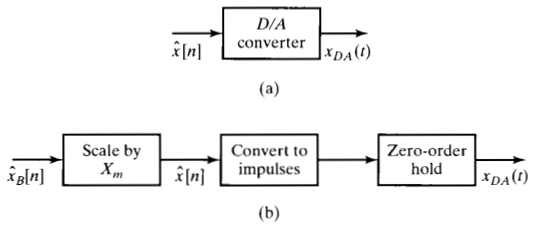
\includegraphics[width=0.5\textwidth]{images/oppenheim_fig453.png}
  \caption{Modelo do conversor D/A \citep{oppenheim2009}.}
  \label{fig:oppenheim_fig453}
  \end{figure}

  \begin{eqnarray}
  x_{\text{DA}}(t) &=& \sum_{n=-\infty}^{\infty} X_m \hat{x}_B[n] h_0(t-nT) \nonumber \\
            &=& \sum_{n=-\infty}^{\infty} \hat{x}[n] h_0(t-nT) \textmd{ .}
  \end{eqnarray}

  \framebreak

  Utilizando o modelo aditivo do ruído de quantização (ver \Cref{fig:oppenheim_fig450}),
  podemos considerar $x_{\text{DA}}(t)$ como composta em duas partes, uma devida ao sinal
  e outra devida ao ruído de quantização. Assim podemos analisar os efeitos da quantização.

  \begin{equation}
   x_{\text{DA}}(t) = \sum_{n=-\infty}^{\infty} x[n]h_0(t-nT) + \sum_{n=-\infty}^{\infty} e[n] h_0(t-nT) \textmd{ .}
  \end{equation}

  Definimos
  \begin{equation}
  \label{eq-x0t}
  x_0(t) = \sum_{n=-\infty}^{\infty} x[n]h_0(t-nT) \textmd{ , e}
  \end{equation}
  \begin{equation}
  \label{eq-e0t}
  e_0(t) = \sum_{n=-\infty}^{\infty} e[n] h_0(t-nT) \textmd{ ,}
  \end{equation}
  de forma que
  \begin{equation}
  x_{\text{DA}}(t) = x_0(t) + e_0(t) \textmd{ .}
  \end{equation}

  A transformada de Fourier da Equação \ref{eq-x0t} é
  \begin{eqnarray}
  X_0(j\Omega) &=& \sum_{n=-\infty}^{\infty} x[n] H_0(j\Omega) e^{-j \Omega nT} \nonumber \\
               &=& \left( \sum_{n=-\infty}^{\infty} x[n] e^{-j \Omega nT} \right) H_0(j\Omega) \nonumber \\
               &=& X(e^{j\Omega T}) H_0(j\Omega) \textmd{ .}
  \end{eqnarray}
  Como
  \vspace{-0.2cm}
  \begin{equation}
  X(e^{j\Omega T}) = \frac{1}{T} \sum_{k=-\infty}^{\infty} X_a \left( j \left( \Omega - \frac{2\pi k}{T} \right) \right) .
  \end{equation}
  segue que
  \vspace{-0.2cm}
  \begin{equation}
  \label{eq-X0jomega}
  X_0(j\Omega) = \left[  \frac{1}{T} \sum_{k=-\infty}^{\infty} X_a \left( j \left( \Omega - \frac{2\pi k}{T} \right) \right) \right] H_0(j\Omega) \textmd{ .}
  \end{equation}
\end{frame}

\begin{frame}[allowframebreaks]
  \frametitle{Filtro de Reconstrução}
  Se $X_a(j \Omega)$ é limitado em frequência abaixo de $\pi/T$,
  as cópias deslocadas de $X_a(j \Omega)$ não se sobrepõem na Equação \ref{eq-X0jomega},
  e se definirmos o filtro de reconstrução compensado como
  \begin{equation}
  \tilde{H}_r (j\Omega) = \frac{H_r (j\Omega)}{H_0(j \Omega)},
  \end{equation}
  então, a saída do filtro será $x_a(t)$ se a entrada for $x_0(t)$.
  A resposta em frequência do \textit{hold} de ordem zero é
  \begin{equation}
  H_0 (j\Omega) = \frac{2 \sin(\Omega T/2)}{\Omega} e^{-j\Omega T/2} .
  \end{equation}
  Desta forma, o filtro de reconstrução compensado é dado por
  \begin{equation}
  \tilde{H}_r (j\Omega) = \begin{cases}\frac{\Omega T/2}{\sin(\Omega T/2)} e^{j \Omega T /2} \quad & |\Omega| \leq \pi/T ,\\
                                     0 & |\Omega| > \pi/T .\end{cases}
  \end{equation}

  \begin{figure}[h!]
  \centering
  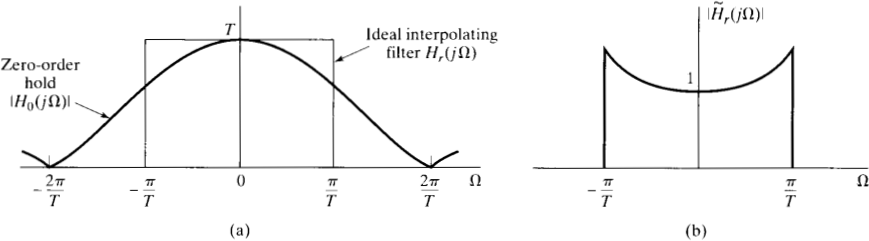
\includegraphics[width=0.8\textwidth]{images/oppenheim_fig454.png}
  \caption{Filtro de reconstrução compensando o efeito do hold \citep{oppenheim2009}.}
  \label{fig:oppenheim_fig454}
  \end{figure}

\end{frame}


\begin{frame}[allowframebreaks]
  \frametitle{Configuração física da conversão digital analógico}
  \begin{figure}[h!]
  \centering
  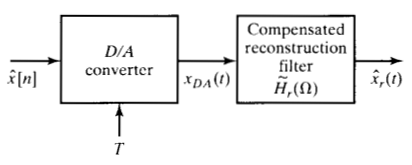
\includegraphics[width=0.5\textwidth]{images/oppenheim_fig455.png}
  \caption{Configuração física para a conversão digital-analógico \citep{oppenheim2009}.}
  \label{fig:oppenheim_fig455}
  \end{figure}

  \framebreak 
  O sinal reconstruído na saída é
  \begin{eqnarray}
  \hat{x}_r (t) &=& \sum_{n=-\infty}^{\infty} \hat{x}[n] \frac{\sin [\pi (t - nT)/T]}{\pi (t - nT)/T} \\
                &=& \sum_{n=-\infty}^{\infty} x[n] \frac{\sin [\pi (t - nT)/T]}{\pi (t - nT)/T} + 
                    \sum_{n=-\infty}^{\infty} e[n] \frac{\sin [\pi (t - nT)/T]}{\pi (t - nT)/T} . \nonumber
  \end{eqnarray}
  Ou seja, a saída é dada por 
  \begin{equation}
  \hat{x}_r (t) = x_a(t) + e_a(t),
  \end{equation}
  onde $e_a(t)$ é o ruído branco limitado em frequência.

\end{frame}


\begin{frame}[allowframebreaks]
  \frametitle{Sistema para processamento digital de sinais analógicos}
  %System for digital processing of analog signals}
  \begin{figure}[h!]
  \centering
  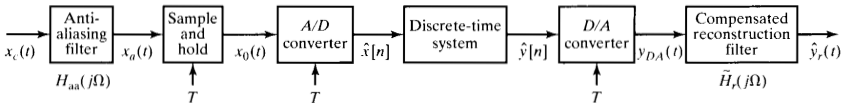
\includegraphics[width=\textwidth]{images/oppenheim_fig441b.png}
  \caption{Sistema para processamento digital de sinais analógicos \citep{oppenheim2009}.}
  \label{fig:oppenheim_fig441b}
  \end{figure}

  \begin{equation}
  \hat{y}_r (t) = y_a (t) + e_a (t)
  \end{equation}
  
  \begin{equation}
  Y_a(j\Omega) = \tilde{H}_r(j\Omega) H_0(j\Omega) H(e^{j\Omega T}) H_{\text{aa}}(j\Omega) X_c(j\Omega) 
  \end{equation}
  onde 
  \begin{itemize}
  \item $H_{\text{aa}}(j\Omega)$ filtro \textit{antialiasing}
  \item $H_0(j\Omega)$ \textit{hold} de ordem zero do conversor D/A 
  \item $\tilde{H}_r(j\Omega)$ filtro passa-baixas de reconstrução 
  \end{itemize}

  
  Assumindo que o ruído de quantização introduzido pelo conversor A/D é branco com
  variância $\sigma_e^2 = \Delta^2/12$, podemos mostrar que o espectro de densidade de potência do ruído na saída é
  \begin{equation}
  P_{e_a} (j\Omega) = \vert \tilde{H}_r(j\Omega) H_0(j\Omega) H(e^{j\Omega T}) \vert^2 \sigma_e^2 .
  \end{equation}
  A resposta em frequência efetiva total de $x_c(t)$ a $y_r(t)$ é
  \begin{equation}
  H_{\text{eff}}(j\Omega) = \tilde{H}_r(j\Omega) H_0(j\Omega) H(e^{j\Omega T}) H_{\text{aa}}(j\Omega) .
  \end{equation}
\end{frame}



%\begin{frame}%[allowframebreaks]
%  \frametitle{}
%\end{frame}

%\begin{frame}%[allowframebreaks]
%  \frametitle{}
%\end{frame}

%\begin{frame}%[allowframebreaks]
%  \frametitle{}
%\end{frame}



% add here: multi rate signal processing
\subsection{Oversampling e Noise-Shaping}


\begin{frame}%[allowframebreaks]
  \frametitle{Oversampling e Noise-Shaping}
  Realizar uma sobre-amostragem (\textit{oversampling}) e, subsequente,
  uma filtragem passa-baixas discreta e uma decimação (\textit{down-sampling})
  permite uma redução no número de bits do quantizador, para uma mesma relação
  sinal-ruído-de-quantização (SQNR\footnote{Signal-to-Quantization-Noise Ratio}). 
  Mantendo número de bits do quantizador, é possível reduzir a SQNR.
\end{frame}

\begin{frame}[allowframebreaks]
  \frametitle{Conversão A/D com sobre-amostragem e quantização direta}
  Considere o sinal de entrada $x_a(t)$:
  \begin{itemize}
  \item média nula
  \item estacionário no sentido amplo 
  \item processo estocástico com densidade espectral de potência $\Phi_{x_a x_a}(j\Omega)$
  \item função de auto-correlação $\phi_{x_a x_a}(\tau)$
  \item limitado em frequência em $\Omega_N$: $\Phi_{x_a x_a}(j\Omega) = 0$, $\Omega \ge \Omega_N$
  \end{itemize}
  Vamos assumir que $2\pi / T = 2 M \Omega_N$. A constante inteira $M$ é o fator de sobre-amostragem.

  \framebreak 

  \begin{figure}[h!]
  \centering
  \includegraphics[width=0.8\textwidth]{images/oppenheim_fig456.png}
  \caption{Conversão A/D com sobre-amostragem \citep{oppenheim2009}.}
  \label{fig:oppenheim_fig456}
  \end{figure}

  \framebreak

  Utilizando o modelo do ruído aditivo.
  \begin{figure}[h!]
  \centering
  \includegraphics[width=\textwidth]{images/oppenheim_fig457.png}
  \caption{Modelo do ruído aditivo na conversão A/D com sobre-amostragem \citep{oppenheim2009}.}
  \label{fig:oppenheim_fig457}
  \end{figure}
  A saída $x_d[n]$ possui duas componentes: $x_{da}[n]$ (devido ao sinal $x_a(t)$) e $x_{de}[n]$ (devido ao ruído $e[n]$).

  Vamos analisar o efeito de cada componente na saída.

  \framebreak 

  Primeiramente vamos considerar o efeito da componente sinal.

  $\phi_{xx}[m]$ e $\Phi(e^{j\omega})$ são autocorrelação e densidade espectral de potência de $x[n]$, respectivamente.
  Por definição
  \begin{equation}
  \phi_{xx}[m] = \varepsilon\{x[n+m] x[n]\} .
  \end{equation}
  Como $x[n]=x_a(nT)$ e $x[n+m]=x_a(nT+mT)$
  \begin{equation}
  \label{eq-exp-xx}
  \varepsilon\{x[n+m] x[n]\} = \varepsilon\{x_a((n+m)T) x_a(nT)\} .
  \end{equation}
  Assim
  \begin{equation}
  \label{eq-phixxm}
  \phi_{xx}[m] = \phi_{x_a x_a} (mT)
  \end{equation}
  i.e., a função de autocorrelação da sequência de amostras é a versão amostrada da
  função de autocorrelação do sinal contínuo correspondente.

  \framebreak

  \Cref{eq-exp-xx,eq-phixxm}, juntamente com a suposição de estacionariedade no sentido amplo, levam a 
  \begin{equation}
  \varepsilon\{x^2[n]\} = \varepsilon\{x_a^2(nT)\} = \varepsilon\{x_a^2(t)\} \quad \textmd{ for all } n \textmd{ or } t.
  \end{equation}
  Como as densidades espectrais de potência são transformadas de Fourier das funções de autocorrelação,
  como consequência da \Cref{eq-phixxm} teremos
  \begin{equation}
  \label{eq-Phixx}
  \Phi_{xx}(e^{j\Omega T}) = \frac{1}{T} \sum_{k=-\infty}^{\infty} \Phi_{x_a x_a} \left( j \left( \Omega - \frac{2\pi k}{T} \right) \right) .
  \end{equation}

  \framebreak

  Assumindo um fator de sobre-amostragem $M$, tal que $2\pi/T = 2M\Omega_N$, substituindo $\Omega = \omega/T$ na \Cref{eq-Phixx}
  \begin{equation}
  \label{eq-Phixxiw}
  \Phi_{xx} (e^{j\omega}) = \begin{cases} \frac{1}{T} \Phi_{x_a x_a} \left( j \frac{\omega}{T} \right)   \quad & , |\omega| < \pi/M,  \\ 
  0 & , \pi/M < \omega \le \pi .\end{cases}
  \end{equation}
  
  \begin{figure}[h!]
  \centering
  \includegraphics[width=0.7\textwidth]{images/oppenheim_fig458.png}
  \caption{Densidade espectral de potência \citep{oppenheim2009}.}
  \label{fig:oppenheim_fig458}
  \end{figure}

  \framebreak

  A potência total do sinal analógico é dada por
  \begin{equation}
  \varepsilon\{x_a^2(t)\} = \frac{1}{2\pi} \int_{-\Omega_N}^{\Omega_N} \Phi_{x_a x_a} (j \Omega) d\Omega .
  \end{equation}
  Pela \Cref{eq-Phixxiw}, a potência total do sinal amostrado é
  \begin{eqnarray}
  \varepsilon\{x^2[n]\} &=& \frac{1}{2\pi} \int_{-\pi}^{\pi} \Phi_{xx}(e^{j\omega}) d\omega \nonumber \\
                        &=& \frac{1}{2\pi} \int_{-\pi/M}^{\pi/M} \frac{1}{T} \Phi_{x_a x_a} \left( j \frac{\omega}{T} \right) d\omega \nonumber \\
                        &=& \frac{1}{2\pi} \int_{-\Omega_N}^{\Omega_N} \Phi_{x_a x_a} (j\Omega) d\Omega = \varepsilon\{x_a^2(t)\} ,
  \end{eqnarray}
  onde utilizamos $\Omega_N T = \pi/M$ e $\Omega = \omega/T$.
  Assim, a potência total do sinal amostrado é igual à potência total do sinal analógico.

  \framebreak
 
  Como $\Phi_{xx}(e^{j\omega})$ é limitado em frequência a $|\omega| < \pi/M$,
  \begin{eqnarray}
  \Phi_{x_{da} x_{da}} (e^{j\omega}) &=& \frac{1}{M} \sum_{k=0}^{M-1} \Phi_{xx} (e^{j(\omega - 2\pi k)/M}) \nonumber \\
                                     &=& \frac{1}{M} \Phi_{xx} (e^{j\omega /M})
  \end{eqnarray}
  A potência total da saída $x_{da}[n]$ é 
  \begin{eqnarray}
  \varepsilon\{x^2_{da}[n]\} &=& \frac{1}{2\pi} \int_{-\pi}^{\pi} \Phi_{x_{da} x_{da}} (e^{j \omega}) d\omega \nonumber = \frac{1}{2\pi} \int_{-\pi}^{\pi} \frac{1}{M} \Phi_{xx} (e^{j\omega/M}) d\omega \nonumber \\
                             &=& \frac{1}{2\pi} \int_{-\pi/M}^{\pi/M} \Phi_{xx} (e^{j\omega}) d\omega = \varepsilon\{x^2 [n]\} .
  \end{eqnarray}
  A potência total da componente de sinal permanece a mesma enquanto atravessa todo o sistema.

  \framebreak

  Considere agora a componente de ruído gerada pela quantização.
  Vamos assumir que $e[n]$ é ruído branco, estacionário no sentido amplo, e
  com variância 
  \begin{equation}
  \label{eq-variance-noise}
  \sigma_e^2 = \frac{\Delta^2}{12} .
  \end{equation}
  Consequentemente, a função de autocorrelação e densidade espectral de potência de $e[n]$
  são dadas, respectivamente, por
  \begin{equation}
  \label{eq-autocorr-noise}
  \phi_{ee} [m] = \sigma_e^2 \delta[m]
  \end{equation}
  e
  \begin{equation}
  \label{eq-power-density-noise}
  \Phi_{ee}(e^{j\omega}) = \sigma_e^2 \quad |\omega| < \pi .
  \end{equation}

  \framebreak

  \begin{figure}[h!]
  \centering
  \includegraphics[width=0.7\textwidth]{images/oppenheim_fig459.png}
  \caption{Densidade espectral de potência do sinal e do ruído \citep{oppenheim2009}.}
  \label{fig:oppenheim_fig459}
  \end{figure}
  À medida que a taxa de sobre amostragem $M$ aumenta, menor será a parte do espectro do ruído
  de quantização que se sobreporá ao espectro do sinal.

  \framebreak

  O filtro passa-baixas ideal remove o ruído de quantização na banda  $\pi/M < |\omega| \le \pi$,
  enquanto deixa a componente de sinal inalterada.
  A potência do ruído na saída do filtro será
  \begin{equation}
  \varepsilon\{ e^2[n] \} = \frac{1}{2\pi} \int_{-\pi/M}^{\pi/M} \sigma_e^2 d\omega = \frac{\sigma_e^2}{M} .
  \end{equation}

  \framebreak

  \begin{figure}[h!]
  \centering
  \includegraphics[width=0.75\textwidth]{images/oppenheim_fig460.png}
  \caption{Densidades espectrais de potência do sinal e ruído, após a decimação \citep{oppenheim2009}.}
  \label{fig:oppenheim_fig460}
  \end{figure}

  \begin{equation}
  \label{eq-qn-power-xde}
  \varepsilon\{ x^2_{de} \} = \frac{1}{2\pi} \int_{-\pi}^{\pi} \frac{\sigma_e^2}{M} d\omega = \frac{\sigma_e^2}{M} = \frac{\Delta^2}{12 M} .
  \end{equation}

  A potência do ruído de quantização $\varepsilon\{ x^2_{de} [n]\}$ reduziu por um fator $M$
  através do filtro e decimação, enquanto a potência do sinal permaneceu inalterada.

  \framebreak

  Utilizando \Cref{eq-qn-power-xde,eq-Xm-B} ($\Delta = X_m/2^B$),
  para uma dada potência de ruído de quantização, existe claramente uma relação
  de compromisso entre o fator de sobre-amostragem $M$ e o passo de quantização $\Delta$.
  \begin{equation}
  \label{eq-pne-MB}
  \varepsilon\{ x^2_{de} [n]\} = \frac{1}{12M} \left( \frac{X_m}{2^B} \right)^2 .
  \end{equation}
  Fixando o quantizador, a potência do ruído pode ser diminuída aumentando o fator de sobre-amostragem $M$.

  \framebreak

  Pela \Cref{eq-pne-MB}, fixando a potência do ruído de quantização $P_{de} = \varepsilon \{ x^2_{de} [n]\}$,
  \begin{equation}
  B = - \frac{1}{2} \log_2 M - \frac{1}{2} \log_2 12 - \frac{1}{2} \log_2 P_{de} + \log_2 X_m .
  \end{equation}
  Para cada vez que dobrarmos o fator de sobre-amostragem $M$, precisaremos de $1/2$ bit a menos
  para obter a mesma relação sinal-ruído-de-quantização 
  (para $M=4$ podemos utilizar um bit a menos e obter a mesma acurácia na representação do sinal).
\end{frame}

\begin{frame}%[allowframebreaks]
  \frametitle{Conversão A/D com \textit{Noise Shaping}}
  O objetivo em da técncia de \textit{noise shaping} é modificar a conversão A/D para que a 
  densidade espectral de potência do ruído de quantização não seja uniforme, de forma que 
  a maior parte de sua potência fique fora da faixa $|\omega| < \pi/M$.
\end{frame}

\begin{frame}[allowframebreaks]
  \frametitle{Conversão A/D com \textit{Noise Shaping}}
  \begin{figure}[h!]
  \centering
  \includegraphics[width=0.7\textwidth]{images/oppenheim_fig461.png}
  \caption{Sistema para conversão A/D com \textit{oversampling} e \textit{Noise Shaping} \citep{oppenheim2009}.}
  \label{fig:oppenheim_fig461}
  \end{figure}
 
  \framebreak

  \begin{figure}[h!]
  \centering
  \includegraphics[width=0.8\textwidth]{images/oppenheim_fig462.png}
  \caption{Modelo de ruído aditivo \citep{oppenheim2009}.}
  \label{fig:oppenheim_fig462}
  \end{figure}

  \framebreak

  \begin{figure}[h!]
  \centering
  \includegraphics[width=0.8\textwidth]{images/oppenheim_fig463.png}
  \caption{Simplificação \citep{oppenheim2009}.}
  \label{fig:oppenheim_fig463}
  \end{figure}

  \framebreak

  Sejam $H_x(z)$ a funcção de transferência de $x[n]$ para $y[n]$ e $H_e(z)$ a função de $e[n]$ para $y[n]$ .

  \begin{equation}
  H_x(z) = 1
  \end{equation}

  \begin{equation}
  H_e(z) = (1 - z^{-1}).
  \end{equation}

  Consequently
  \begin{equation}
  y_x [n] = x[n]
  \end{equation}
 
  \begin{equation}
  \hat{e} [n] = e[n] - e[n-1] 
  \end{equation}

  A saída $y[n]$ poderá ser representada por 
  \begin{equation}
  y [n] = x[n] + \hat{e} [n]
  \end{equation}

  \framebreak

  A densidade espectral de potência do ruído de quantização $\hat{e} [n]$ presente em $y[n]$ é
  \begin{eqnarray}
  \Phi_{\hat{e}\hat{e}} (e^{j\omega}) &=& \sigma_e^2 |H_e (e^{j\omega})|^2 \nonumber \\
                                      &=& \sigma_e^2 [2 \sin(\omega/2) ]^2 .
  \end{eqnarray}

  \begin{figure}[h!]
  \centering
  \includegraphics[width=0.6\textwidth]{images/oppenheim_fig464.png}
  \caption{Densidade espectral de potência do ruído de quantização com \textit{noise shaping} \citep{oppenheim2009}.}
  \label{fig:oppenheim_fig464}
  \end{figure}

  \framebreak

  Densidade espectral de potência após do \textit{downsampling}.
  \begin{figure}[h!]
  \centering
  \includegraphics[width=0.7\textwidth]{images/oppenheim_fig465.png}
  \caption{Densidade espectral de potência final \citep{oppenheim2009}.}
  \label{fig:oppenheim_fig465}
  \end{figure}

  \framebreak

  A potência do sinal $x_{da}[n]$ é
  \begin{equation}
  P_{da} = \varepsilon \{ x^2_{da}[n] \} = \varepsilon \{ x^2[n] \} = \varepsilon \{ x_a^2(t) \} .
  \end{equation}
  A potência do ruído de quantização final na saída é
  \begin{equation}
P_{de} = \frac{1}{2\pi} \int_{-\pi}^{\pi} \Phi_{x_{de} x_{de}} (e^{j\omega}) d\omega = \frac{1}{2\pi} \frac{\Delta^2}{12 M} \int_{-\pi}^{\pi} \left( 2 \sin \left( \frac{\omega}{2M} \right) \right)^2 d\omega
  \end{equation}
  Podemos assumir que $M$ é suficientemente grande e assim
  \begin{equation}
  \sin \left( \frac{\omega}{2M} \right) \approx \frac{\omega}{2M} ,
  \end{equation}
  Assim, poderemos considerar
  \begin{equation} 
  \label{eq-Pde-M}
  P_{de} = \frac{1}{36} \frac{\Delta^2 \pi^2}{M^3} .
  \end{equation}

  \framebreak

  Usando \Cref{eq-Pde-M}, teremos uma relação de compromisso entre o fator de sobre-amostragem $M$
  e o tamanho do passo de quantização $\Delta$.

  \vspace{2ex}
  Para obter uma determinada potência $P_{de}$ devemos ter
  \begin{equation}
  B = - \frac{3}{2} \log_2 M + \log_2 (\pi/6) - \frac{1}{2} \log_2 P_{de} + \log_2 X_m .
  \end{equation}


  \framebreak

  \begin{figure}[h!]
  \centering
  \includegraphics[width=0.5\textwidth]{images/oppenheim_tab41.png}
  \caption{Economia de bits \citep{oppenheim2009}.}
  \label{fig:oppenheim_tab41}
  \end{figure}

  \framebreak

  \begin{figure}[h!]
  \centering
  \includegraphics[width=0.8\textwidth]{images/oppenheim_fig466.png}
  \caption{Estratégia incorporando um segundo estágio \citep{oppenheim2009}.}
  \label{fig:oppenheim_fig466}
  \end{figure}

  \framebreak

  Utilizando um segundo estágio ($p=2$), a função de transferência será da forma
  \begin{equation}
  H_e (z) = (1 - z^{-1})^2 , 
  \end{equation}
  e a densidade espectral de potência na saída em $y[n]$ será
  \begin{equation}
  \Phi_{\hat{e}\hat{e}} (e^{j\omega}) = \sigma_e^2 [2 \sin (\omega /2)]^4 .
  \end{equation}

  \vspace{2ex}
  De forma geral, para $p$ estágios, teremos
  \begin{equation}
  \Phi_{\hat{e}\hat{e}} (e^{j\omega}) = \sigma_e^2 [2 \sin (\omega /2)]^{2p} .
  \end{equation}

  \framebreak

  \begin{figure}[h!]
  \centering
  \includegraphics[width=0.5\textwidth]{images/oppenheim_tab42.png}
  \caption{Redução no número de bits no quantizador para diferentes configurações \citep{oppenheim2009}.}
  \label{fig:oppenheim_tab42}
  \end{figure}

\end{frame}

\begin{frame}[allowframebreaks]
  \frametitle{\textit{Oversampling} e \textit{Noise Shaping} na Conversão D/A}

  A técnica de \textit{Oversampling} e \textit{Noise Shaping} pode ser utilizada na
  conversão D/A quando utiliza-se um conversor D/A mais simples, com menos bits.

  \begin{figure}[h!]
  \centering
  \includegraphics[width=0.8\textwidth]{images/oppenheim_fig467.png}
  \caption{Utilizanção do \textit{oversampling} com um conversor D/A simples \citep{oppenheim2009}.}
  \label{fig:oppenheim_fig467}
  \end{figure}

  \framebreak

  \begin{figure}[h!]
  \centering
  \includegraphics[width=0.5\textwidth]{images/oppenheim_fig468.png}
  \caption{Sistema de \textit{noise shaping} de primeira ordem \citep{oppenheim2009}.}
  \label{fig:oppenheim_fig468}
  \end{figure}

  \framebreak

  \begin{figure}[h!]
  \centering
  \includegraphics[width=0.45\textwidth]{images/oppenheim_fig469.png}
  \caption{Modelo de ruído aditivo para o quantizador \citep{oppenheim2009}.}
  \label{fig:oppenheim_fig469}
  \end{figure}

  \framebreak

  A função de transferência de $\hat{y}[n]$ para $y[n]$ é $H_y(z)=1$ e
  a função $H_e(z)$, de $e[n]$ para $y[n]$, é $H_e(z) = 1 - z^{-1}$.
  
  A densidade espectral de potência, na saída, da componente relativa ao ruído de quantização $\hat{e}[n]$ será
  \begin{equation}
  \Phi_{\hat{e}\hat{e}} (e^{j\omega}) = \sigma_e^2 (2 \sin \omega / 2)^2 ,
  \end{equation}
  onde $\sigma_e^2 = \Delta^2 / 12$.

  \framebreak

  \begin{figure}[h!]
  \centering
  \includegraphics[width=0.3\textwidth]{images/oppenheim_fig470.png}
  \caption{Densidade espectral de potência do sinal e ruído de quantização, na saída \citep{oppenheim2009}.}
  \label{fig:oppenheim_fig470}
  \end{figure}

  \framebreak

  \begin{figure}[h!]
  \centering
  \includegraphics[width=0.65\textwidth]{images/oppenheim_fig470cd.png}
  \caption{Detalhe: densidade espectral de potência do ruído de quantização, na saída \citep{oppenheim2009}.}
  \label{fig:oppenheim_fig470}
  \end{figure}

  \framebreak

  Aplicando a técnica em multi-estágio, podemos obter na saída um espectro da forma
  \begin{equation}
  \Phi_{\hat{e}\hat{e}} (e^{j\omega}) = \sigma_e^{2} (2 \sin \omega /2)^{2p},
  \end{equation}
  empurrando ainda mais o ruído para altas frequências, podendo assim relaxar 
  as condições sobre o filtro de reconstrução.

\end{frame}

%\begin{frame}%[allowframebreaks]
%  \frametitle{}
%\end{frame}

%\begin{frame}%[allowframebreaks]
%  \frametitle{}
%\end{frame}

%\begin{frame}%[allowframebreaks]
%  \frametitle{}
%\end{frame}

%\begin{frame}%[allowframebreaks]
%  \frametitle{}
%\end{frame}



% downsampling and upsampling
\section{Mudança de frequência de amostragem}

\begin{frame}%[allowframebreaks]
  \frametitle{Mudança da Frequência de Amostragem}
  Muitas vezes é necessário mudar a frequência de amostragem de um sinal
  \begin{itemize}
  \item downsample / decimate
  \item upsample / zero pad
  \item reamostragem
  \item fatores inteiros / racionais
  \item interpolação
  \end{itemize}

  Representação de um sinal contínuo através de um sinal discreto (sequencia de amostras).
  \begin{equation}
   x[n] = x_c (nT)
  \end{equation}

  Muitas vezes é necessário alterar a frequência de amostragem de um sinal.
  \begin{equation}
   x'[n] = x_c(nT')
  \end{equation}
  onde $T'\neq T$

  Embora seja sempre possível reconstruir um sinal contínuo limitado em frequência e
  realizar uma nova amostragem deste sinal, queremos um processamento puramente discreto.
\end{frame}


\subsection{Downsampling}
\begin{frame}[allowframebreaks]
  \frametitle{Downsample por um fator inteiro}
  Podemos reduzir a frequência de amostragem de uma sequência `amostrando'-a e assim
  gerando uma nova sequência.

  Reduzir a frequência de amostragem por um fator $M$
  \begin{equation}
   x_d[n] = x[nM] = x_c(nMT)
  \end{equation}

        \begin{figure}[h!]
        \centering
        \includegraphics[width=0.4\textwidth]{images/fig419.pdf}
        \caption{Representação de um compressor ou amostrador discreto. \citep{oppenheim2009}.}
        \label{fig:fig419}
        \end{figure}

  A transformada discreta de Fourier de $x[n] = x_c(nT)$ é
  \begin{equation}
  X(e^{j\omega}) = \frac{1}{T} \sum_{k=-\infty}^{\infty} X_c \left( j \left( \frac{\omega}{T} - \frac{2 \pi k}{T} \right) \right) .
  \end{equation}

  A transformada discreta de Fourier de $x_d[n] = x[nM] = x_c(nT')$, onde $T'=MT$, é
  \begin{align}
   X_d(e^{j\omega}) &= \frac{1}{T'} \sum_{k=-\infty}^{\infty} X_c \left( j \left( \frac{\omega}{T'} - \frac{2 \pi k}{T'} \right) \right) \\
                    &= \frac{1}{MT}  \sum_{k=-\infty}^{\infty} X_c \left( j \left( \frac{\omega}{MT} - \frac{2 \pi k}{MT} \right) \right)
  \end{align}

  \framebreak
  Podemos fazer o índice do somatório da seguinte forma
  \begin{equation}
  r = i + kM
  \end{equation}
  onde $k$ e $i$ são inteiros tais que $-\infty < k < \infty$ e $0 \leq i \leq M-1$.
  Podemos assim reescrever a equação anterior na seguinte forma:
  \begin{align}
  X_d(e^{j\omega}) &= \frac{1}{M} \sum_{i=0}^{M-1} \left[ \frac{1}{T} \sum_{k=-\infty}^{\infty} X_c \left( j \left( \frac{\omega}{MT} - \frac{2 \pi k}{T} - \frac{2\pi i}{MT} \right) \right)  \right] \\
                   &= \frac{1}{M} \sum_{i=0}^{M-1} X\left( e^{j(\omega - 2\pi i)/M} \right) .
  \end{align}
  Teremos $M$ cópias de $X(e^{j\omega})$ dilatadas por um fator $M$ e transladadas por $2\pi i/M$.


  Não haverá \textit{aliasing} se $X(e^{j\omega})$ for limitado em frequência
  \begin{equation}
  X(e^{j\omega}) = 0 , \quad \omega_N \leq \vert \omega \vert \leq \pi,
  \end{equation}
  e $2\pi/M \geq 2 \omega_N$.

        \begin{figure}[h!]
        \centering
        \includegraphics[width=0.75\textwidth]{images/fig421ab.pdf}
        %\caption{Transformada de Fourier de um sinal limitado em frequência. \cite{oppenheim}).}
        \label{fig:fig421ab}
        \end{figure}

        \begin{figure}[h!]
        \centering
        \includegraphics[width=0.75\textwidth]{images/fig421cd.pdf}
        %\caption{Transformada de Fourier de um sinal limitado em frequência. \cite{oppenheim}).}
        \label{fig:fig421cd}
        \end{figure}

        \begin{figure}[h!]
        \centering
        \includegraphics[width=0.75\textwidth]{images/fig421ef.pdf}
        %\caption{Transformada de Fourier de um sinal limitado em frequência. \cite{oppenheim}).}
        \label{fig:fig421ef}
        \end{figure}


  \framebreak
  De forma geral, para evitar \textit{aliasing} ao realizar um \textit{downsample} por um fator $M$
  é necessário que
  \begin{equation}
  \omega_N M \leq \pi \quad \quad \textmd{ ou } \quad \quad \omega_N \leq \pi/M.
  \end{equation}

        \begin{figure}[h!]
        \centering
        \includegraphics[width=0.65\textwidth]{images/fig422.pdf}
        \caption{Sistema geral para redução da frequência de amostragem por um fator $M$. \citep{oppenheim2009}.}
        \label{fig:fig422}
        \end{figure}

\end{frame}


\subsection{Upsampling}
\begin{frame}[allowframebreaks]
  \frametitle{upsample por um fator inteiro}

  Considere o sinal $x[n]$ o qual queremos aumentar a frequência de amostragem por um fator $L$.

  Vamos considerar o sinal contínuo subjacente $x_c(t)$. O objetivo é obter as amostras
  \begin{equation}
   x_i[n] = x_c(nT')
  \end{equation}
  onde $T'=T/L$, a partir das amostras
  \begin{equation}
   x[n] = x_c(nT .)
  \end{equation}
  Das equações acima, segue que
  \begin{equation}
   x_i[n] = x[n/L] = x_c(nT/L), \quad 0, \pm L, \pm 2 L, \ldots
  \end{equation}

  \framebreak
  Sistema para aumentar a frequência de amostragem por um fator $L$.
        \begin{figure}[h!]
        \centering
        \includegraphics[width=0.65\textwidth]{images/fig423.pdf}
        \caption{Sistema geral para aumentar a frequência de amostragem por um fator $L$. \citep{oppenheim2009}.}
        \label{fig:fig423}
        \end{figure}

  O sistema da esquerda é chamado expansor. Sua saída será
  \begin{equation}
   x_e[n] = \begin{cases} 
      x[n/L] , \quad n = 0, \pm L, \pm 2L, \ldots \\
      0 , \quad \text{ caso contrário,}
            \end{cases}
  \end{equation}
  ou de forma equivalente,
  \begin{equation}
   x_e[n] = \sum_{k=-\infty}^{\infty} x[k] \delta[n-kL] .
  \end{equation}

  A transformada de Fourier de $x_e[n]$ pode ser expressa como
  \begin{align}
   X_e(e^{j\omega}) &= \sum_{n=-\infty}^{\infty} \left( \sum_{k=-\infty}^{\infty} x[k] \delta[n-kL]  \right) e^{-j\omega n} \\
                    &= \sum_{k=-\infty}^{\infty} x[k] e^{-j\omega L k} = X(e^{j\omega L})
  \end{align}
  Ou seja, $X_e(e^{j\omega})$ é obtido através de $X(e^{j\omega})$ por uma compressão de fator $L$.

  $X_i(e^{j\omega})$ pode ser obtido a partir de $X_e(e^{j\omega})$ realizando a correção da
  amplitude de $1/T$ para $1/T'$ e removendo todas as réplicas escalonadas de $X_c(j\Omega)$,
  exceto aquelas nos múltiplos de $2\pi$.

        \begin{figure}[h!]
        \centering
        \includegraphics[width=0.65\textwidth]{images/fig424ab.pdf}
        %\caption{Sistema geral para aumentar a frequencia de amostragem por um fator $L$. \cite{oppenheim}.}
        \label{fig:fig424ab}
        \end{figure}

        \begin{figure}[h!]
        \centering
        \includegraphics[width=0.65\textwidth]{images/fig424cd.pdf}
        %\caption{Sistema geral para aumentar a frequencia de amostragem por um fator $L$. \cite{oppenheim}.}
        \label{fig:fig424cd}
        \end{figure}

        \begin{figure}[h!]
        \centering
        \includegraphics[width=0.65\textwidth]{images/fig424e.pdf}
        %\caption{Sistema geral para aumentar a frequencia de amostragem por um fator $L$. \cite{oppenheim}.}
        \label{fig:fig424e}
        \end{figure}

  O interpolador será um filtro passa-baixas com frequência de corte $\pi/L$ e ganho $L$.
  Sua resposta ao impulso será
  \begin{equation}
  h_i[n] = \frac{\sin (\pi n /L)}{\pi n/L} .
  \end{equation}
  Obteremos então
  \begin{equation}
  x_i[n] = \sum_{k=-\infty}^{\infty} x[k] \frac{\sin[\pi(n-kL)/L]}{\pi (n-kL)/L}
  \end{equation}

  Note que $h_i[n]$ possui as seguintes propriedades
  \begin{align}
   h_i[0] &= 1, \\
   h_i[n] &= 0,     \quad n = \pm L, \pm 2L, \ldots 
  \end{align}
  Teremos assim
  \begin{equation}
   x_i[n] = x[n/L] = x_c(nT/L) = x_c(nT'), \quad n = 0, \pm L, \pm 2L, \ldots
  \end{equation}

\end{frame}


\subsubsection{Interpolador Linear}
\begin{frame}[allowframebreaks]
  \frametitle{Interpolador Linear}

  Apenas a título de comparação, vamos analisar um outro interpolador muito comum: o interpolador linear.
  
  Resposta ao impulso de um interpolador linear:
  \begin{equation}
    h_{\text{lin}} = \begin{cases}
         1 - \vert n \vert / L, & \vert n \vert \leq L , \\
         0, &\text{caso contrário.}
                    \end{cases}
  \end{equation}

  A saída do filtro interpolador será
  \begin{equation}
   x_{\text{lin}} [n] = \sum_{k=n-L+1}^{n+L-1} x_e[k] h_{\text{lin}}[n-k] .
  \end{equation}
  onde $x_e[n]$ é a saída de um \textit{upsample} por um fator $L$.
  Note que as amostras originais são preservadas pois $h_{\text{lin}}[0] = 1$
  e $h_{\text{lin}}[n]=0$ para $|n| \geq L$.

  A resposta em frequência do interpolador linear é dada por
  \begin{equation}
   H_{\text{lin}} (e^{j\omega}) = \frac{1}{L} \left[ \frac{\sin (\omega L/2)}{\sin (\omega /2)} \right]^2 .
  \end{equation}


  \framebreak

  Para $L=5$ teremos o seguinte exemplo.
        \begin{figure}[h!]
        \centering
        \includegraphics[width=0.5\textwidth]{images/fig425.pdf}
        \caption{Resposta ao impulso do interpolador linear com $L=5$. \citep{oppenheim}.}
        \label{fig:fig425}
        \end{figure}

        \begin{figure}[h!]
        \centering
        \includegraphics[width=0.45\textwidth]{images/fig426.pdf}
        \caption{Filtragem com o interpolador linear e sua resposta em frequência. \citep{oppenheim2009}.}
        \label{fig:fig426}
        \end{figure}
\end{frame}



\subsection{Mudança da frequência de amostragem por um fator não inteiro}
\begin{frame}[allowframebreaks]
  \frametitle{Mudança da frequência de amostragem por um fator não inteiro}

        \begin{figure}[h!]
        \centering
        \includegraphics[width=0.75\textwidth]{images/fig429.pdf}
        \caption{Sistema para mudar a frequência de amostragem por um fator não inteiro. \citep{oppenheim2009}.}
        \label{fig:fig429}
        \end{figure}
  \framebreak

  \begin{example}[Mudança da frequência de amostragem por um fator nao inteiro]
  Suponha um sinal $X_c(j\Omega)$ limitado em frequência, conforme ilustrado.
  Este sinal é amostrado à taxa de Nyquist, $2\pi/T = 2\Omega_N$. A DTFT resultante é
  \begin{equation}
  X(e^{j\omega}) = \frac{1}{T} \sum_{k=-\infty}^{\infty} X_c \left( j \left( \frac{\omega}{T} - \frac{2\pi k}{T} \right) \right)
  \end{equation}
  também ilustrado abaixo. Para mudar o período de amostragem para $(3/2)T$, iremos primeiramente interpolar por
  um fator $L=2$ e depois decimar por um fator $M=3$.

  \examplebreak

        \begin{figure}[h!]
        \centering
        \includegraphics[width=0.6\textwidth]{images/fig430ab.pdf}
        %\caption{Sistema para mudar a frequência de amostragem por um fator nao inteiro. \cite{oppenheim}.}
        \label{fig:fig430ab}
        \end{figure}

  \examplebreak

        \begin{figure}[h!]
        \centering
        \includegraphics[width=0.6\textwidth]{images/fig430cd.pdf}
        %\caption{Sistema para mudar a frequência de amostragem por um fator nao inteiro. \cite{oppenheim}.}
        \label{fig:fig430cd}
        \end{figure}

  \examplebreak

        \begin{figure}[h!]
        \centering
        \includegraphics[width=0.6\textwidth]{images/fig430ef.pdf}
        %\caption{Sistema para mudar a frequência de amostragem por um fator nao inteiro. \cite{oppenheim}.}
        \label{fig:fig430ef}
        \end{figure}

  \end{example}
\end{frame}

\begin{frame}%[allowframebreaks]
  \frametitle{Resample}

  \centering
  \includegraphics[width=0.3\textwidth]{images/qrcode-jupyter-resampling.pdf}
  \url{https://nbviewer.jupyter.org/github/leolca/notebooks/blob/master/aev/resample.ipynb}

\end{frame}



\subsection{Processamento Multi-taxa de Sinais}
\begin{frame}[allowframebreaks]
  \frametitle{Processamento Multi-taxa de Sinais}
  O processamento de sinais a multi-taxas refere-se à utilização de \textit{upsampling},
  \textit{downsampling}, compressores e expansores em uma variedade de maneiras para
  aumentar a eficiência do sistema de processamento de sinais.
\end{frame}

\begin{frame}[allowframebreaks]
  \frametitle{Intercâmbio entre filtro e downsampling/upsampling}

        \begin{figure}[h!]
        \centering
        \includegraphics[width=0.4\textwidth]{images/fig431.pdf}
        \caption{Dois sistemas equivalentes, com base nas identidades do \textit{downsample}. \citep{oppenheim2009}.}
        \label{fig:fig431}
        \end{figure}

  Analisando o sistema (b) temos:
  \begin{equation}
   X_b(e^{j\omega}) = H(e^{j\omega M}) X(e^{j \omega})
  \end{equation}
  e
  \begin{equation}
   Y(e^{j \omega}) = \frac{1}{M} \sum_{i=0}^{M-1} X_b \left( e^{j (\omega / M - 2\pi i/M)} \right).
  \end{equation}
  logo
  \begin{equation}
   Y(e^{j \omega}) = \frac{1}{M} \sum_{i=0}^{M-1} X\left( e^{j (\omega / M - 2\pi i/M)} \right) H\left( e^{j(\omega - 2\pi i)} \right).
  \end{equation}
  Como $H\left( e^{j(\omega - 2\pi i)} \right) = H(e^{j\omega})$, poderemos simplificar, ficando
  \begin{align}
   Y(e^{j \omega}) &= H(e^{j\omega}) \frac{1}{M} \sum_{i=0}^{M-1} X\left( e^{j (\omega / M - 2\pi i/M)} \right) \\
                &= H(e^{j\omega}) X_a(e^{j\omega}) ,
  \end{align}
  o que corresponde ao sistema (a) da figura.


  \framebreak

        \begin{figure}[h!]
        \centering
        \includegraphics[width=0.4\textwidth]{images/fig432.pdf}
        \caption{Dois sistemas equivalentes, com base nas identidades do \textit{upsample}. \citep{oppenheim2009}.}
        \label{fig:fig432}
        \end{figure}

  \begin{align}
   Y(e^{j\omega}) &= X_a (e^{j\omega L})  \\
                  &= X(e^{j\omega L}) H(e^{j\omega L}) 
  \end{align}
  \begin{equation}
   X_b(e^{j\omega}) = X(e^{j\omega L})
  \end{equation}
  \begin{equation}
   Y(e^{j\omega}) = H(e^{j\omega L}) X_b(e^{j\omega})
  \end{equation}

\end{frame}


\subsection{Decimação e Interpolação com múltiplos estágios}
\begin{frame}[allowframebreaks]
  \frametitle{Decimação e Interpolação com múltiplos estágios}
  Quando a decimação e interpolação envolvem fatores grandes, utiliza-se filtros com resposta ao 
  impulso longa. É possível reduzir significativamente o custo computacional utilizando 
  múltiplos estágios.

  \framebreak 

        \begin{figure}[h!]
        \centering
        \includegraphics[width=0.65\textwidth]{images/fig433.pdf}
        \caption{Decimação em múltiplos estágios. \citep{oppenheim2009}.}
        \label{fig:fig433}
        \end{figure}

  O fator final de decimação é $M = M_1 M_2$. Para realizar a decimação pelo fato $M$
  seria necessário um filtro com frequência de corte $\nicefrac{\pi}{M} = \nicefrac{\pi}{M_1 M_2}$.
  Este filtro é bem mais estreito que os filtros $H_1(z)$ e $H_2(z)$ com frequência de corte
  $\nicefrac{\pi}{M_1}$ e $\nicefrac{\pi}{M_2}$, respectivamente. Filtros com banda mais estreita 
  requerem sistemas de ordem maior para obter transição mais abrupta. Desta forma, a implementação
  em dois estágios será mais eficiente.


        \begin{figure}[h!]
        \centering
        \includegraphics[width=0.55\textwidth]{images/fig434.pdf}
        \caption{Interpolação em múltiplos estágios. \citep{oppenheim2009}.}
        \label{fig:fig434}
        \end{figure}

\end{frame}


\subsection{Decomposição Polifásica}
\begin{frame}[allowframebreaks]
  \frametitle{Decomposição Polifásica}

  A resposta ao impulso $h[n]$ pode ser decomposta em $M$ subsequentes $h_k[n]$.
  \begin{equation}
   h_k[n] = \begin{cases}
             h[n+k] , & n=\text{múltiplo inteiro de }M, \\
                0,    & \text{caso contrário.}
            \end{cases}
  \end{equation}

  \begin{equation}
   h[n] = \sum_{k=0}^{M-1} h_k [n-k]
  \end{equation}

  \framebreak

        \begin{figure}[h!]
        \centering
        \includegraphics[width=0.65\textwidth]{images/fig435.pdf}
        \caption{Decomposição polifásica de $h[n]$ usando as componentes $e_k[n]$. \citep{oppenheim2009}.}
        \label{fig:fig435}
        \end{figure}
  
  As sequências $e_k[n]$ são dadas por
  \begin{equation}
   e_k[n] = h[nM+k] = h_k[nM]
  \end{equation}
  e são chamadas de componentes polifásicas de $h[n]$.

  \framebreak

        \begin{figure}[h!]
        \centering
        \includegraphics[width=0.45\textwidth]{images/fig436.pdf}
        \caption{Representação com atrasos em cadeia. \citep{oppenheim2009}.}
        \label{fig:fig436}
        \end{figure}

  \framebreak

  Representando no domínio da frequência ou no domínio z, teremos
  \begin{align}
   Z\{ h[n] \} &= Z\{  \sum_{k=0}^{M-1} h_k [n-k] \} \\
          H(z) &= \sum_{k=0}^{M-1} Z\{ h_k [n-k] \} \\
               &= \sum_{k=0}^{M-1} Z\{ h_k [n] \} z^{-k} \\
               &= \sum_{k=0}^{M-1} E_k(z^M) z^{-k}
  \end{align}
  onde utilizamos o fato de que $e_k[n]=h_k[nM]$.

  \framebreak 

  Representamos então $H(z)$ como uma soma de filtros polifásico atrasados.


        \begin{figure}[h!]
        \centering
        \includegraphics[width=0.4\textwidth]{images/fig437.pdf}
        \caption{Estrutura da decomposição polifásica de $h[n]$. \citep{oppenheim2009}.}
        \label{fig:fig437}
        \end{figure}
\end{frame}


\subsection{Implementação de decimadores usando decomposição polifásica}
\begin{frame}[allowframebreaks]
  \frametitle{Implementação de decimadores usando decomposição polifásica}

  Uma aplicação importante da decomposição polifásica é na implementação de filtros
  cuja saída é seguida por um \textit{downsample} (note que $1$ em cada $M$ amostras
  geradas pelo filtro é mantida e as demais $M-1$ são descartadas).

        \begin{figure}[h!]
        \centering
        \includegraphics[width=0.4\textwidth]{images/fig438.pdf}
        \caption{Sistema de decimadão. \citep{oppenheim2009}.}
        \label{fig:fig438}
        \end{figure}

  Suponha que $H(z)$ é um filtro FIR com $N$ pontos. Serão necessárias $N$ multiplicações 
  e $(N-1)$ adições por unidade de tempo para calcular a saída.

  Suponha que $h[n]$ seja expresso em componentes polifásicas
  \begin{equation}
   e_k[n] = h[nM+k]
  \end{equation}
  e assim podemos representar $H(z)$ como
  \begin{equation}
   H(z) = \sum_{k=0}^{M-1} E_k (z^M) z^{-k} 
  \end{equation} 

        \begin{figure}[h!]
        \centering
        \includegraphics[width=0.55\textwidth]{images/fig439.pdf}
        \caption{Implementação utilizando decomposição polifásicas. \citep{oppenheim2009}.}
        \label{fig:fig439}
        \end{figure}

        \begin{figure}[h!]
        \centering
        \includegraphics[width=0.55\textwidth]{images/fig440.pdf}
        \caption{Implementação após utilizar a identidade do \textit{downsapling}. \citep{oppenheim2009}.}
        \label{fig:fig440}
        \end{figure}

  Os filtros $E_k(z)$ possuem comprimento $N/M$ e estão a uma taxa $1/M$ em relação ao original.
  Consequentemente, cada filtro fará $\frac{1}{M}\left(\frac{N}{M}\right)$ multiplicações 
  e $\frac{1}{M}\left(\frac{N}{M}-1\right)$ adições por unidade de tempo. Como são $M$ componentes 
  polifásicas o sistema requererá $N/M$ multiplicações e $\left(\frac{N}{M}-1\right)+(M-1)$ adições
  por unidade de tempo.

\end{frame}


\subsection{Implementação de interpoladores usando decomposição polifásica}
\begin{frame}[allowframebreaks]
  \frametitle{Implementação de interpoladores usando decomposição polifásica}

        \begin{figure}[h!]
        \centering
        \includegraphics[width=0.55\textwidth]{images/fig441.pdf}
        \caption{Sistema de interpolação. \citep{oppenheim2009}.}
        \label{fig:fig441}
        \end{figure}

        \begin{figure}[h!]
        \centering
        \includegraphics[width=0.55\textwidth]{images/fig442.pdf}
        \caption{Decomposição polifásica do filtro de interpolação. \citep{oppenheim2009}.}
        \label{fig:fig442}
        \end{figure}

        \begin{figure}[h!]
        \centering
        \includegraphics[width=0.55\textwidth]{images/fig443.pdf}
        \caption{Implementação usando a identidade do \textit{upsample}. \citep{oppenheim2009}.}
        \label{fig:fig443}
        \end{figure}

\end{frame}


\begin{frame}%[allowframebreaks]
  \frametitle{Notebook - implementação polifásica}
    \centering
      \includegraphics[width=0.4\textwidth]{images/qrcode-jupyter-polyphase.pdf}

      \url{https://nbviewer.jupyter.org/github/leolca/notebooks/blob/master/aev/polyphase.ipynb}
\end{frame} 


\subsection{Banco de Filtros Multi taxa}
\begin{frame}[allowframebreaks]
  \frametitle{Banco de Filtros Multi taxa}

        \begin{figure}[h!]
        \centering
        \includegraphics[width=0.75\textwidth]{images/fig444.pdf}
        \caption{Banco de filtro de análise e síntese com dois canais. \citep{oppenheim2009}.}
        \label{fig:fig444}
        \end{figure}


  A decomposição requer que $h_0[n]$ e $h_1[n]$ sejam filtros passa-baixa e passa-alta 
  respectivamente. Uma abordagem comum é obter o filtro passa-alta a partir do filtro
  passa-baixa fazendo $h_1[n] = e^{j\pi n} h_0[n]$. Isto implica em $H_1(e^{j\omega}) = H_0(e^{j(\omega - \pi)})$.

  Analisando a figura, queremos
  \begin{align}\label{eq-yejw-fb}
  Y(e^{j\omega}) &= \frac{1}{2} \left[ G_0(e^{j\omega}) H_0(e^{j\omega}) + G_1(e^{j\omega}) H_1(e^{j\omega}) \right] X(e^{j\omega}) \\
                & + \frac{1}{2} \left[ G_0(e^{j\omega}) H_0(e^{j(\omega-\pi)}) + G_1(e^{j\omega}) H_1(e^{j(\omega-\pi)}) \right] X(e^{j(\omega - \pi)}) .
  \end{align}

  Note que teremos reconstrução perfeita se os filtros forem ideais, entretanto também é possível 
  obter reconstrução perfeita com filtros não ideias, para tanto o \textit{aliasing} deverá ocorrer.
  Note que o segundo termo da expressão para $Y(e^{j\omega})$ representa a potencial distorção por
  \textit{aliasing}. Este termo poderá ser eliminado escolhendo
  \begin{equation}
  G_0(e^{j\omega}) H_0(e^{j(\omega-\pi)}) + G_1(e^{j\omega}) H_1(e^{j(\omega-\pi)}) = 0.
  \end{equation}
  Esta condição para cancelamento do \textit{aliasing} é satisfeita, por exemplo, pelo conjunto de condições:
  \begin{align}
  h_1[n] = e^{j\pi n} h_0[n]    & \Longleftrightarrow H_1(e^{j\omega}) = H_0(e^{j(\omega-\pi)})  \\
  g_0[n] = 2 h_0[n]             & \Longleftrightarrow G_0(e^{j\omega}) =  2 H_0(e^{j\omega}) \\
  g_1[n] = -2 h_1[n]            & \Longleftrightarrow G_1(e^{j\omega}) =  -2 H_0(e^{j(\omega-\pi)}) 
  \end{align}
  Os filtros $h_0[n]$ e $h_1[n]$ são chamados filtros espelhados em quadratura pois eles devem possuir simetria 
  em torno de $\omega = \pi/2$. Usando as condições acima, \cref{eq-yejw-fb} ficará da forma
  \begin{equation}
  Y(e^{j\omega}) = \left[ H_0^2(e^{j\omega}) - H_0^2(e^{j(\omega-\pi)}) \right] X(e^{j\omega}) ,
  \end{equation}
  e assim concluímos que a reconstrução perfeita (com possível atraso de $M$ amostras) requererá 
  \begin{equation}
  H_0^2(e^{j\omega}) - H_0^2(e^{j(\omega-\pi)})  = e^{-j\omega M} .
  \end{equation}
  Os únicos filtros computacionalmente realizáveis capazes de fornecer uma reconstrução exata são
  aqueles com resposta ao impulso da forma
  \begin{equation}
  h_0[n] = c_0 \delta[n-2n_0] + c_1 \delta[n-2n_1 - 1],  
  \end{equation}
  onde $n_0$ e $n_1$ são inteiros arbitrários e $c_0 c_1 = \nicefrac{1}{4}$.

  Por exemplo, considere
  \begin{equation}
  h_0[n] = \frac{1}{2} (\delta[n] + \delta[n-1]) ,
  \end{equation}
  com resposta em frequência 
  \begin{equation}
  H_0(e^{j\omega}) = \cos(\omega/2) e^{-j\omega} .
  \end{equation}
  Para este exemplo, teremos $Y(e^{j\omega}) = e^{-j\omega} X(e^{j\omega})$.

  Podemos empregar a decomposição polifásica a este banco de filtros. 
  %%% fig 445(a)
        \begin{figure}[h!]
        \centering
        \includegraphics[width=0.4\textwidth]{images/fig445a.pdf}
        \caption{Representação polifásica do banco de filtros de análise. \citep{oppenheim2009}.}
        \label{fig:fig445a}
        \end{figure}


  Usando as relações
  \begin{align}
  e_{00}[n] &= h_0[2n] \\
  e_{01}[n] &= h_0[2n+1] \\
  e_{10}[n] &= h_1[2n] = e^{j2\pi n} h_0[2n] = e_{00}[n] \\
  e_{11}[n] &= h_1[2n+1] = e^{j2\pi n} e^{j\pi} h_0[2n+1] = -e_{01}[n] .
  \end{align}
  Logo poderemos representar o banco de filtros utilizando metade dos cálculos computacionais.
  %%% fig 445(b)
        \begin{figure}[h!]
        \centering
        \includegraphics[width=0.4\textwidth]{images/fig445b.pdf}
        \caption{Representação simplificada. \citep{oppenheim2009}.}
        \label{fig:fig445b}
        \end{figure}


  O mesmo pode ser feito com o filtro de síntese. Assim teremos o sistema conforme ilustrado.
  %%% fig 446
        \begin{figure}[h!]
        \centering
        \includegraphics[width=0.85\textwidth]{images/fig446.pdf}
        \caption{Representação polifásica do banco de filtros de análise e síntese. \citep{oppenheim2009}.}
        \label{fig:fig446}
        \end{figure}

\end{frame}



% modelo AR
\section{Predição Linear e Modelo Autorregressivo}

\begin{frame}%[allowframebreaks]
  \frametitle{Predição Linear e Modelo Autorregressivo}

  Os problemas de predição linear e modelo autorregressivo são problemas diferentes 
  que compartilham solução numérica. Em ambos os casos, deseja-se encontrar os parâmetros
  de um filtro linear. 

  No caso da predição linear (LPC), desejamos encontrar um filtro FIR
  para prever, a partir de amostras passadas, as amostras futuras de um processo autorregressivo.
  O erro encontrado é chamado erro de predição (idealmente um ruído branco).

  No caso do modelo autorregressivo, busca-se determinar o filtro IIR que,
  quando excitado por um ruído branco, produza na saída um sinal com as mesmas características
  estatísticas que o modelo que estamos buscando modelar.
\end{frame}

\subsection{Modelo Autorregressivo}
\begin{frame}%[allowframebreaks]
  \frametitle{Modelo Autorregressivo}
  Modelo Autorregressivo (AR), no contexto de processamento de sinais,
  é visto como um filtro de resposta ao impulso infinita (IIR), ou seja,
  um filtro com apenas pólos. Na física, é visto como um modelo de máxima entropia.
  Ele possui 'memória' ou realimentação, e desta forma o sistema é capaz de gerar uma
  dinâmica interna. 
\end{frame}

\begin{frame}%[allowframebreaks]
  \frametitle{Modelo Autorregressivo de Primeira Ordem}
  Modelo de primeira ordem:
  \begin{equation}
  \label{eq-1-ar}
  X_t = \varphi X_{t-1} + \mathcal{E}_t , \quad \quad \mathcal{E}_t \sim iid(0,\sigma^2)
  \end{equation}
  
  Exemplo: variação do preço do petróleo ($\Delta P_t$) em um determinado instante.
  \begin{equation}
  \Delta P_t = \frac{1}{2} \Delta P_{t-1} + \mathcal{E}_t
  \end{equation}
  onde $\mathcal{E}$ é um fator externo.
  
  Observe que o efeito de uma pertubação dura por muito tempo, diferentemente
  de um processo de média móvel em que o efeito da pertubação passa rapidamente.
\end{frame}


\begin{frame}[allowframebreaks]
  \frametitle{Modelo Autoregressivo de Primeira Ordem - Estacionário em Média}
  Dizemos que um processo é estacionário em média quando
  \begin{equation}
  E[X_t] = \textmd{const.}
  \end{equation}
  
  Para um processo de primeira ordem, dado pela Equação \ref{eq-1-ar}, teremos
  \begin{eqnarray}
  X_t &=& \varphi X_{t-1} + \mathcal{E}_t \nonumber \\
      &=& \varphi \left( \varphi X_{t-2} + \mathcal{E}_{t-1} \right) + \mathcal{E}_t \nonumber \\
      &=& \varphi^2 X_{t-2} + \varphi \mathcal{E}_{t-1} + \mathcal{E}_t \nonumber \\
      &\vdots& \\
      &=& \varphi^t X_{0} + \sum_{i=0}^{t-1} \varphi^i \mathcal{E}_{t-i} + \mathcal{E}_t
  \end{eqnarray}
  
  Qual é o valor esperado de $X_t$?
  \begin{eqnarray}
  E[X_t] &=& E\left[ \varphi^t X_{0} + \sum_{i=0}^{t-1} \varphi^i \mathcal{E}_{t-i} + \mathcal{E}_t \right] \nonumber \\
         &=& \varphi^t E\left[ X_{0} \right] + \sum_{i=0}^{t-1} \varphi^i \bcancelto{0}{E\left[ \mathcal{E}_{t-i} \right]} + \bcancelto{0}{E\left[ \mathcal{E}_{t} \right]} \nonumber \\
         &=& \varphi^t E\left[ X_{0} \right] .
  \end{eqnarray}
  Para que $E[X_t] = \varphi^t E[ X_{0}]$ seja constante devemos ter
  \begin{enumerate}
        \item $\varphi = 0$ (solução trivial), o que não desejamos; ou
        \item $E[X_{0}] = 0$, e desta forma, valor esperado de $X_t$ nulo, $\forall t$.
  \end{enumerate}
\end{frame}


\begin{frame}[allowframebreaks]
  \frametitle{Modelo Autorregressivo de Primeira Ordem - Estacionário em Variância}
  Dizemos que um processo é estacionário em variância quando
  \begin{equation}
  \textmd{var}(X_t) = \textmd{const.}
  \end{equation}
  
  Utilizando a seguinte propriedade da variância: 
  $\textmd{var}(aX) = a^2 \textmd{var}(X)$, teremos
  \begin{eqnarray}
  \textmd{var}(X_t) &=& \textmd{var}(\varphi X_{t-1} + \mathcal{E}_t) \nonumber \\
                    &=& \textmd{var}(\varphi X_{t-1}) +  \textmd{var}(\mathcal{E}_t) \nonumber \\
                    &=& \varphi^2 \textmd{var}(X_{t-1}) + \sigma^2
  \end{eqnarray}
  
  Queremos que $\textmd{var}(X_{t}) = \textmd{var}(X_{t-1}) = \textmd{var}(X_{t-2}) = \ldots$

  Teremos então
  \begin{eqnarray}
  \textmd{var}(X_t) &=& \varphi^2 \textmd{var}(X_{t-1}) + \sigma^2 \nonumber \\
                    &=& \varphi^2 \textmd{var}(X_{t}) + \sigma^2 \nonumber \\
                    &=& \frac{\sigma^2}{1 - \varphi^2}
  \end{eqnarray}
  Teremos que ter $\vert \varphi \vert < 1$ por dois motivos
  \begin{enumerate}
        \item se $\vert \varphi \vert > 1$, teríamos variância negativa, o que não
        faz sentido;
        \item se $\vert \varphi \vert = 1$ teríamos variância infinita, o que também
        não faz sentido.
\end{enumerate}
\end{frame}

\begin{frame}[allowframebreaks]
  \frametitle{Modelo Autorregressivo de Ordem $p$}
  AR(p) : modelo autorregressivo de ordem $p$
  
  \begin{equation}
  X_t = c + \sum_{i=1}^p \varphi_i X_{t-i} + \mathcal{E}_t
  \end{equation}
  
  \begin{description}
        \item[$\varphi_1, \varphi_2, \ldots, \varphi_p$] são os parâmetros do modelo
         \item[c] constante, geralmente omitida
         \item[$\mathcal{E}_t$] ruído branco
\end{description}

   Um modelo autorregressivo pode ser visto como a saída de
   um filtro de resposta ao impulso infinita (IIR) com apenas polos
   quando a entrada é um ruído branco.

  \begin{figure}[ht]
    \centering
    \includegraphics[width=0.5\textwidth]{images/ar-iir-filter.pdf}
    \caption{Modelo autorregressivo.}
    \label{fig:ar-iir-filter}
  \end{figure}

  \begin{eqnarray}
  H(z) &=& \frac{1}{1 - \varphi_{1} z^{-1} - \varphi_{2} z^{-2} - \ldots - \varphi_{p} z^{-p}}    \nonumber \\
       &=& \frac{1}{1 - \sum_{i=1}^{p} \varphi_{i} z^{-i}}
  \end{eqnarray}

  Para que o modelo AR(p) seja estacionário no sentido amplo 
  (ou seja, suas características estatísticas não mudam com o tempo), 
  as raízes do
  polinômio $z^p - \sum_{i=1}^{p} \varphi_{i} z^{p-i}$ devem estar dentro do
  círculo unitário, i.e. cada raiz $z_i$ deve satisfazer $\vert z_i \vert <1$.
\end{frame}


\subsection{Determinação do Modelo}
\begin{frame}[allowframebreaks]
  \frametitle{Inversão Direta}
  Vamos assumir que uma série temporal com média nula $\{x_t\}_{0}^{N-1}$
  é um processo AR e o modelo é
  \begin{equation}
        X_{t} = \varphi_1 X_{t-1} + \varphi_2 X_{t-2} + \ldots + \varphi_p X_{t-p} + \mathcal{E}_t
  \end{equation}
\end{frame}

\subsection{Inversão Direta}
\begin{frame}[allowframebreaks]
  \frametitle{Inversão Direta - $p=1$}
  No caso em que $p=1$, teremos
  \begin{equation}
        x_{t} = \varphi_1 x_{t-1} + \mathcal{E}_t
  \end{equation}

  \begin{equation}
  \begin{bmatrix} x_1 \\ x_2 \\ \vdots \\ x_{N-1}\end{bmatrix}
  = \varphi_1 \begin{bmatrix} x_0 \\ x_1 \\ \vdots \\ x_{N-2}\end{bmatrix} 
  \end{equation}
  
  \begin{eqnarray}
  \mathbf{b} &=& \varphi_1 \mathbf{A} \nonumber \\
             &=& \mathbf{A} \varphi_1
  \end{eqnarray}
 
  \framebreak 
  \begin{eqnarray}
  \mathbf{A} \hat{\varphi_1} &=& \mathbf{b} \nonumber \\
  \mathbf{A}^T \mathbf{A} \hat{\varphi_1} &=& \mathbf{A}^T \mathbf{b} \nonumber \\
  (\mathbf{A}^T \mathbf{A})^{-1} \mathbf{A}^T \mathbf{A} \hat{\varphi_1} &=& (\mathbf{A}^T \mathbf{A})^{-1} \mathbf{A}^T \mathbf{b} \nonumber \\
  \hat{\varphi_1} &=& (\mathbf{A}^T \mathbf{A})^{-1} \mathbf{A}^T \mathbf{b} 
  \end{eqnarray}
  
  \vspace{-4ex}
  \begin{eqnarray}
  \hat{\varphi_1} &=& \underbrace{(\mathbf{A}^T \mathbf{A})^{-1}}_{\left( \sum_{i=0}^{N-2} x_i^2 \right)^{-1} } \quad \underbrace{\mathbf{A}^T \mathbf{b}}_{\sum_{i=0}^{N-2}x_i x_{i+1}} \nonumber \\
  &=& \left( \sum_{i=0}^{N-2} x_i^2 \right)^{-1} \sum_{i=0}^{N-2}x_i x_{i+1} \nonumber \\
  &=& c_0^{-1} c_1 = r_1
  \end{eqnarray}
  onde $c_i$ é o $i$-ésimo coeficiente de auto covariância e $r_i$ o $i$-ésimo
  coeficiente de autocorrelação.
\end{frame}

\begin{frame}[allowframebreaks]
  \frametitle{Inversão Direta - $p=2$}
  No caso em que $p=2$, teremos
  \begin{equation}
        x_{t} = \varphi_1 x_{t-1} + \varphi_2 x_{t-2} + \mathcal{E}_t
  \end{equation}
  
  \begin{equation}
  \begin{bmatrix} x_2 \\ x_3 \\ \vdots \\ x_{N-1}\end{bmatrix}
  = \begin{bmatrix} x_1 & x_0 \\ x_2 & x_1 \\ \vdots & \vdots \\ x_{N-2} & x_{N-3}\end{bmatrix} \begin{bmatrix}\varphi_1 \\ \varphi_2\end{bmatrix} 
  \end{equation}
  
  \begin{equation}
  \mathbf{b} = \mathbf{A} \mathbf{\varphi}
  \end{equation}
  
  \begin{eqnarray}
  \mathbf{A} \hat{\mathbf{\varphi}} &=& \mathbf{b} \nonumber \\
  \mathbf{A}^T \mathbf{A} \hat{\mathbf{\varphi}} &=& \mathbf{A}^T \mathbf{b} \nonumber \\
  (\mathbf{A}^T \mathbf{A})^{-1} \mathbf{A}^T \mathbf{A} \hat{\mathbf{\varphi}} &=& (\mathbf{A}^T \mathbf{A})^{-1} \mathbf{A}^T \mathbf{b} \nonumber \\
  \hat{\mathbf{\varphi}} &=& (\mathbf{A}^T \mathbf{A})^{-1} \mathbf{A}^T \mathbf{b} 
  \end{eqnarray}
  
  \newpage
  \begin{equation}
  \hat{\mathbf{\varphi}} = (\mathbf{A}^T \mathbf{A})^{-1} \mathbf{A}^T \mathbf{b} ,
  \end{equation}
  onde
  \begin{eqnarray}
  (\mathbf{A}^T \mathbf{A})^{-1} &=& \begin{bmatrix} \begin{bmatrix} x_1 & x_2 & \ldots & x_{N-2} \\ x_0 & x_1 & \ldots & x_{N-3} \end{bmatrix} \begin{bmatrix}x_1 & x_0 \\ x_2 & x_1 \\ \vdots & \vdots \\ x_{N-2} & x_{N-3}\end{bmatrix} \end{bmatrix}^{-1}_{2\times 2} \nonumber \\
  &=& \begin{bmatrix} \sum_{i=1}^{N-2}x_i^2  & \sum_{i=1}^{N-2}x_i x_{i-1} \\ \sum_{i=1}^{N-2} x_i x_{i-1} & \sum_{i=0}^{N-3}x_i^2 \end{bmatrix}^{-1}_{2\times 2}
  \end{eqnarray}

  Se $\det(\mathbf{A}) \neq 0$, então podemos obter $\mathbf{A}^{-1}$ da seguinte forma:
  \begin{equation}
        \mathbf{A}^{-1} = \frac{1}{\det(\mathbf{A})} \text{adj}(\mathbf{A})
  \end{equation}
  onde a matriz adjunta ($\text{adj}(\mathbf{A})$) é a transposta da
  matriz de cofator $\mathbf{C}$ de $\mathbf{A}$.
  
  \begin{equation}
        C_{ij} = (-1)^{i+j} M_{ij}
  \end{equation}
  sendo $M_{ij}$ o menor $ij$ da matriz $\mathbf{A}$, ou seja, 
  o determinante da submatriz quadrada, obtida a partir de $\mathbf{A}$ 
  pela remoção da sua $i$-ésima linha e $j$-éssima coluna. 
  
  Teremos assim
  \begin{eqnarray}
  (\mathbf{A}^T \mathbf{A})^{-1} &=& \frac{1}{\det(\mathbf{A}^T \mathbf{A})} \text{adj}(\mathbf{A}^T \mathbf{A}) \nonumber \\
  &=& \frac{1}{\sum_{i=1}^{N-2}x_i^2 \sum_{i=0}^{N-3}x_i^2 - \sum_{i=1}^{N-2}x_i x_{i-1} \sum_{i=1}^{N-2} x_i x_{i-1}} \nonumber \\
  & & \begin{bmatrix} \sum_{i=0}^{N-3} x_i^2 & -\sum_{i=1}^{N-2} x_i x_{i-1} \\ -\sum_{i=1}^{N-2}x_i x_{i-1} & \sum_{i=1}^{N-2} x_i^2 \end{bmatrix}
  \end{eqnarray}
  
  Utilizando o fato de que temos uma série temporal estacionária,
  os elementos de auto-covariância são função apenas do atraso, e
  não dos limites temporais exatos. Poderemos então escrever
  \begin{eqnarray}
  (\mathbf{A}^T \mathbf{A})^{-1} &=& \frac{1}{c_0^2 - c_1^2} \begin{bmatrix} c_0 & -c_1 \\ -c_1 & c_0 \end{bmatrix} \nonumber \\
  &=& \frac{1}{c_0^2 ( 1 - r_1^2)} \begin{bmatrix} c_0 & -c_1 \\ -c_1 & c_0 \end{bmatrix} \nonumber \\
  &=& \frac{1}{c_0 ( 1 - r_1^2)} \begin{bmatrix} r_0 & -r_1 \\ -r_1 & r_0 \end{bmatrix} \nonumber
  \end{eqnarray}
  onde utilizamos que $r_i = \frac{c_i}{\sigma}$ e $\sigma = c_0$ 
  (variância é o caso especial da covariância quando as duas variáveis
  são idênticas).
  
  Analisando agora $\mathbf{A}^T\mathbf{b}$.
  \begin{eqnarray}
  \mathbf{A}^T\mathbf{b} &=& \begin{bmatrix} x_1 & x_2 & \ldots & x_{N-2} \\ x_0 & x_1 & \ldots & x_{N-3} \end{bmatrix} \begin{bmatrix}x_2 \\ x_3 \\ \vdots \\ x_{N-1}\end{bmatrix} \nonumber \\
  &=& \begin{bmatrix} \sum_{i=2}^{N-1} x_i x_{i-1} \\ \sum_{i=2}^{N-1} x_i x_{i-2}\end{bmatrix} \nonumber \\
  &=& \begin{bmatrix} c_1 \\ c_2 \end{bmatrix}
  \end{eqnarray}
  onde utilizamos mais uma vez a estacionariedade da série temporal 
  em questão.
   
  Teremos então
  \begin{eqnarray}
  (\mathbf{A}^T \mathbf{A})^{-1} \mathbf{A}^T\mathbf{b} &=& \frac{1}{c_0 ( 1 - r_1^2)} \begin{bmatrix} r_0 & -r_1 \\ -r_1 & r_0 \end{bmatrix} \begin{bmatrix} c_1 \\ c_2 \end{bmatrix} \nonumber \\
  &=& \frac{1}{ 1 - r_1^2 } \begin{bmatrix} r_0 & -r_1 \\ -r_1 & r_0 \end{bmatrix} \begin{bmatrix} r_1 \\ r_2 \end{bmatrix} \nonumber \\
  &=& \frac{1}{ 1 - r_1^2 } \begin{bmatrix} 1 & -r_1 \\ -r_1 & 1 \end{bmatrix} \begin{bmatrix} r_1 \\ r_2 \end{bmatrix} \nonumber \\
  &=& \begin{bmatrix} \frac{r_1(1-r_2)}{1-r_1^2} \\ \frac{r_2 - r_1^2}{1 - r_1^2} \end{bmatrix} = \begin{bmatrix} \varphi_1 \\ \varphi_2 \end{bmatrix} = \hat{\mathbf{\varphi}}
  \end{eqnarray}
\end{frame}



\begin{frame}
  \frametitle{Inversão Direta - $p$ qualquer}
  O mesmo procedimento pode ser feito para $p$ qualquer, 
  mas ficará cada vez mais complicado.
  
  \vspace{1cm}
  Uma maneira mais simples é utilizar as Equações de Yule-Walker.
\end{frame}
  
\section{Equações de Yule-Walker}
\begin{frame}[allowframebreaks]
  \frametitle{Equações de Yule-Walker}
  Utilizaremos as equações de Yule-Walker para estimar os parâmetros AR
  a partir dos dados.
  \begin{itemize}
        \item Dada uma série temporal $x[n]$, podemos estimar a sequência de
        covariância $r_{xx}[k]$ para a série temporal $x[n]$ dada.
        \item Existe uma relação entre o modelo auto-regressivo e a sequência
        de covariância. Poderemos então estimar os $p$ parâmetros do modelo
        AR de ordem $p$.
        \item Para tanto, iremos resolver as equações de Yule-Walker e 
        encontrar estes parâmetros a partir de $r_{xx}[k]$.
  \end{itemize}

  \framebreak
  O método de Yule-Walker não lida com a questão da escolha da ordem do
  modelo. Isto é usualmente feito através de um balanceamento do erro
  contra o número de parâmetros no modelo. Os seguintes métodos
  são usuais:
  \begin{enumerate}
        \item Critério de informação de Akaike (\emph{Akaike information criterion}, AIC)
        \item Critério de informação Bayesiano (\emph{Bayesian information criterion}, BIC)
        \item validação cruzada (\emph{cross validation}, CV) - utiliza
        um subconjunto dos dados para estimar o modelo, outro subconjunto
        para testar os resultados e um terceiro para validar.
        \item balancear o erro quadrático (do ajuste do modelo
  aos dados) e a ordem do modelo
  \end{enumerate}
  Ao aumentar a ordem do modelos, podemos diminuir continuamente o erro,
  obtendo um modelo cada vez mais complexo, mas isto pode não agregar,
  pois o modelo obtido pode não representar bem os dados.
  
  %%%%%%%%%%%%%%%%%%%%%%%%%
  \framebreak
  
  Considere o modelo AR(p)
  \begin{equation}
  X_t = \sum_{i=1}^p \varphi_i X_{t-i} + \mathcal{E}_t
  \end{equation}
  \underline{atraso 1}:
  multiplicando ambos os lados por $X_{t-1}$ teremos
  \begin{equation}
  X_t X_{t-1} = \sum_{i=1}^p \varphi_i X_{t-i} X_{t-1} + \mathcal{E}_t X_{t-1}
  \end{equation}
  tomando o valor esperado teremos
  \begin{eqnarray}
  E\left[ X_t X_{t-1} \right] &=& E\left[ \sum_{i=1}^p \varphi_i X_{t-i} X_{t-1} + \mathcal{E}_t X_{t-1} \right] \nonumber \\
  &=& \sum_{i=1}^p \varphi_i E\left[ X_{t-i} X_{t-1} \right] + \bcancelto{0}{E\left[ \mathcal{E}_t X_{t-1} \right]} 
  \end{eqnarray} 
  Vamos utilizar $c_l = E\left[ X_{t} X_{t-l} \right]$ e $c_l = c_{-l}$. Poderemos reescrever a equação acima como
  \begin{equation}
        c_1 = \sum_{i=1}^p \varphi_i c_{i-1}
  \end{equation}
  dividindo por $c_0 = \sigma$ teremos
  \begin{equation}
        r_1 = \sum_{i=1}^p \varphi_i r_{i-1}
  \end{equation}
  
  
  %%%%%%%%%%%%%%%%%%%%%%%%%%%%%%%%%%%%%%%%%%%%%%%%%%%
  \framebreak
  modelo AR(p)
  \begin{equation}
  X_t = \sum_{i=1}^p \varphi_i X_{t-i} + \mathcal{E}_t
  \end{equation}
  \underline{atraso 2}:
  multiplicando ambos os lados por $X_{t-2}$ teremos
  \begin{equation}
  X_t X_{t-2} = \sum_{i=1}^p \varphi_i X_{t-i} X_{t-2} + \mathcal{E}_t X_{t-2}
  \end{equation}
  tomando o valor esperado teremos
  \begin{eqnarray}
  E\left[ X_t X_{t-2} \right] &=& E\left[ \sum_{i=1}^p \varphi_i X_{t-i} X_{t-2} + \mathcal{E}_t X_{t-2} \right] \nonumber \\
  &=& \sum_{i=1}^p \varphi_i E\left[ X_{t-i} X_{t-2} \right] + \bcancelto{0}{E\left[ \mathcal{E}_t X_{t-2} \right]} 
  \end{eqnarray} 
  Vamos utilizar $c_l = E\left[ X_{t} X_{t-l} \right]$ e $c_l = c_{-l}$. Poderemos reescrever a equação acima como
  \begin{equation}
        c_2 = \sum_{i=1}^p \varphi_i c_{i-2}
  \end{equation}
  dividindo por $c_0 = \sigma$ teremos
  \begin{equation}
        r_2 = \sum_{i=1}^p \varphi_i r_{i-2}
  \end{equation}
  
  

  %%%%%%%%%%%%%%%%%%%%%%%%%%%%%%%%%%%%%%%%%%%%%%%%%%%
  \framebreak
  modelo AR(p)
  \begin{equation}
  X_t = \sum_{i=1}^p \varphi_i X_{t-i} + \mathcal{E}_t
  \end{equation}
  \underline{atraso k}:
  multiplicando ambos os lados por $X_{t-k}$ teremos
  \begin{equation}
  X_t X_{t-k} = \sum_{i=1}^p \varphi_i X_{t-i} X_{t-k} + \mathcal{E}_t X_{t-k}
  \end{equation}
  tomando o valor esperado teremos
  \begin{eqnarray}
  E\left[ X_t X_{t-k} \right] &=& E\left[ \sum_{i=1}^p \varphi_i X_{t-i} X_{t-k} + \mathcal{E}_t X_{t-k} \right] \nonumber \\
  &=& \sum_{i=1}^p \varphi_i E\left[ X_{t-i} X_{t-k} \right] + \bcancelto{0}{E\left[ \mathcal{E}_t X_{t-k} \right]} 
  \end{eqnarray} 
  Vamos utilizar $c_l = E\left[ X_{t} X_{t-l} \right]$ e $c_l = c_{-l}$. Poderemos reescrever a equação acima como
  \begin{equation}
        c_k = \sum_{i=1}^p \varphi_i c_{i-k}
  \end{equation}
  dividindo por $c_0 = \sigma$ teremos
  \begin{equation}
        r_k = \sum_{i=1}^p \varphi_i r_{i-k}
  \end{equation}
  
  %%%%%%%%%%%%%%%%%%%%%%%%%%%%%%%%%%%%%%%%%%%%%%%%%%%
  \framebreak
  $\vdots$

  \vspace{3ex}
  O mesmo ponde continuar sendo feito até $k=p$.
  
  Desta forma, poderemos montar um sistema com $p$ equações e $p$ incógnitas.

  %%%%%%%%%%%%%%%%%%%%%%%%%%%%%%%%%%%%%%%%%%%%%%%%%%%
  \framebreak
  \begin{equation}
        \begin{cases} 
        r_1 = \varphi_1 r_0 + \varphi_2 r_1 + \varphi_3 r_2 + \ldots + \varphi_{p-1} r_{p-2} + \varphi_{p} r_{p-1} \\ 
        r_2 = \varphi_1 r_1 + \varphi_2 r_0 + \varphi_3 r_1 + \ldots + \varphi_{p-1} r_{p-3} + \varphi_{p} r_{p-2} \\
        \vdots \\
        r_{p-1} = \varphi_1 r_{p-2} + \varphi_2 r_{p-3} + \varphi_3 r_{p-4} + \ldots + \varphi_{p-1} r_{0} + \varphi_{p} r_{1} \\
        r_p = \varphi_1 r_{p-1} + \varphi_2 r_{p-2} + \varphi_3 r_{p-3} + \ldots + \varphi_{p-1} r_{1} + \varphi_{p} r_{0} 
         \end{cases}
  \end{equation}
  
  \framebreak
  Este sistema de equações pode ser escrito na forma matricial.
  \begin{equation}
  \begin{bmatrix}r_1 \\ r_2 \\ \vdots \\ r_{p-1} \\ r_p \end{bmatrix} = 
  \begin{bmatrix} 
  r_0 & r_1 & r_2 & \ldots & r_{p-2} & r_{p-1} \\  
  r_1 & r_0 & r_1 & \ldots & r_{p-3} & r_{p-2} \\ 
  \vdots & \vdots & \vdots & \ddots & \vdots & \vdots  \\ 
  r_{p-2} & r_{p-3} & r_{p-4} & \ldots & r_0 & r_1 \\ 
  r_{p-1} & r_{p-2} & r_{p-3} & \ldots & r_1 & r_0 
  \end{bmatrix}
  \begin{bmatrix}\varphi_1 \\ \varphi_2 \\ \vdots \\ \varphi_{p-1} \\ \varphi_p \end{bmatrix}
  \end{equation}
  
  \begin{equation}
        \mathbf{r} = \mathbf{R} \mathbf{\varphi} 
  \end{equation}
  
  Temos um problema bem posto, com uma matriz de coeficientes quadrada
  $\mathbf{R}$, i.e., o mesmo número de equações e variáveis.
  $\mathbf{R}$ é de posto cheio e simétrica. Desta forma, a existência
  de sua inversa é garantida. Assim
  \begin{equation}
        \mathbf{\varphi} = \mathbf{R}^{-1}\mathbf{r} .
  \end{equation}
  Este sistema pode ser resolvido de forma eficiente pelo algoritmo
  de Levinson-Durbin (algoritmo utilizado para resolver sistema de equações
  com matriz de Toeplitz).
  
\end{frame}


\section{Estabilidade}
\begin{frame}[allowframebreaks]
  \frametitle{Estabilidade e Localização dos pólos no modelo AR}
  Um modelo autorregressivo pode ser expresso em termos de uma
  sequência de inovações $\mathcal{E}_t$
  \begin{equation}
        X (z) = z^p \left( \sum_{i=0}^{p} \varphi_i z^{p-i} \right)^{-1} \mathcal{E}(z)
  \end{equation}
  no qual temos $p$ zeros em $z=0$ e os $p$ pólos são determinados
  pela equação característica do processo autorregressivo
  \begin{equation}
        \sum_{i=0}^{p} \varphi_i z^{p-i} = 0
  \end{equation}
  As raízes da equação característica devem ficar dentro do círculo
  unitário para garantir que o processo autorregressivo seja estável.
  
  Se as raízes ficarem sobre o círculo unitário, o processo autorregressivo
  será estacionário, no caso em que $\mathcal{E}_t = 0$. Neste caso,
  um processo harmônico será resultante, consistindo em uma soma de funções
  cosseno. 
  
  Um processo autorregressivo com pólos próximos ao círculo unitário
  pode demonstrar um comportamento pseudo-periódico. Neste caso,
  a função de auto-covariância será descrita como uma soma de funções
  periódicas levemente amortecidas. Mais adiante, estando o termo de 
  ruído ainda presente, o processo autorregressivo irá apresentar
  um comportamento quase não-estacionário.
  Finalmente, os coeficientes de autocorrelação parcial irão ficar
  próximos de um em valor absoluto. No contexto de filtros lineares,
  isto significa que a função de transferência relacionando $X_t$ a
  $\mathcal{E}_t$ estará próxima da instabilidade.
  
  A localização dos pólos também influenciará a confiabilidade
  de várias técnicas de estimação de parâmetros. Argumenta-se que
  a técnica de Yule-Walker pode levar a estimação pobre dos parâmetros,
  mesmo para amostras moderadamente grandes, se o operador autorregressivo
  possuir um pólo próximo do círculo unitário.
\end{frame}


\begin{frame}%[allowframebreaks]
  \frametitle{Notebook - Modelo AR}
  \centering
  \includegraphics[width=0.4\textwidth]{images/qrcode-jupyter-ar.pdf}

  \url{https://github.com/leolca/notebooks/blob/master/aev/ar.ipynb}
\end{frame} 


% predição linear, LPC, voz
\section{Predição Linear}

\begin{frame}%[allowframebreaks]
  \frametitle{Predição Linear}
  Predição linear é uma operação matemática em que se utiliza valores passados de um sinal discreto no tempo para
  prever valores futuros deste mesmo sinal. Em processamento digital de sinais, a predição linear é conhecida como
  \emph{linear predictive coding (LPC)} e pode ser entendida no contexto de filtros digitais.
\end{frame}


\begin{frame}%[allowframebreaks]
  \frametitle{Aplicações da Predição Linear}
  \begin{itemize}
  \item Análise de sinais da fala;
  \item Análise de eletroencefalograma;
  \item Análise de sinais sísmicos;
  \item Estimação de Formantes da fala;
  \item Controle de Ruído;
  \item Controle;
  \item etc.
  \end{itemize}
\end{frame}


\subsection{Formulação Matemática}
\begin{frame}%[allowframebreaks]
  \frametitle{Formulação Matemática}
  O preditor linear de ordem $p$ é descrito pela equação:
  \begin{equation}
  \hat{x}(n) = \sum_{i=1}^{p} a_i x(n-i) .
  \end{equation}
 
  O erro de predição é dado por
  \begin{equation}
  e(n) = x(n) - \hat{x}(n) .
  \end{equation}

  O preditor é determinado pelos coeficientes $a_1, \ldots, a_p$.
\end{frame}


\begin{frame}%[allowframebreaks]
  \frametitle{Determinação do Preditor}
  Dado um sinal $x$ queremos encontrar o melhor preditor para este sinal.

  Melhor: erro de estimação mínimo (erro médio quadrático)

  Objetivo: minimizar o valor esperado do erro médio quadrático, $E\left[ \vert e(n) \vert^2 \right]$.
\end{frame} 


\begin{frame}%[allowframebreaks]
  \frametitle{Minimização do Valor Esperado do Erro Médio Quadrático}
  Para encontrar os parâmetros que minimizam o erro devemos buscar o conjunto de parâmetros que satisfaz:
  \begin{enumerate}
  \item derivada primeira nula em relação a cada um dos parâmetros $a_k$, $k=1,\ldots,p$
  \begin{equation}
  \frac{\partial E\left[ \vert e(n) \vert^2 \right]}{\partial a_k} = 0
  \end{equation}
  \item derivada segunda positiva em relação a cada um dos parâmetros $a_k$, $k=1,\ldots,p$
  \begin{equation}
  \frac{\partial^2 E\left[ \vert e(n) \vert^2 \right]}{\partial a_k^2} > 0
  \end{equation}
  \end{enumerate}
  Garantia de que encontraremos um mínimo qualquer, não necessariamente o mínimo global.
\end{frame} 


\begin{frame}%[allowframebreaks]
  \frametitle{Módulo Quadrado do Erro}
  \begin{eqnarray}
  \vert e(n) \vert^2 &=& e(n) e^\ast(n) \nonumber \\
        &=& (x(n) - \hat{x}(n)) e^\ast(n) \nonumber \\
        &=& \left( x(n) - \sum_{i=1}^p a_i x(n-i) \right) e^\ast(n) \nonumber \\
        &=& \left( x(n) e^\ast(n) \right) - \left( \sum_{i=1}^p a_i x(n-i) e^\ast(n) \right) 
  \end{eqnarray}
  logo
  \begin{equation}
  E\left[ \vert e(n) \vert^2 \right] = E\left[ x(n) e^\ast(n) \right] - \sum_{i=1}^p a_i E\left[ x(n-i) e^\ast(n) \right]
  \end{equation}
\end{frame} 


\begin{frame}%[allowframebreaks]
  \frametitle{Derivada}
  \begin{equation}
  E\left[ \vert e(n) \vert^2 \right] = E\left[ x(n) e^\ast(n) \right] - \sum_{i=1}^p a_i E\left[ x(n-i) e^\ast(n) \right] \nonumber
  \end{equation}

  \begin{eqnarray}
  \frac{\partial E\left[ \vert e(n) \vert^2 \right]}{\partial a_k} &=& 0 - E\left[ x(n-k) e^\ast(n) \right] \nonumber \\
       &=& - E\left[ x(n-k) \left( x(n) - \hat{x}(n) \right)^\ast \right] \nonumber \\
       &=& - E\left[ x(n-k) \left( x(n) - \sum_{i=1}^p a_i x(n-i) \right)^\ast \right] \nonumber \\
       &=& - E\left[ x(n-k) \left( x^\ast(n) - \sum_{i=1}^p a_i^\ast x^\ast(n-i) \right) \right] \nonumber
  \end{eqnarray}
\end{frame} 


\begin{frame}%[allowframebreaks]
  \frametitle{Derivada}
  Queremos
  \begin{eqnarray}
  \frac{\partial E\left[ \vert e(n) \vert^2 \right]}{\partial a_k} &=& 0  \\
  - E\left[ x(n-k) x^\ast(n) \right] + && \nonumber \\
   \sum_{i=1}^p a_i^\ast E\left[ x^\ast(n-i) x(n-k) \right] &=& 0 \nonumber \\
  \sum_{i=1}^p a_i^\ast E\left[ x^\ast(n-i) x(n-k) \right]  &=& E\left[ x(n-k) x^\ast(n) \right] \nonumber \\
  \sum_{i=1}^p a_i^\ast r(k-i) = r(k) \nonumber
  \end{eqnarray}
  aonde $r(k)$ é a autocorrelação do sinal $x(n)$ avaliada com deslocamento $k$.
\end{frame} 


\begin{frame}
  \frametitle{Autocorrelação}
  A autocorrelação do sinal $x(n)$ avaliada com deslocamento $k$ é dada por
  \begin{equation}
  r(k) = \lim_{N \rightarrow \infty} \frac{1}{N} \sum_{n=-N/2}^{N/2} x(n) x^\ast(n-k)
  \end{equation}

  A autocorrelação de sequências reais é simétrica e par. Desta forma, sendo $x(n)$ um sinal real,
  teremos $r(k) = r(-k)$.
\end{frame}

\begin{frame}
  \frametitle{Sistemas de Equações}
  Dado que
  \begin{equation}
  r(k) = \sum_{i=1}^p a_i^\ast r(k-i) ,
  \end{equation}
  vamos criar um sistema com $p$ equações tomando o deslocamento nulo ($k=0$) como referência.
  \begin{equation}
  \begin{cases} 
  r(1) = a_1 r(0) + a_2 r(1) + a_3 r(2) + \ldots + a_p r(p-1) \\
  r(2) = a_1 r(1) + a_2 r(0) + a_3 r(1) + \ldots + a_p r(p-2) \\
  \vdots \\
  r(p) = a_1 r(p-1) + a_2 r(p-2) + a_3 r(p-3) + \ldots + a_p r(0)  
  \end{cases} \nonumber
  \end{equation}
  este sistema pode ser escrito na forma matricial a seguir
\end{frame}

\begin{frame}
  \frametitle{Sistemas de Equações - Forma Matricial}

  As equações são conhecidas como Equações de Yule-Walker e podem ser reescritas na forma matricial.

  \begin{equation}
  \begin{bmatrix}
  r(0) & r(1) & r(2) & \ldots & r(p-1) \\
  r(1) & r(0) & r(1) & \ldots & r(p-2) \\
  \vdots & \vdots & \vdots & \ddots & \vdots \\
  r(p-1) & r(p-2) & r(p-3) & \ldots & r(0)
  \end{bmatrix}
  \begin{bmatrix} a_1 \\ a_2 \\ \vdots \\ a_p \end{bmatrix} = 
  \begin{bmatrix} r(1) \\ r(2) \\ \vdots \\ r(p) \end{bmatrix}
  \end{equation}

  Temos um sistema bem posto, i.e., com o mesmo número de equações e incógnitas. A matriz $\mathbf{R}$ é uma matriz de posto cheio
 e portanto possui inversa. A matriz $\mathbf{R}$ é uma matriz Toeplitz e desta forma o sistema pode ser resolvido de forma rápida
  pelo algoritmo de Levinson-Durbin.
\end{frame}


\begin{frame}
  \frametitle{Recursão de Levinson}

  Técnicas tradicionais de reslução de sistema de equações possuem complexidade computacional
  da ordem de $O(N^3)$. Como no sistemas de equações em questão a matriz é do tipo Toeplitz,
  podemos aplicar a método de recursão de Levinson, resolvendo o sistema de forma mais eficiente
  com complexidade computacional da ordem de $O(N^2)$.

  A recursão de Levinson baseia-se na observação de que a solução de uma problema de ordem $m$
  pode ser utilizada para resolver um problema de ordem $m+1$. Inicia-se resolvendo o problema
  de ordem zero e, incrementalmente, resolve-se os problemas de ordem superior até alguma ordem $p$
  desejada. Todas as soluções para preditores com ordem $\leq p$ foram geradas.

\end{frame}


\begin{frame}
  \frametitle{Matriz Toeplitz}
  Uma matriz é dita \emph{matriz Toeplitz} quando cada um de suas diagonais descendentes da esquerda para a direita for constante.
  A matriz abaixo é um exemplo de matriz Toeplitz:
  \begin{equation}
  \begin{bmatrix}
a & b & c & d & e \\
f & a & b & c & d \\
g & f & a & b & c \\
h & g & f & a & b \\
i & h & g & f & a 
\end{bmatrix}.
  \end{equation}
\end{frame}

\begin{frame}
  \frametitle{Matriz Toeplitz}
  Qualquer matriz $\mathbf{A}$, $ n\times n$, da forma
  \begin{equation}
  \begin{bmatrix}
    a_{0} & a_{-1} & a_{-2} & \ldots & \ldots  &a_{-n+1}  \\
    a_{1} & a_0  & a_{-1} &  \ddots   &  &  \vdots \\
    a_{2}    & a_{1} & \ddots  & \ddots & \ddots& \vdots \\ 
   \vdots &  \ddots & \ddots &   \ddots  & a_{-1} & a_{-2}\\
   \vdots &         & \ddots & a_{1} & a_{0}&  a_{-1} \\
  a_{n-1} &  \ldots & \ldots & a_{2} & a_{1} & a_{0}
  \end{bmatrix}
  \end{equation}
  é uma matriz Toeplitz. Teremos que o elemento $(i,j)$ da matriz $\mathbf{A}$, denotado $A_{i,j}$, é da forma
  \begin{equation}
  A_{i,j} =  A_{i+1,j+1} = a_{i-j}.
  \end{equation}
\end{frame}

\begin{frame}
  \frametitle{Matriz Toeplitz}
  Se $\vert a_0 \vert \geq \sum_{i\neq 0} \vert a_i \vert$, então a matriz é diagonal dominante.
  Se temos ainda $a_0 \geq 0$, a matriz será positiva (semidefinida).
  Além disso, se a desigualdade anterior for estrita, então é garantido que a matriz é não-singular (possui inversa).

  \vspace{1cm}
  A matriz Toeplitz criada no problema de predição linear irá satisfazer estas condições pois a autocorrelação do sinal com atraso nulo é máxima.
  Desta forma, podemos garantir que o problema possui solução.
\end{frame}
\note{
Uma matriz $\mathbf{M}$ é dita \textbf{positiva definida} se $z^T M z$ é positivo para qualquer vetor $z$ não nulo.
Da mesma forma, definimos como \textbf{negativa definida}, \textbf{positiva semi-definida} e \textbf{negativa semi-definida} as matrizes $M$
que fazem com que a expressão $z^T M z$ ou $z^\ast M z$ seja sempre negativa, não-negativa ou não-positiva, respectivamente.
}

\begin{frame}
  \frametitle{Levinson Durbin}
  O algoritmo de Levinson Durbin é um algoritmo recursivo para resolver sistemas com matrizes Toeplitz.

  \vspace{1cm}
  Complexidade
  \begin{itemize}
  \item resolução convencional de sistemas: $O(N^3)$
  \item resolução de sistema através de Levinson Durbin: $O(N^2)$
  \end{itemize}
\end{frame}

\begin{frame}
  \frametitle{Cálculo Rápido da Autocorrelação}
  É possível estimar os coeficientes de autocorrelação de forma rápida através da FFT.
  Desta forma, será possível computar os primeiros $M$ coeficientes de autocorrelação
  para um vetor de comprimento $N$ através de $O(N\log M)$ operações, ao invés de $O(NM)$ operações.

  \begin{equation}
  r(k) = \operatorname{ifft}(\operatorname{fft}(x) \operatorname{fft}^\ast(x))
  \end{equation}

  Obs.: Para $M$ pequeno, o custo $O(N\log M)$, associado à obtenção dos coeficiente de autocorrelação, é dominante.
  Entretanto, para $M$ suficientemente grande, o custo $O(M^2)$ para resolução das equações de Yule-Walker passa
  a ser dominante.
\end{frame}

\begin{frame}
  \frametitle{Filtro - Preditor Linear}

  O preditor linear dado pela equação
  \begin{equation}
  \hat{x}(n) = \sum_{i=1}^{p} a_i x(n-i)
  \end{equation}
  pode ser visto como um filtro com resposta ao impulso finita
  \begin{equation}
  \hat{X}(z) = \sum_{i=1}^{p} a_i X(z) z^{-i}
  \end{equation}
  então
  \begin{equation}
  H(z) = \frac{\hat{X}(z)}{X(z)} = \sum_{i=1}^{p} a_i z^{-i} ,
  \end{equation}
\end{frame}

\begin{frame}
  \frametitle{Filtro - Preditor Linear}
  Temos então um filtro FIR, apenas zeros (pólos no infinito) no plano z,
  que é, por definição, estável. Além disso, o filtro é de fase mínima,
  isto é, todos os seus zeros estão dentro do círculo unitário, desta forma,
  o filtro inverso é também estável.

  \begin{figure}[ht]
    \centering
    \includegraphics[width=0.35\textwidth]{images/filtro_preditor_linear.pdf}
    \caption{Preditor Linear - filtro digital.}
    \label{fig:fpl}
  \end{figure}
\end{frame}


\subsection{Padrões para Codificação de Voz}
\begin{frame}[allowframebreaks]
  \frametitle{Padrões do ITU-T}
  G.7xx: Audio (Voz) Protocolos de Compressão (CODEC)
  \begin{description}
  \item[G.711] - Modulação por código de pulso (\emph{Pulse code modulation}, PCM) de frequências de voz em um canal de 64 kbps.
  \item[G.721] - Codificação por código de pulso adaptativo (ADPCM) a 32 kbit/s.
  \item[G.722] - Codificação de áudio 7 kHz a 64 kbit/s.
  \item[G.722.1] - Codificação a 24 e 32 kbit/s para operação de sistemas com mãos livres com baixa perda de quadros.
  \item[G.722.2] - Codificação de banda larga de voz a aproximadamente 16 kbit/s utilizando codificação de banda larga com múltiplas taxas adaptativa (\emph{adaptive muti-rate wideband}, AMR-WB).
  \item[G.726] - Codificação por código de pulso adaptativa a 40, 32, 24, 16 kbit/s (ADPCM).
  \item[G.727] - Codificação por código de pulso adaptativa a 5-, 4-, 3- e 2-bit/amostra.
  \item[G.728] - Codificação de voz a 16 kbit/s utilizando código de excitação com predição linear com baixo atraso.
  \item[G.729] - Codificação de voz a 8 kbit/s utilizando estrutura conjugada codificação com excitação por códio algébrico e predição linear (\emph{conjugate-structure algebraic-code-excited linear-prediction}, CS-ACELP).
  \end{description}
\end{frame}


\begin{frame}
  \frametitle{Codificação de Voz}
  O sinal de fala é um sinal de áudio e é amostrado como qualquer outro sinal de áudio, mas
  devido à sua natureza particular (sinal de fala), ele possui propriedades que podem ser
  exploradas para obtermos uma compressão mais eficiente para este tipo de sinal.
\end{frame}


\begin{frame}
  \frametitle{Sinal de Voz}
  \begin{figure}[h]
  \centering
  \includegraphics[width=0.85\textwidth]{images/spectrogram_birch_canoe.pdf}
  \caption{Espectrograma de uma sentença (a) banda-larga (b) banda-estreita.}
  \label{fig:specgram}
  \end{figure}
\end{frame}


\begin{frame}
  \frametitle{Trato Vocal}
  \begin{figure}[h]
  \centering 
  \includegraphics[width=0.4\textwidth]{images/head_neck.jpg}
  \caption{Aparato vocal humano (Wikipedia).}
  \label{fig:speech_apparatus}
  \end{figure}
\end{frame}


\begin{frame}
  \frametitle{Trato Vocal}
\begin{figure}
\centering
\begin{minipage}{.5\textwidth}
  \centering
  \includegraphics[width=.9\linewidth]{images/vocal_folds.png}
  \caption{Corte transversal \citep{gray1918}.}
  \label{fig:vocal_folds}
\end{minipage}%
\begin{minipage}{.5\textwidth}
  \centering
  \includegraphics[width=.4\linewidth]{images/trachea.png}
  \caption{Corte sagital \citep{gray1918}.}
  \label{fig:trachea}
\end{minipage}
\end{figure}
\end{frame}

\begin{frame}
  \frametitle{Sinal de Voz}
  \begin{figure}[h]
  \centering  
  \includegraphics[width=0.7\textwidth]{images/vozeado.png}  
  \caption{(a) Vozeado e (b) Não-vozeado.}
  \label{fig:voice_unvoiced}  
  \end{figure}
\end{frame}

\begin{frame}
  \frametitle{Codificação de Voz}
  \begin{figure}[h]
  \centering
  \includegraphics[width=0.7\textwidth]{images/speech_codecs.png}
  \caption{Qualidade da fala versus bitrate para abordagens distintas em codificações de voz.}
  \label{fig:speech_codecs}
  \end{figure}
\end{frame}

\begin{frame}
  \frametitle{Codificação de forma de onda}
  Este tipo de codificação não tenta predizer como o sinal original foi gerado.
  Apenas busca reproduzir, após a descompressão, as amostras de áudio que são
  o mais próximas possíveis das amostras originais.
  \begin{itemize}
  \item PCM
  \item ADPCM
  \item SBC (\emph{subband coding}) - codificação em sub-banda
  \item ATC (\emph{adaptive transform coding}) - codificação por transformação adaptativa
  \end{itemize}
\end{frame}

\begin{frame}
  \frametitle{ATC - codificação por transformação adaptativa}
   O arquivo de áudio é dividido em blocos de amostras e a DCT é aplicada
   em cada bloco, resultando em uma certa quantidade de coeficientes de frequências distintas.
   Cada coeficiente é quantizado de acordo com a sua frequência correspondente.
   É possível obter um sinal de áudio reconstruído com boa qualidade a taxas tão baixas quanto 16 kbps.
\end{frame}

\begin{frame}
  \frametitle{Codificação de Fonte}
  Um codificador de fonte utiliza um modelo matemático para a fonte produtora dos dados que desejamos codificar/transmitir.
  Se os dados originais correspondem a um sinal de voz, o codificador de fonte é chamado
  \emph{vocodes} (\emph{voice coder}). O exemplo mais comum é:
  \begin{itemize}
  \item LPC (linear predictive coder)
  \end{itemize}
\end{frame}


\subsection{LPC}
\begin{frame}
  \frametitle{LPC - linear predictive coding}
  \begin{figure}[h]
  \centering 
  \includegraphics[width=0.75\textwidth]{/home/leoca/ee/ufsj/2012_01/audio_video/aulas/images/lpc_model.png}
  %\caption{.}
  \label{fig:lpc_model} 
  \end{figure}
\end{frame}


\begin{frame}
  \frametitle{LPC - codificação por predição linear}
  Utiliza-se um modelo de predição linear para representar o modelo do envelope de espectro de um trecho
  de um sinal de voz. Desta forma, não é necessário transmitir/armazenar as amostras do sinal de voz, mas apenas
  os parâmetros de excitação do filtro, o ganho e o filtro de predição linear.
  \begin{figure}[h]
  \centering 
  \includegraphics[width=0.75\textwidth]{images/lpc_scheme.pdf}
  %\caption{.}
  \label{fig:lpc} 
  \end{figure}
\end{frame}
\note{
\begin{scriptsize}
O LPC analisa o sinal de voz realizando um estimativa dos formantes, removendo o efeitos destes no sinal de fala,
e estimando a intensidade e frequência do zumbido remanescente. O processo de remover o efeito dos formantes
é chamado de filtragem inversa, e o sinal remanescente após a subtração do sinal modelado filtrado é chamado
de resíduo. Os parâmetros que descrevem a intensidade e frequência do zumbido, os formantes, e o sinal de resíduo,
podem ser armazenados ou transmitidos. A síntese LPC do sinal de fala utiliza o processo inverso:
utiliza os parâmetros do zumbido e o resíduo para criar sinal da fonte, utiliza os formantes para criar um filtro
(que representa a cavidade do trato vocal), e passa o sinal da fonte pelo filtro, resultando no sinal de fala.
Como o sinal de fala varia ao longo do tempo, este processo é feito em pequenos trechos de sinal de fala,
chamados quadros; usualmente de 30 a 50 quadros por segundo são utilizados para fornecer um sinal com boa
compressão e fala inteligível.
\end{scriptsize}
}
\note{
\begin{itemize}
\item LPC é usualmente utilizado para análise e ressíntese de sinal de voz.
\item Compressão de voz, como por exemplo no padrão GSM.
\item Transmissão sem fio, segura e encriptada de voz através um canal estreito; por exemplo: Navajo I, governo EUA.
\item Vocoders: aonde instrumentos musicais são utilizados como sinal de excitação para um filtro variante no tempo estimado a partir do sinal de voz de um cantor.
\item A predição feita pelo LPC é utilizada em codecs de áudio como por exemplo: Shorten, MPEG-4 ALS, FLAC, e outros.
\end{itemize}
}

\begin{frame}
  \frametitle{Codificação LPC}
  O LPC determina os coeficientes de um preditor linear através da minimização do erro de predição
  no sentido dos mínimos quadrados (uma das abordagens).
  Ele encontra os coeficientes de um preditor de ordem $p$ (filtro FIR)
  que prediz o valor atual de uma série temporal real $x$ a partir de amostras passadas.
  \begin{equation}
  \hat{x}[n] = -a_2 x[n-1] - a_3 x[n-2] - \cdots - a_{p+1} x[n-p]
  \end{equation}

  \begin{figure}[h]
  \centering 
  \includegraphics[width=0.65\textwidth]{images/reff2p100.png}
  \caption{Erro de predição. \url{https://www.mathworks.com/help/signal/ref/lpc.html} (Mathworks).}
  \label{fig:reff2p100} 
  \end{figure}

\end{frame}
\note{
  O erro de predição, $e[n]$, pode ser visto como a saída do filtro de predição $A(z)$, onde $H(z)$ é o preditor
  linear ótimo, $x[n]$ é o sinal de entrada, e $\hat{x}[n]$ é o sinal predito.

  \vspace{0.5cm}
  LPC utiliza o método da autocorrelação da modelagem auto-regressiva (AR) para encontrar os coeficientes de filtro.
  O filtro gerado pode não modelar o processo exatamente, mesmo que a sequência de dados seja efetivamente proveniente
  de um modelo AR com ordem correta $p$ adotada. Isto ocorre porque o método de autocorrelação implicitamente
  janela o sinal, isto é, assume que as amostras do sinal além do comprimento de $x$ sejam nulas.
}

\begin{frame}[allowframebreaks]
  \frametitle{Otimização baseada nos mínimos quadrados}
  O erro total é definido
  \begin{equation}
  \label{eq:err-total}
  \varepsilon = \sum_{n=n_0}^{n_1} e^2[n] ,
  \end{equation}
  aonde $n_0$ e $n_1$ compreendem o limite da extensão sobre a qual será realizada a otimização.
  Como temos
  \begin{equation}
  \label{eq:err-min-sqr-lpc}
  e[n] = x[n] - \hat{x}[n] = x[n] + \sum_{i=1}^p a_i x[n-i] = \sum_{i=0}^p a_i x[n-i] ,
  \end{equation}
  onde consideramos $a_0 = 1$.
  Substituindo \ref{eq:err-min-sqr-lpc} em \ref{eq:err-total} teremos:
  \begin{eqnarray}
  \varepsilon &=& \sum_{n=n_0}^{n_1} \left[ \sum_{i=0}^p a_i x[n-i] \right]^2 = \sum_{n=n_0}^{n_1} \sum_{i=0}^p \sum_{j=0}^p a_i x[n-i] x[n-j] a_j  \nonumber \\
              &=& \sum_{i=0}^p \sum_{j=0}^p a_i c_{ij} a_j ,
  \end{eqnarray}
  onde
  \begin{equation}
  c_{ij} = \sum_{n=n_0}^{n_1} x[n-i] x[n-j] .
  \end{equation}
  Para minimizar $\varepsilon$ em relação aos coeficientes do LPC, $a_1, a_2, \ldots, a_p$,
  devemos fazer a derivada parcial, em relação a cada coeficiente, igual a zero e resolver o sistema
  de equações remanescente.
  \begin{equation}
  \frac{\partial \varepsilon}{\partial a_k} = 2 \sum_{i=0}^p a_i c_{ik} = 0 .
  \end{equation}
  Como $a_0=1$, teremos então o sistema de equações normais:
  \begin{equation}
  \sum_{i=1}^p a_i c_{ik} = - c_{0k} , \quad k=1,2,\ldots,p .
  \end{equation}
  Obtemos assim um sistema linear $p\times p$ cuja solução é obtida diretamente pela inversão matricial
  (complexidade $O(p^3)$, mas existe forma mais eficiente para resolver este sistema).
\end{frame}

\begin{frame}[allowframebreaks]
  \frametitle{Método da Autocorrelação}
  O método da autocorrelação escolhe os limites $n_0=\infty$ e $n_1=\infty$, e ao mesmo tempo,
  força $x[n]=0$ para $n<0$ e $n\geq N$, i.e., limita o sinal a uma janela de tamanho $N$.
  Teremos então $c_{ij}$ dado pela função de autocorrelação $r(\tau)$:
  \begin{eqnarray}
  c_{ij} &=& \sum_{n=-\infty}^{\infty} x[n-i] x[n-j] \nonumber \\
         &=& \sum_{n=0}^{N-1-\vert i-j \vert} x[n] x[n+\vert i-k \vert] = r(\vert i-k \vert) .
  \end{eqnarray}
  Devido ao truncamento para zero de $x[n]$ fora de uma janela de $N$ amostras, teremos o equivalente
  à minimização do erro no intervalo $0 \leq n \leq N+p-1$.

  O sistema 
  \begin{equation}
  \sum_{i=1}^p a_i c_{ik} = - c_{0k} , \quad k=1,2,\ldots,p .
  \end{equation}
  será então reescrito como
  \begin{equation}
  \sum_{i=1}^p a_i r(\vert i-k \vert) = - r(k) , \quad k=1,2,\ldots,p .
  \end{equation}
  onde
  \begin{equation}
  r(\tau) = \sum_{n=0}^{N-1-\vert i-\tau}x[n] x[n+\tau] , \quad \tau \geq 0 .
  \end{equation}
  O erro de predição do sinal será
  \begin{equation}
  e[n] = x[n] + \sum_{i=1}^p a_i x[n-i] , \quad n=0,1,2,\ldots,N+p-1 .
  \end{equation}

  \framebreak
  Podemos também fazer a representação matricial do sistema de equações
  \begin{equation}
  \mathbf{X} \mathbf{a} = \mathbf{b}
  \end{equation}
  onde
  \begin{scriptsize}
  \begin{tabular}{ccc}
  $
  \mathbf{X} = 
  \left[ \begin{array}{cccc}
  x[0]   & 0      & \cdots & 0 \\
  x[1]   & x[0]   & \ddots & \vdots \\
  \vdots & x[1]   & \ddots & 0 \\
  x[N-1] & \vdots   & \ddots & x[0] \\
  0      & x[N-1]   & \ddots & x[1] \\
  \vdots & \ddots & \ddots & \vdots \\
  0      & \cdots &  0     & x[N-1]
  \end{array} \right] $,
  &
  $\mathbf{a} = \left[ \begin{array}{c}
  1 \\
  a[1] \\
  \vdots \\
  a[p] \end{array} \right] $

  &

  $\mathbf{b} = \left[ \begin{array}{c}
  x[0] \\
  0 \\
  \vdots \\
  0 \end{array} \right] $  .
  \end{tabular}
  \end{scriptsize}

  \framebreak
  Fazendo
  \begin{equation}
  \mathbf{X}^H \mathbf{X} \mathbf{a} = \mathbf{X}^H \mathbf{b}
  \end{equation}
  teremos as equações de Yule-Walker
  \begin{equation}
  \left[ \begin{array}{cccc}
  r[0]     & r[1]^\ast  & \cdots & r[p-1]^\ast \\
  r[1]     & r[0]       & \ddots & \vdots \\
  \vdots   & \ddots     & \ddots & r[1]^\ast  \\
  r[p-1]   & \cdots     & r[1]   & r[0] 
  \end{array} \right]
  \left[ \begin{array}{c} a[1] \\ a[2] \\ \vdots \\ a[p] \end{array} \right]
  =
  \left[ \begin{array}{c} -r[1] \\ -r[2] \\ \vdots \\ -r[p] \end{array} \right]
  \end{equation}
  que podem ser resolvidas pelo algoritmo de Levinson-Durbin com ordem de complexidade $O(p^2)$.

\end{frame}




\subsection{Codecs Híbridos}
\begin{frame}
  \frametitle{Codificação Híbrida}
  Os codecs híbridos combinam características de ambos: codificação de forma de onda e codificação de fonte.
  O mais popular dos codecs híbridos são os algorismos no domínio do tempo de `Análise através da Síntese',
  AbS (\emph{Analysis-by-Synthesis}).
\end{frame}


\begin{frame}
  \frametitle{Analysis-by-Synthesis (AbS)}
  Os codificadores AbS começam com um conjunto de amostras de fala (um quadro),
  codifica-as de forma similar ao LPC, decodifica, e subtrai o resultado da decodificação
  do sinal original. A diferença sofre um processo de minimização do erro que fornece
  amostras melhor codificadas. Estas amostras são novamente decodificadas, subtraídas das amostras
  originais, e novas diferenças são calculadas. Este processo é repetido até que as diferenças
  satisfaçam uma determinada condição para terminar o processo. O codificado procede então para
  o próximo quadro.
\end{frame}



\begin{frame}
  \frametitle{CELP - Code-excited linear prediction}
  Uma das codificações mais conhecidas do tipo AbS é o CELP, um acronismo que significa
  predição linear por excitação por código.
  \begin{itemize}
  \item Proposto em 1985 por M.R. Schroeder e B.S. Atal.
  \item É atualmente o algoritmo de codificação de voz mais utilizado.
  \item Utilizado no padrão para codificação de voz do MPEG-4 Audio.
  \end{itemize}
\end{frame}


\begin{frame}
  \frametitle{CELP - principais ideias}
  \begin{itemize}
  \item Utilizar o modelo fonte-filtro da produção da fala através da predição linear (LP).
  \item Utilizar um codebook adaptativo e fixo como entrada (excitação) do modelo LP.
  \item Buscar em um loop fechado em um domínio ponderado pelas características perceptivas.
  \item Quantização vetorial.
  \end{itemize}
\end{frame}


\begin{frame}
  \frametitle{Codificador CELP}
  \begin{figure}[h]
  \centering 
  \includegraphics[width=0.75\textwidth]{/home/leoca/ee/ufsj/2012_01/audio_video/aulas/images/celp.png}
  %\caption{.}
  \label{fig:celp}
  \end{figure}
\end{frame}


\begin{frame}
  \frametitle{Decodificador CELP}
  \begin{figure}[h]
  \centering 
  \includegraphics[width=0.5\textwidth]{/home/leoca/ee/ufsj/2012_01/audio_video/aulas/images/Celp_decoder.png}
  \caption{Decodificador CELP (Wikipedia).}
  \label{fig:Celp_decoder}
  \end{figure}
\end{frame}
\note{
A excitação é produzida pela soma das contribuições de um codebook adaptativo (aka pitch) e
um codebook estocástico (aka fixo). O codebook fixo é quandizado vetorialmente utilizando um
dicionário que é previamente definido no codec. As entradas do codebook adaptativo consistem
em versões atrasadas da excitação. Isto torna possível codificar eficientemente sinais periódicos,
tais como sinais vozeados. O filtro que molda a excitação é constituído por um modelo com
apenas pólos obtido através da predição linear.
}
\note{
A codificação (análise) é realizada através de uma otimização perceptiva do sinal decodificado (síntese)
em um loop fechado, utilizando uma função perceptiva simples de ponderação. A codificação é realizada
seguindo a seguinte ordem:
\begin{enumerate}
\item Os coeficientes LPC são calculados e quantizados.
\item É realizada uma busca no codebook adaptativo (pitch) e sua contribuição é removida.
\item É realizada a busca no codebook fixo.
\end{enumerate}
}

\begin{frame}%[allowframebreaks]
  \frametitle{Notebook - LPC vogais}
  \centering
  \includegraphics[width=0.4\textwidth]{images/qrcode-jupyter-lpc-vowel.pdf}

  \url{https://nbviewer.jupyter.org/github/leolca/notebooks/blob/master/aev/lpc_vowels_formants.ipynb}
\end{frame} 

\begin{frame}%[allowframebreaks]
  \frametitle{Notebook - LPC síntese}
  \centering
  \includegraphics[width=0.4\textwidth]{images/qrcode-jupyter-lpc-synthesis.pdf}

  \url{https://nbviewer.jupyter.org/github/leolca/notebooks/blob/master/aev/lpc-synthesis.ipynb}
\end{frame} 


\begin{frame}
  \frametitle{Leitura}
  Sugestão de leitura:
  \begin{itemize}
  \item \bibentry{Makhoul1975}
  \item \bibentry{salomon2010}
  \item \bibentry{kondoz2004} 
  \end{itemize}
\end{frame} 



% DPCM
\section{DPCM}


\begin{frame}%[allowframebreaks]
  \frametitle{DPCM}
  O DPCM (\textit{Differential pulse-code modulation}) foi criado 1950 por Cassius Chapin Cutler.
  O codificador utiliza um preditor linear para o sinal a ser codificado. O erro de predição é quantizado e transmitido/armazenado.
  Para a decodificação utiliza-se o mesmo preditor e soma-se o erro de predição recebido na entrada do decodificador.
\end{frame}

\begin{frame}%[allowframebreaks]
  \frametitle{DPCM - Codificador e Decodificador}
  \begin{columns}[c]
  \column{.5\textwidth}
  \begin{figure}[h!]
  \centering
  \includegraphics[width=0.9\textwidth]{images/dpcm_codificador.pdf}
  \caption{Codificador DPCM.}
  \label{fig:dpcm_enc}
  \end{figure}
  \column{.5\textwidth}
  \begin{figure}[h!]
  \centering
  \includegraphics[width=0.9\textwidth]{images/dpcm_decodificador.pdf}
  \caption{Decodificador DPCM.}
  \label{fig:dpcm_denc}
  \end{figure}
  \end{columns}

\end{frame}


\begin{frame}%[allowframebreaks]
  \frametitle{DPCM - exemplo}

  \centering
  \includegraphics[width=0.3\textwidth]{images/qrcode-jupyter-dpcm.pdf}
  \url{https://nbviewer.jupyter.org/github/leolca/notebooks/blob/master/aev/dpcm_example_image.ipynb}

\end{frame}

\begin{frame}
  \frametitle{Leitura}
  Sugestão de leitura:
  \begin{itemize}
  \item \bibentry{salomon2010}
  \item \bibentry{yehia1993}
  \end{itemize}
\end{frame}

% DCT
\section{DCT}

\subsection{Transformadas de comprimento finito}

\begin{frame}%[allowframebreaks]
  \frametitle{Transformadas de comprimento finito}
  Equação de análise:
  \begin{equation}
  A[k] = \sum_{n=0}^{N-1} x[n] \phi^{\ast}_{k} [n]
  \end{equation}

  Equação de síntese:
  \begin{equation}
  x[n] = \frac{1}{N} \sum_{k=0}^{N-1} A[k] \phi_k[n]
  \end{equation}

  As sequências $\phi_k [n]$ são chamadas de \textbf{sequências de base} e são ortogonais entre si, i.e.
  \begin{equation}
  \langle \phi_k , \phi_m \rangle = \frac{1}{N} \sum_{n=0}^{N-1} \phi_k [n] \phi^{\ast}_m [n] = \begin{cases} 1, \quad m=k \\ 0, \quad m \neq k .\end{cases} = \delta_{m,k}.
  \end{equation}
\end{frame}


\subsection{Discrete Time Fourier Transform (DFT)}
\begin{frame}%[allowframebreaks]
  \frametitle{Discrete Time Fourier Transform (DFT)}
  Para a DFT temos
  \begin{equation}
   \phi_k [n] = e^{j \frac{2 \pi kn}{N}}
  \end{equation}

  Existem $N$ exponencias complexas distintas: $\phi_0, \phi_1, \ldots, \phi_{N-1}$.

  $\{ \phi_k \}_{k \in [0,N-1]}$ forma uma base para o espaço das sequências de tamanho $N$.

  \begin{equation}
  x[n] \mathrel{\mathop{\rightleftarrows}^{\mathrm{DFT}}_{\mathrm{iDFT}}} X[k]
  \end{equation}

  Se $x[n]$ é real, então $X[k]$ é par e complexo.
\end{frame}

\begin{frame}%[allowframebreaks]
  \frametitle{Outras Transformadas}
  Existe uma base $\{ \phi_k \}$ tal que sendo $x[n]$ real teremos $X[k]$ também real?

  \vspace{0.5cm}
  \begin{itemize}
  \item Transformada Haar
  \item Transformada Hadamard
  \item Transformada Hartley
  \item Transformada Discreta em Cossenos
  \end{itemize}
\end{frame}


\subsection{Transformada Discreta em Cossenos (DCT)}
\begin{frame}%[allowframebreaks]
  \frametitle{Definição da DCT}
  \begin{itemize}
  \item As sequências de base $\phi_k$ são cossenos.
  \item Cossenos são funções periódicas com simetria par.
  \item A extensão de $x[n]$ fora do intervalo $0 \leq n \leq (N-1)$ na equação
          \begin{equation}
          x[n] = \frac{1}{N} \sum_{k=0}^{N-1} A[k] \phi_k[n]
          \end{equation}
        será periódica e com simetria par.
  \item sequência finita $\rightarrow$ sequência periódica
  \item sequência periódica $\rightarrow$ sequência finita
  \item Existem 8 formas diferentes de fazer a extensão periódica de uma sequência.
        \begin{itemize}
        \item borda esquerda/direita; simetria par/ímpar; ponto dos dados/ponto intermediário
        \end{itemize}
  \end{itemize}
\end{frame}

\begin{frame}%[allowframebreaks]
  \frametitle{Simetrias}
    \vspace{-0.2cm}
    \begin{figure}[ht]
    \centering
    \includegraphics[width=\textwidth]{images/DCT-symmetries.pdf}
    \caption{Extensão par e ímpar na definição dos tipos de DCT. (Wikipedia)}
    \label{fig:DCT-symmetries}
    \end{figure}
\end{frame}

\begin{frame}%[allowframebreaks]
  \frametitle{DCT-I}
    \begin{figure}[ht]
    \centering
    \includegraphics[width=0.4\textwidth]{images/dct-1-ex.pdf}
    \label{fig:DCT-I}
    \end{figure}
    $\tilde{x_1}[n]$ possui período $(2N-2)$ e possui simetria par em torno de $n=0$ e $n=(N-1)$.
\end{frame}

\begin{frame}%[allowframebreaks]
  \frametitle{DCT-II}
    \begin{figure}[ht]
    \centering
    \includegraphics[width=0.4\textwidth]{images/dct-2-ex.pdf}
    \label{fig:DCT-II}
    \end{figure}
    $\tilde{x_2}[n]$ possui período $2N$ e possui simetria par em torno de $n=-1/2$ e $n=N-1/2$.
\end{frame}

\begin{frame}%[allowframebreaks]
  \frametitle{DCT-III}
    \vspace{-0.2cm}
    \begin{figure}[ht]
    \centering
    \includegraphics[width=0.4\textwidth]{images/dct-3-ex.pdf}
    \label{fig:DCT-III}
    \end{figure}
    $\tilde{x_3}[n]$ possui período $4N$ e possui simetria par em torno de $n=0$ e ímpar em torno de $n=N$.
\end{frame}

\begin{frame}%[allowframebreaks]
  \frametitle{DCT-IV}
    \vspace{-0.2cm}
    \begin{figure}[ht]
    \centering
    \includegraphics[width=0.4\textwidth]{images/dct-4-ex.pdf}
    \label{fig:DCT-IV}
    \end{figure}
    $\tilde{x_4}[n]$ possui período $4N$ e possui simetria par em torno de $n=-1/2$ e ímpar em torno de $n=N-1/2$.
\end{frame}


\subsection{DCT-I}
\begin{frame}[allowframebreaks]
  \frametitle{DCT-I}
    \begin{figure}[ht]
    \centering
    \includegraphics[width=0.4\textwidth]{images/dct-1-ex.pdf}
    \label{fig:DCT-I-a}
    \end{figure}
    $\tilde{x_1}[n]$ possui período $(2N-2)$ e possui simetria par em torno de $n=0$ e $n=(N-1)$.

        \begin{equation}
        \tilde{x_1}[n] = x_{\alpha} \left[ ((n))_{2N-2} \right] + x_{\alpha} \left[ ((-n))_{2N-2} \right]
        \end{equation}
        onde $((n))_N$ significa $n \mod N$, e a sequência modificada é definida por $x_{\alpha}[n] = \alpha[n] x[n]$, com
        \begin{equation}
        \alpha[n] = \begin{cases} \frac{1}{2} , \quad n = 0 \text{ e } N-1, \\
                                1, \quad 1 \leq n \leq N-2 .\end{cases}
        \end{equation}

  \framebreak
    \begin{figure}[ht]
    \centering
    \includegraphics[width=0.8\textwidth]{images/dct-1-parts.pdf}
    \label{fig:DCT-I-parts}
    \end{figure}
  \framebreak

  \begin{itemize}
  \item $\tilde{x_1}[n]$ possui período igual a $2N-2$.
  \item base de cossenos harmonicamente relacionados, $\omega_0 = 2\pi/(2N-2)$, teremos: $\cos\left(\frac{2\pi k n}{2N-2} \right) = \cos\left(\frac{ \pi k n}{N-1}\right)$.
  \end{itemize}
  \begin{eqnarray}
  X[k] &=& \sum_{n=0}^{2N-3} \tilde{x_1}[n] \cos\left( \frac{\pi k n}{N-1} \right) \\
        &=& \tilde{x_1}[0] \cos(0) + \sum_{n=1}^{N-2} \tilde{x_1}[n] \cos\left( \frac{\pi k n}{N-1} \right)  \\
        && + \tilde{x_1}[N-1] \cos\left( \frac{\pi k (N-1)}{N-1} \right) + \sum_{n=N}^{2N-3} \tilde{x_1}[n] \cos\left( \frac{\pi k n}{N-1} \right) \nonumber 
  \end{eqnarray}

  \framebreak

  fazendo $n' = 2N-2-n$  no segundo somatório teremos
  \begin{eqnarray}
  X[k] &=& \ldots \nonumber \\
        && \tilde{x_1}[0] \cos(0) + \sum_{n=1}^{N-2} \tilde{x_1}[n] \cos\left( \frac{\pi k n}{N-1} \right)  \\
        && + \tilde{x_1}[N-1] \cos\left( \frac{\pi k (N-1)}{N-1} \right) \nonumber \\
        && + \sum_{n'=N-2}^{1} \underbrace{\tilde{x_1}[2N-2-n']}_{ \underset{\tilde{x_1} \text{ é par }}{ = \tilde{x_1}[n] = \tilde{x_1}[n']} } \cos\left( \frac{\pi k (2N-2-n')}{N-1} \right) \nonumber
  \end{eqnarray}

  \framebreak

  Iremos utilizar $\cos(A+B) = \cos A \cos B - \sin A \sin B$

  \begin{eqnarray}
  \cos\left( \frac{\pi k (2N-2-n')}{N-1} \right) &=& \underbrace{\cos\left( \frac{\pi k (2N-2)}{N-1} \right)}_{=1} \cos\left( \frac{-n' k \pi}{N-1} \right) \nonumber \\
        && -  \underbrace{\sin\left( \frac{\pi k (2N-2)}{N-1} \right)}_{=0} \sin\left( \frac{-n' k \pi}{N-1} \right) \nonumber \\
        &=& \cos\left( \frac{n' k \pi}{N-1} \right)
  \end{eqnarray}

  \framebreak

  \begin{eqnarray}
  X[k] &=& \ldots \nonumber \\ 
        && \tilde{x_1}[0] \cos(0) + \sum_{n=1}^{N-2} \tilde{x_1}[n] \cos\left( \frac{\pi k n}{N-1} \right)  \\
        && + \tilde{x_1}[N-1] \cos\left( \frac{\pi k (N-1)}{N-1} \right) \nonumber \\
        && \sum_{n'=1}^{N-2} \tilde{x_1}[n'] \cos\left( \frac{n' k \pi}{N-1} \right) \\
        &=& 2 \sum_{n=0}^{N-1} \alpha[n] x[n] \cos \left( \frac{\pi k n}{N - 1} \right)
  \end{eqnarray}

  \framebreak

  A DCT-I é definida pelo par de transformada:
  \begin{equation}
  X^{C1}[k] = 2 \sum_{n=0}^{N-1} \alpha[n] x[n] \cos \left( \frac{\pi k n}{N - 1} \right) , \quad 0 \leq k \leq N-1 ,
  \end{equation}
  \begin{equation}
  x[n] = \frac{1}{N-1} \sum_{k=0}^{N-1} \alpha[k] X^{C1}[k] \cos \left( \frac{\pi k n}{N - 1} \right) , \quad 0 \leq n \leq N-1.
  \end{equation}
\end{frame}



\subsection{DCT-II}
\begin{frame}[allowframebreaks]
  \frametitle{DCT-II}
    \begin{figure}[ht]
    \centering
    \includegraphics[width=0.4\textwidth]{images/dct-2-ex.pdf}
    \label{fig:DCT-II-a}
    \end{figure}
    $\tilde{x_2}[n]$ possui período $2N$ e possui simetria par em torno de $n=-1/2$ e $n=N-1/2$.

    $x[n]$ é estendido para ter período $2N$, sendo a sequência periódica dada por
        \begin{equation}
        \tilde{x_2}[n] = x \left[ ((n))_{2N} \right] + x \left[ ((-n-1))_{2N} \right]
        \end{equation}

        \framebreak

        A DCT-II é definida pelo par de transformada:
        \begin{equation}
        X^{C2}[k] = 2 \sum_{n=0}^{N-1} x[n] \cos \left( \frac{\pi k (2n+1)}{2N} \right), \quad 0 \leq k \leq N-1 .
        \end{equation}

        \begin{equation}
        x[n] = \frac{1}{N} \sum_{k=0}^{N-1} \beta[k] X^{C2}[k] \cos \left( \frac{\pi k (2n+1)}{2N} \right), \quad 0 \leq n \leq N-1 .
        \end{equation}
        onde a função de peso $\beta[k]$ é dada por
        \begin{equation}
        \beta[k] = \begin{cases} \frac{1}{2} , \quad k = 0 \\ 1 , \quad 1 \leq k \leq N - 1 . \end{cases}
        \end{equation}

        \framebreak
        Muitas vezes inclui-se um fator de normalização para tornar a transformada unitária, ou seja,
        deverá ser ortonormal e terá a propriedade $\sum_{n=0}^{N-1} \left( x[n] \right)^2 = \sum_{k=0}^{N-1} \left( X^{C2} [k] \right)^2$.

        \begin{equation}
        \tilde{X}^{C2}[k] = \sqrt{\frac{2}{N}} \tilde{\beta}[k] \sum_{n=0}^{N-1} x[n] \cos \left( \frac{\pi k (2n+1)}{2N} \right), \quad 0 \leq k \leq N-1 .
        \end{equation}

        \begin{equation}
        x[n] = \sqrt{\frac{2}{N}} \sum_{k=0}^{N-1} \tilde{\beta}[k] \tilde{X}^{C2}[k] \cos \left( \frac{\pi k (2n+1)}{2N} \right), \quad 0 \leq n \leq N-1 .
        \end{equation}
        onde a função de peso $\tilde{\beta}[k]$ é dada por
        \begin{equation}
        \tilde{\beta}[k] = \begin{cases} \frac{1}{\sqrt{2}} , \quad k = 0 \\ 1 , \quad 1 \leq k \leq N - 1 . \end{cases}
        \end{equation}
\end{frame}


\begin{frame}[allowframebreaks]
  \frametitle{Forma Matricial}

  Para $0 \leq k \leq N-1$m temos
  \begin{eqnarray}
  \tilde{X}^{C2}[k] &=& \sqrt{\frac{2}{N}} \tilde{\beta}[k] \sum_{n=0}^{N-1} x[n] \cos \left( \frac{\pi k (2n+1)}{2N} \right) \\
        &=& \sum_{n=0}^{N-1} x[n]  \sqrt{\frac{2}{N}}  \tilde{\beta}[k] \cos \left( \frac{\pi k (2n+1)}{2N} \right) \\
        &=& \sum_{n=0}^{N-1} x[n] c[k,n]
  \end{eqnarray}
  onde definimos
  \begin{equation}
  c[k,n] \triangleq \sqrt{\frac{2}{N}}  \tilde{\beta}[k] \cos \left( \frac{\pi k (2n+1)}{2N} \right) \quad  k,n = 0,1,\ldots,N-1
  \end{equation}

  Temos então a matriz $N \times N$ da transformada em cossenos
  \begin{equation}
  \left[ \begin{array}{ccc} \cdots & \cdots & \cdots \\
  \cdots & c[n,m] & \cdots \\ \cdots & \cdots & \cdots \end{array} \right]
  =\left[ \begin{array}{c} {\bf c}_0^T \\ \cdots \\ {\bf c}_{N-1}^T \end{array} \right]
  ={\bf C}^T
  \end{equation}

   ${\bf c}_i^T=[c[i,0],\cdots,c[i,N-1]$ é a $i$-ésima linha da matriz de DCT ${\bf C}$.
   Estes vetores linha são ortonormais:
  \begin{equation}
  \langle {\bf c}_i,{\bf c}_j \rangle = {\bf c}_i^T {\bf c}_j =\delta_{ij}
  =\left\{ \begin{array}{ll}1 & i=j \\ 0 & i\ne j \end{array} \right.
  \end{equation}
  então a matriz ${\bf C}$ é ortonormal
  \begin{equation}
  {\bf C}^{-1}={\bf C}^T,\;\;\;\;\mbox{i.e.} \;\;\;\;{\bf C}^T {\bf C}= {\bf I} 
  \end{equation}
  e real ${\bf C}={\bf C}^*$. A DCT sobre $x[n] = {\bf x}$ pode ser expressa na forma matricial
  \begin{equation}
  {\bf X}={\bf C}^T {\bf x}
  \end{equation}
\end{frame}

\begin{frame}[allowframebreaks]
  \frametitle{DCT 2D}

  Considere uma imagem $N \times N$, $\mathbf{A}$.
  A 2D-DCT de $\mathbf{A}$ é dada por $\mathbf{Y} = \mathbf{C} \mathbf{X} \mathbf{C}^T$, e a
  inversa é $\mathbf{X} = \mathbf{C}^T \mathbf{Y} \mathbf{C}$.

  \framebreak

    \begin{figure}[ht]
    \centering
    \includegraphics[width=0.95\textwidth]{images/ex-num-dct.png}
    \caption{Exemplo DCT.}
    \label{fig:dct_2d_ex}
    \end{figure}

\end{frame}


\subsection{Relação entre DCT-I e DFT}
\begin{frame}[allowframebreaks]
  \frametitle{Relação entre DCT-I e DFT}

        \begin{equation}
        \tilde{x_1}[n] = x_{\alpha} \left[ ((n))_{2N-2} \right] + x_{\alpha} \left[ ((-n))_{2N-2} \right]
        \end{equation}
        $\tilde{x_1}[n]$ é construído a partir de $x[n]$ e $\alpha[n]$. Podemos definir uma sequência finita $x_1[n]$ com
        base na sequência periódica $\tilde{x_1}[n]$:
        \begin{equation}
        x_1 [n] = x_{\alpha} \left[ ((n))_{2N-2} \right] + x_{\alpha} \left[ ((-n))_{2N-2} \right] = \tilde{x_1}[n], \quad n = 0, 1, \ldots, 2N-3.
        \end{equation}

        \framebreak
        A DFT da sequência $x_1 [n]$ com $(2N-2)$ pontos é dada por
        \begin{eqnarray}
        X_1[k] &=& \mathrm{DFT}\{x_1[n]\} \\
                &=& \mathrm{DFT}\{x_{\alpha} \left[ ((n))_{2N-2} \right]\} + \mathrm{DFT}\{x_{\alpha} \left[ ((-n))_{2N-2} \right]\} \\
                &=& X_\alpha [k] + X_\alpha^\ast [k] \\
                &=& 2 \mathit{Re} \{ X_\alpha [k] \} , \quad k = 0, 1, \ldots, 2N -3 \\
                &=& 2 \sum_{n=0}^{N-1} \alpha[n] x[n] \cos \left( \frac{2 \pi k n}{2N-2} \right) = X^{C1}[k].
        \end{eqnarray}
        $X_\alpha [k]$ é a DFT de $(2N-2)$ pontos da sequência $\alpha[n]x[n]$ de $N$ pontos, ou seja, devemos
        preencher $\alpha[n]x[n]$ com $(N-2)$ zeros.

        Então a DCT-I de uma sequência de $N$ pontos é idêntica à DFT de $(2N-2)$ pontos da sequência estendida $x_1[n]$,
        e também idêntica à duas vezes a parte real dos primeiros $N$ pontos da DFT de $(2N-2)$ pontos da sequência $x_\alpha [n]$.


        A DCT é $O(N^2)$, enquanto a DFT possui um algoritmo rápido (FFT) $O(N \log N)$.
        Poderemos utilizar a FFT para calcular $X_\alpha[k]$ ou $X_1[k]$ e desta forma teremos uma forma mais
        conveniente para computar a DCT-I.

        Como a DCT-I envolve apenas coeficientes reais, existem também algoritmos eficientes para calcular a DCT-I
        de sequências reais de forma direta, sem a necessidade de multiplicações e adições de números complexos
        \cite{ahmed1974,chen1977}.

        \framebreak
        A DCT-I inversa também pode ser calcular através da DFT inversa, para tanto, iremos construir $X_1[k]$
        a partir de $X^{C1}[k]$ e então calcular a DFT inversa de $(2N-2)$ pontos.
        \begin{equation}
        X_1 [k] = \begin{cases} X^{C1}[k], \quad k = 0, \ldots, N-1 \\ 
                                X^{C1}[2N-2-k], \quad k = N, \ldots, 2N-3. \end{cases}
        \end{equation}
        Utilizando a DFT inversa de $(2N-2)$ pontos teremos
        \begin{equation}
        x_1[n] = \frac{1}{2N-2} \sum_{k=0}^{2N-3} X_1[k] e^{j 2 \pi kn/(2N-2)} , \quad n = 0, 1, \ldots, 2N-3.
        \end{equation}
\end{frame}


\subsection{Relação entre DCT-II e DFT}
\begin{frame}[allowframebreaks]
  \frametitle{Relação entre DCT-II e DFT}

    \begin{figure}[ht]
    \centering
    \includegraphics[width=0.4\textwidth]{images/dct-2-ex.pdf}
    \label{fig:DCT-II-a}
    \end{figure}

  Podemos construir $x_2 [n]$ a partir de um período de $\tilde{x}_2[n]$.
  \begin{equation}
  x_2 [n] = x\left[ ((n))_{2N} \right] + x\left[ ((-n-1))_{2N} \right] = \tilde{x}_2[n] , \quad n = 0, 1, 2, \ldots, 2N-1.
  \end{equation}

  \framebreak
  $X_2[k]$ é a DFT de $2N$ pontos de $x_2 [n]$,
  \begin{equation}
  X_2[k] = X[k] + X^\ast [k] e^{j \frac{2 \pi k}{2N}} , \quad k = 0,1, \ldots, 2N-1,
  \end{equation}
  onde $X[k]$ é a DFT de $2N$ pontos da sequência $x[n]$ de $N$ pontos, ou seja, $x[n]$ deve ser estendido com $N$ zeros.


  \framebreak

  \begin{eqnarray}
  X_2[k] &=& X[k] + X^\ast[k] e^{j \frac{2 \pi k}{2N}} \\
        &=& e^{j \frac{\pi k}{2N}} \left( X[k] e^{-j \frac{\pi k}{2N}} + X^\ast[k] e^{j \frac{\pi k}{2N}} \right) \\
        &=& e^{j \frac{\pi k}{2N}} 2 \Re \left\{ X[k] e^{-j \frac{\pi k}{2N}} \right\}
  \end{eqnarray}

  A DFT de $X[k]$ ($2N$ pontos, com $N$ zeros) é dada
  \begin{eqnarray}
  X[k] &=& \sum_{n=0}^{2N-1} x[n] e^{-j \frac{2 \pi kn}{2N}} \\
        && \text{como $x[n]$ foi estendido com $N$ zeros} \\
        &=& \sum_{n=0}^{N-1} x[n] e^{-j \frac{\pi kn}{N}}
  \end{eqnarray}
  Substituindo na equação de $X_2[k]$, teremos
  \begin{eqnarray}
  X_2[k] &=& e^{j \frac{\pi k}{2N}} 2 \Re \left\{ X[k] e^{-j \frac{\pi k}{2N}} \right\} \\
        &=& e^{j \frac{\pi k}{2N}} 2 \Re \left\{ \sum_{n=0}^{N-1} x[n] e^{-j \frac{\pi kn}{N}} e^{-j \frac{\pi k}{2N}} \right\} \\
        &=& e^{j \frac{\pi k}{2N}} 2 \Re \left\{ \sum_{n=0}^{N-1} x[n] e^{-j \frac{\pi k (2n+1)}{2N}} \right\} \\
        &=& e^{j \frac{\pi k}{2N}} \underbrace{ 2 \sum_{n=0}^{N-1} x[n] \cos \left( \frac{\pi k (2n+1)}{2N} \right) }_{X^{C2}[k]}
  \end{eqnarray}
  onde utilizamos o fato de que $x[n]$ é real.

  Concluímos então que
  \begin{equation}
  X^{C2}[k] = 2 \Re \left\{ X[k] e^{-j \frac{\pi k}{2N}} \right\} , \quad k=0,1,\ldots,N-1.
  \end{equation}
  onde $X[k]$ é a DFT de $2N$ pontos de $x[n]$ estendido com $N$ zeros.
  Ou então, utilizando que $X_2[k] = e^{j \frac{\pi k}{2N}} 2 \Re \left\{ X[k] e^{-j \frac{\pi k}{2N}} \right\}$, poderemos escrever
  \begin{equation}
  X^{C2}[k] = e^{-j \frac{\pi k}{2N}} X_2[k] , \quad k=0,1,\ldots,N-1 ,
  \end{equation}
  ou seja, $X^{C2}[k]$ pode ser obtido através da DFT de $2N$ pontos de $x_2[n]$, a extensão simétrica par de $x[n]$.

  \begin{itemize}
  \item Podemos utilizar a FFT para calcular a DFT, e assim poderemos também calcular a DCT-II através da FFT.
  \item Também é possível calcular a inversa da DCT-II utilizando a iFFT (FFT inversa).
  \item Embora a complexidade da aplicação direta da fórmula da DCT requereria $O(N^2)$ operações, é possível utilizar a
        transformada rápida de Fourier (FFT), cuja complexidade é $O(N \log N)$, e calcular a DCT através da FFT com um
        pré- e pós-processamento de $O(N)$ operações.
  \end{itemize}

\end{frame}

\subsection{Propriedade de Compactação de Energia}
\begin{frame}[allowframebreaks]
  \frametitle{Compactação de Energia na DCT-II}
  É preferida a utilização da DCT-II em diversas aplicações de compressão de dados em detrimento da DFT pois
  aquela possui a propriedade de compactação de energia. A DCT-II de uma sequência finita usualmente possui
  coeficientes mais concentrados do que a DFT. A importância disso segue do teorema de Parseval que, para a DCT-II é
  \begin{equation}
  \sum_{n=0}^{N-1} \vert x[n] \vert^2 = \frac{1}{N} \sum_{k=0}^{N-1} \beta[k] \vert X^{c2}[k] \vert^2
  \end{equation}
  onde
  \begin{equation}
  \beta[k] = \begin{cases} \frac{1}{2} , \quad k=0 \\ 1 , \quad 1 \leq k \leq N-1 \end{cases}
  \end{equation}

    \begin{figure}[ht]
    \centering
    \includegraphics[width=0.5\textwidth]{images/compact_energy.png}
    \caption{Efeito de compactação de energia da DCT.}
    \label{fig:compact_energy}
    \end{figure}

\end{frame}

\begin{frame}%[allowframebreaks]
  \frametitle{Notebook DCT - GNU Octave}
  \centering
  \includegraphics[width=0.4\textwidth]{images/qrcode-jupyter-dct.pdf}

  \url{https://nbviewer.jupyter.org/github/leolca/notebooks/blob/master/aev/DCT.ipynb}
\end{frame} 


% JPEG
\section{JPEG}

\begin{frame}[allowframebreaks]
  \frametitle{Compressão JPEG}
  O padrão JPEG (\textit{Joint Photographers Expert Group}) é amplamente difundido e
  utilizando em câmeras digitais e na internet.

  \vspace{0.5cm}
  Esforço conjunto: ISO/IEC JTC 1 + ITU-T

  International Organization for Standardization (ISO), 
  International Electrotechnical Commission (IEC),
  International Telecommunication Union (ITU)

  \vspace{2ex}
  Ele utiliza a transformada discreta em cossenos (DCT).

  \framebreak
  O padrão é dividido em 6 partes: 
  \begin{enumerate}
  \item Requisitos e diretrizes, %Requirements and guidelines, 
  \item Teste de conformidade, %Compliance testing, Extensions, 
  \item Extensões,
  \item Métodos para registrar parâmetros usados pelo JPEG estendido,
  \item Formato de intercâmbio de arquivos JPEG (JFIF),
  \item Aplicações para sistemas de impressão.
  \end{enumerate}

  \url{https://en.wikipedia.org/wiki/JPEG}

  \framebreak

  \begin{itemize}
  \item método de compressão com/sem perdas (\textit{lossy/lossless}) para imagens coloridas/tons de cinza
  \item não lida bem com imagens de dois níveis (preto e branco)
  \item melhor desempenho em imagens de tom contínuo, onde pixels adjacentes possuem cores similares
  \item utiliza diversos parâmetros que podem ser ajustados 
  \item degradação quase imperceptível de qualidade mesmo para fatores de compressão de 10 a 20
  \end{itemize}

  \framebreak
 
  \begin{figure}[h!]
  \centering
  \includegraphics[width=0.8\textwidth]{images/jpegstd.pdf}
  \caption{Esquema do padrão de compressão JPEG.}
  \label{fig:jpegschema}
  \end{figure}

  \framebreak

  A compressão JPEG segue os seguintes passos:
  \begin{enumerate}
  \item Separação em intensidade e cor (RGB - YCbCr). Subdivisão em blocos $8 \times 8$-pixels.
  \item Aplica-se a DCT a cada bloco, armazenados temporariamente com 12 bits (11 bits de precisão e 1 bit de sinal).
  \item Quantização dos blocos de 64 coeficientes através da divisão por uma matriz fixa com
        menor precisão nos termos de alta frequência.
  \item O primeiro coeficiente fornece o brilho médio (DC), sendo codificado pela diferença em relação
        ao mesmo termo no bloco antecessor. 
  \item Os demais 63 coeficientes são organizados em zigzag de baixas frequências até alta frequência
        e são codificados por RLE.
  \item O fluxo de dados final é codificado por código de Huffman ou codificação aritmética.
  \end{enumerate}

  % /home/leoca/ee/ufsj/2012_01/audio_video/aulas/images/dct_basis_func.jpg
  % /home/leoca/ee/ufsj/2012_01/audio_video/aulas/images/take_DCT.png

  \framebreak

  \begin{itemize}
  \item Compressão e descompressão para DCT são simétricos (mesma complexidade computacional e tempo de execução)
  \item Perda de termos de alta frequência acarreta distorções.
  \item Em geral, qualquer compressão com perdas não devem ser utilizadas em imagens destinadas a medições e análise.
  \item Usualmente a análise de qualidade por humanos é empregada para comparar diferentes métodos.
  \end{itemize}

  \framebreak

  \begin{figure}[h!]
  \centering
  \includegraphics[width=0.8\textwidth]{images/jpeg_artifacts.jpg}
  \caption{Artefatos criados pela compressão.}
  \label{fig:jpeg_artifacts}
  \end{figure}


\end{frame}
\note{
Especificação original do JPEG é de 1992.

A compressão de imagens com perdas baseada na DCT foi originalmente proposta por
Nasir Ahmed em 1972.
(Ahmed, Nasir; Natarajan, T.; Rao, K. R. (January 1974), 
`Discrete Cosine Transform', IEEE Transactions on Computers, C-23 (1): 90-93, doi:10.1109/T-C.1974.223784)

Inicialmente o padrão JPEG utilizava apenas a codificação de Huffman, como codificação de entropia.
Existe a possibilidade de utilizar alternativamente a codificação aritmética (levando a arquivos de 5 a 7\% menores), 
porém por causa da proteção de patente, a maior parte dos codificadores e decodificadores implementaram
apenas a codificação de Huffman.
}

\subsection{Subamostragem de Crominância}
\begin{frame}[allowframebreaks]
  \frametitle{Subamostragem de Crominância}
  Notação \textbf{J:a:b}.

  Cada bloco terá $J$ pixels de largura e 2 de altura.

  $a$: número de amostras de crominância presentes na primeira linha \\
  $b$: número de amostras de crominância presentes na segunda linha

  $H$: resolução relativa na direção horizontal\\
  $V$: resolução relativa na direção vertical\\
  $T$: resolução relativa final

  \framebreak

  \begin{figure}[h!]
  \centering
  \includegraphics[width=0.5\textwidth]{images/chromasubsamplefig01.pdf}
  \caption{Esquema de subamostragem de crominância \citep{kerr2012}.}
  \label{fig:chromasubsamplefig01}
  \end{figure}

  \framebreak

  \begin{figure}[h!]
  \centering
  \includegraphics[width=0.5\textwidth]{images/chromasubsamplefig02.pdf}
  \caption{Esquema de subamostragem de crominância \citep{kerr2012}.}
  \label{fig:chromasubsamplefig02}
  \end{figure}

  \framebreak

  \begin{figure}[h!]
  \centering
  \includegraphics[width=0.5\textwidth]{images/chromasubsamplefig03.pdf}
  \caption{Esquema de subamostragem de crominância \citep{kerr2012}.}
  \label{fig:chromasubsamplefig03}
  \end{figure}

\end{frame}
 

\subsection{Quantização dos coeficientes da DCT}
\begin{frame}[allowframebreaks]
  \frametitle{Quantização dos coeficientes da DCT}
  Após o cálculo dos $8 \times 8$ coeficientes da DCT, eles serão quantizados.
  Nesta etapa há efetivamente a perda de informação.

  \vspace{1em}
  Quantização:
  \begin{itemize}
  \item cada coeficiente da DCT é dividido pelo elemento correspondente na tabela de quantização,
  \item o resultado é arredondado para o inteiro mais próximo
  \end{itemize}

  \vspace{2em}
  Cada componente de cor utilizada uma tabela de quantização diferente.
  O padrão JPEG permite a utilização de até quatro tabelas e o usuário pode selecionar
  qualquer uma das quatro para quantizar qualquer componente de cor.

  \framebreak

  As tabelas padrão de quantização. Estas tabelas para luminância e crominância
  são resultado de diversos experimentos realizados pelo comitê do JPEG.

  \vspace{3ex}
  \begin{columns}[c]
  \column{.5\textwidth}
  $
  \begin{bmatrix}
  16 & 11 & 10 & 16 & 24 & 40 & 51 & 61 \\   
  12 & 12 & 14 & 19 & 26 & 58 & 60 & 55 \\  
  14 & 13 & 16 & 24 & 40 & 57 & 69 & 56 \\
  14 & 17 & 22 & 29 & 51 & 87 & 80 & 62 \\
  18 & 22 & 37 & 56 & 68 & 109 & 103 & 77 \\
  24 & 35 & 55 & 64 & 81 & 104 & 113 & 92 \\
  49 & 64 & 78 & 87 & 103 & 121 & 120 & 101 \\
  72 & 92 & 95 & 98 & 112 & 100 & 103 & 99 
  \end{bmatrix}
  $
  luminância
  \column{.5\textwidth}
  $
  \begin{bmatrix}
  17 & 18 & 24 & 47 & 99 & 99 & 99 & 99 \\
  18 & 21 & 26 & 66 & 99 & 99 & 99 & 99 \\
  24 & 26 & 56 & 99 & 99 & 99 & 99 & 99 \\
  47 & 66 & 99 & 99 & 99 & 99 & 99 & 99 \\
  99 & 99 & 99 & 99 & 99 & 99 & 99 & 99 \\
  99 & 99 & 99 & 99 & 99 & 99 & 99 & 99 \\
  99 & 99 & 99 & 99 & 99 & 99 & 99 & 99 \\
  99 & 99 & 99 & 99 & 99 & 99 & 99 & 99 
  \end{bmatrix}
  $
  crominância
  \end{columns}

  \framebreak

  Tabela de quantização simples $Q$ calculada com base em um parâmetro, $R$, definido pelo usuário.
  Os elementos da matriz são dados por $Q_{ij} = 1 + (i + j) \times R$.

  \vspace{3ex}
  Para $R=2$ teremos a seguinte matriz:

  $  
 \begin{bmatrix}
  1 & 3 & 5 & 7 & 9 & 11 & 13 & 15 \\
  3 & 5 & 7 & 9 & 11 & 13 & 15 & 17 \\
  5 & 7 & 9 & 11 & 13 & 15 & 17 & 19 \\
  7 & 9 & 11 & 13 & 15 & 17 & 19 & 21 \\
  9 & 11 & 13 & 15 & 17 & 19 & 21 & 23 \\
  11 & 13 & 15 & 17 & 19 & 21 & 23 & 25 \\
  13 & 15 & 17 & 19 & 21 & 23 & 25 & 27 \\
  15 & 17 & 19 & 21 & 23 & 25 & 27 & 29 
  \end{bmatrix}
  $
  
\end{frame}




\subsection{Imagens de Teste}

\begin{frame}[allowframebreaks]
\frametitle{Imagens de Teste}
  Testar e comparar diferentes método com relação à eficiência e custo computacional.
  \begin{itemize}
  \item Calgary Corpus
  \item Canterbury Corpus
  \item conjunto de documentos do ITU-T para compressão de fax
  \end{itemize}

  \framebreak
  \begin{figure}[h!]
  \centering
  \includegraphics[width=0.5\textwidth]{images/lena_color.jpg}
  \caption{Lena.}
  \label{fig:lena_color}
  \end{figure}
  \framebreak

  \begin{figure}[h!]
  \centering
  \includegraphics[width=0.5\textwidth]{images/mandril.jpg}
  \caption{Mandril.}
  \label{fig:mandril}
  \end{figure}

  \framebreak

  \begin{figure}[h!]
  \centering
  \includegraphics[width=0.5\textwidth]{images/peppers.jpg}
  \caption{Pepers.}
  \label{fig:pepers}
  \end{figure}

  \framebreak

  \begin{figure}[h!]
  \centering
  \includegraphics[width=0.5\textwidth]{images/boat.jpg}
  \caption{Boat.}
  \label{fig:boat}
  \end{figure}

  \framebreak

  \begin{figure}[h!]
  \centering
  \includegraphics[width=0.5\textwidth]{images/barbara.jpg}
  \caption{Barbara.}
  \label{fig:barbara}
  \end{figure}

\end{frame}


\subsection{Outros Formatos JPEG}
\begin{frame}%[allowframebreaks]
  \frametitle{Lossless JPEG}
  \begin{itemize}
  \item 1993
  \item codificação preditiva - DPCM
        \begin{figure}[h!]
        \centering
        \includegraphics[width=0.2\textwidth]{images/pixelprediction.pdf}
        \caption{Esquema de predição de pixel no JPEG sem perdas (Wikipedia).}
        \label{fig:pixelprediction}
        \end{figure}
  \item codificador de entropia - codificação Huffman coding ou codificação aritmética
  \end{itemize}
\end{frame}

\begin{frame}%[allowframebreaks]
  \frametitle{JPEG2000}
  \begin{itemize}
  \item utiliza wavelets
  \item representação em múltiplas resoluções
  \item quantizador escalar com zona morta para codificar os coeficientes
  \item codificação aritmética binária adaptativa guiada por contexto (MQ coder)
  \item patentes
  \end{itemize}
\end{frame}

\begin{frame}%[allowframebreaks]
  \frametitle{JPEG-LS}
  \begin{itemize}
  \item 2003
  \item padrão de compressão sem (ou quase sem) perdas
  \item algoritmo LOCO-I: predição, modelagem do resíduo e codificação do resíduo baseada em contexto
  \item resíduo segue uma distribuição de Laplace
  \item códigos Golomb são quase ótimos para este tipo de distribuição
  \item mais rápido que o JPEG2000 e melhores resultados que o JPEG original
  \end{itemize}
\end{frame}

\begin{frame}%[allowframebreaks]
  \frametitle{JPEG XT}
  JPEG XT (ISO/IEC 18477)
  \begin{itemize}
  \item 2015
  \item Retro compatível com o padrão JPEG (ISO/IEC 10918-1 e ITU Rec. T.81).
  \item Suporte a maior extensão dinâmica (imagens HDR).
  \item Suporte a camada alfa (transparência).
  \item Informações adicionais são salvas como \textit{metadata} do arquivo no padrão JPEG.
  \end{itemize}
\end{frame}

\begin{frame}[allowframebreaks]
  \frametitle{Guetzli}

  \begin{itemize}
  \item Projeto do Google (2017)
  \item \url{https://github.com/google/guetzli}
  \item Guetzli: Perceptually Guided JPEG Encoder (arXiv:1703.04421v1)
  \item utiliza a implementação \texttt{libjpeg} do grupo independente JPE
  \item utiliza a medida de qualidade \texttt{Butteraugli} (utiliza modelos de percepção de cor e
        mascaramento visual)
  \item loop no processo de codificação para encontrar a `melhor' matriz de quantização e descartar
        coeficientes para melhorar o desempenho do RLE
  \item imagens de alta qualidade com redução de aprox. 35\% no tamanho
  \end{itemize}

  \begin{figure}[h!]
  \centering
  \includegraphics[width=0.3\textwidth]{images/guetzliloop.pdf}
  \caption{Otimização global: matriz de quantização. Otimização local: descarte de certos coeficientes \citep{guetzli}.}
  \label{fig:guetzliloop}
  \end{figure}

  Otimização global:
  \begin{itemize}
  \item a tabela de quantização global é uma vetor de tamanho $192 = 3 \times 64$
  \item realiza-se uma busca em um subconjunto de tabelas de quantização
  \end{itemize}

\end{frame}



\begin{frame}%[allowframebreaks]
  \frametitle{Notebook JPEG - GNU Octave}
  \centering
  \includegraphics[width=0.4\textwidth]{images/qrcode-jupyter-jpeg.pdf}

  \url{https://nbviewer.jupyter.org/github/leolca/notebooks/blob/master/aev/jpeg.ipynb}
\end{frame}



% PCA
\section{PCA}

\begin{frame}%[allowframebreaks]
  \frametitle{Redução de Dimensionalidade}
  \begin{itemize}
  \item Aprendizado de máquina (Machine Learning)
  \item reduzir o número de variáveis aleatórias que são consideradas em um problema
  \item seleção de características
  \item extração de características
  \item visualização dos dados
  \item evitar a maldição da dimensionalidade
  \end{itemize}  
\end{frame}
\note{
Quando o número de dimensões cresce, o volume do espaço onde estão os dados cresce rapidamente, de forma
que os dados tornam-se esparsos. Isto torna-se um problema para muitos métodos que requerem uma significância
estatística. Para obter um resultado estatisticamente confiável, a quantidade de dados necessária para
embasar o resultado geralmente cresce exponencialmente com o número de dimensões do problema.
Além disso, organizar e buscar dados usualmente depende da detecção de áreas onde os objetos formam
grupos com propriedades similares; quando os dados possuem um grande número de dimensões, todos os
objetos parece esparsos e dissimilares, o que não permite que as estratégias de organização de dados sejam
eficientes.
}

\begin{frame}%[allowframebreaks]
  \frametitle{Principal Component Analysis (PCA)}
  A PCA é uma transformação linear que realiza um mapeamento dos dados para um espaço em que a maior parte
  da variância dos dados está concentrada em poucas dimensões. Desta forma é possível selecionar apenas 
  algumas dimensões, mantendo a variância dos dados.  
\end{frame}

\begin{frame}%[allowframebreaks]
  \frametitle{PCA - exemplo}
  \begin{figure}[h!]
  \centering
  \includegraphics[width=0.5\textwidth]{images/pca_ex1.pdf}
  \caption{Exemplo PCA.}
  \label{fig:pcaex1}
  \end{figure}  
\end{frame}
% x(1,:) = 2 + 2*randn(1,100);
% x(2,:) = 2 + 10*randn(1,100);
% R = [cos(pi/4) -sin(pi/4); sin(pi/4) cos(pi/4)];
% y = R*x;
% plot(y(1,:),y(2,:),'ko'); xlabel ('x'); ylabel ('y');

\begin{frame}%[allowframebreaks]
  \frametitle{PCA - exemplo}
  \begin{figure}[h!]
  \centering
  \includegraphics[width=0.5\textwidth]{images/pca_ex2.pdf}
  \caption{Exemplo PCA.}
  \label{fig:pcaex2}
  \end{figure}  
\end{frame}

\begin{frame}%[allowframebreaks]
  \frametitle{PCA - exemplo}
  \begin{figure}[h!]
  \centering
  \includegraphics[width=0.5\textwidth]{images/twos.jpg}
  \caption{Fonte: \url{http://web.mit.edu/cocosci/isomap/datasets.html}}
  \label{fig:twos}
  \end{figure}
\end{frame}

\begin{frame}%[allowframebreaks]
  \frametitle{PCA - exemplo}
  \begin{figure}[h!]
  \centering
  \includegraphics[width=0.8\textwidth]{images/nonlinear.jpg}
  \caption{\emph{kernel} PCA - aplicar uma transformação não-linear anterior à PCA.}
  \label{fig:nonlinear}
  \end{figure}
\end{frame}


\begin{frame}%[allowframebreaks]
  \frametitle{PCA vs Regressão Linear}
  \begin{figure}[h!]
  \centering
  \includegraphics[width=0.4\textwidth]{images/pcavsfit.png}
  \caption{PCA vs Regressão Linear. \url{https://stackoverflow.com/questions/8457279/visual-comparison-of-regression-pca}}
  \label{fig:pcavsfit}
  \end{figure} 
\end{frame}
\note{
Na regressão linear teremos $y$ como uma função de $x$, e desta forma iremos procurar a reta que 
fornece a melhor predição (menor erro: $e = y - \hat{y}$).

Na PCA iremos encontrar a dimensão sob a qual teremos o menor erro ao realizar a projeção 
(erro $e = \vert\vert \mathbf{p_i} - \mathbf{p_i}^{\textmd{pca}} \vert\vert$).
%(erro $e = \vert\vert \mathbf{p_i} - \mathbf{p_i}^\textmd{pca}  \vert\vert$).
}


\begin{frame}[allowframebreaks]
  \frametitle{Pré-Processamento}  
  Dados de treinamento: $x^{(1)}, x^{(2)}, \ldots, x^{(m)}$.

  Pré-processamento (escalonamento de cada característica / normalização da média)

  Normalização da média:
  \begin{itemize}
  \item calcular a média de cada característica
  \begin{equation}
  \mu_j = \frac{1}{m} \sum_{i=1}^{m} x_{j}^{(i)}
  \end{equation}
  \item substituir cada $x_{j}^{(i)}$ por $x_{j}^{(i)} - \mu_{j}$.
  \end{itemize}

  \framebreak

  Cada característica (dimensão) possui uma escala diferente. É necessário realizar uma mudança de escala
  para que os valores apresentem extensões similares e uma característica não domine outra.
  \begin{itemize}
  \item realizar a seguinte substituição
  \begin{equation}
  x_{j}^{(i)} \leftarrow \frac{ x_{j}^{(i)} - \mu_{j} }{\sigma_j}
  \end{equation}
  \end{itemize}

\end{frame}

\begin{frame}%[allowframebreaks]
  \frametitle{PCA - algoritmo} 
  \begin{enumerate}
  \item realizar o pré-processamento, se necessário
  \item calcular a matriz de covariância dos dados
  \item encontrar os autovetores da matriz de covariância (utilizar a decomposição em valores singulares)
  \end{enumerate}   
\end{frame}

\subsection{Dados}
\begin{frame}[allowframebreaks]
  \frametitle{Dataset}
  
  Nosso conjunto de dados possui $n$ amostras.
  
  Cada amostra $\mathbf{x}^{(i)}$ é um vetor em um espaçado de $m$ dimensões, $\mathbf{x}^{(i)} \in \mathbb{R}^m$.
  \begin{equation}
  \mathbf{x}^{(i)} = [x_1^{(i)}, x_2^{(i)}, \ldots, x_m^{(i)}]^T
  \end{equation}
  
  Podemos representar os dados por uma matriz $m \times n$, onde cada coluna é uma amostra $\mathbf{x}^{(i)}$.
  
  \begin{equation}
  \mathbb{X} = \begin{bmatrix} \mathbf{x}^{(1)} & \mathbf{x}^{(2)} & \ldots & \mathbf{x}^{(n)} \end{bmatrix}  = 
  \begin{bmatrix}
  x_{1}^{(1)} & x_{1}^{(2)} & \ldots & x_{1}^{(n)} \\
  x_{2}^{(1)} & x_{2}^{(2)} & \ldots & x_{2}^{(n)} \\
  \vdots  & \vdots  & \ddots & \vdots  \\
  x_{m}^{(1)} & x_{m}^{(2)} & \ldots & x_{m}^{(n)}
  \end{bmatrix}  
  \end{equation}
 
  \framebreak
  
  \begin{equation}
  \mathbb{X} = \begin{bmatrix} \mathbf{x}^{(1)} & \mathbf{x}^{(2)} & \ldots & \mathbf{x}^{(n)} \end{bmatrix}  = 
  \begin{bmatrix}
  x_{1,1} & x_{1,2} & \ldots & x_{1,n} \\
  x_{2,1} & x_{2,2} & \ldots & x_{2,n} \\
  \vdots  & \vdots  & \ddots & \vdots  \\
  x_{m,1} & x_{m,2} & \ldots & x_{m,n}
  \end{bmatrix}  
  \end{equation}

  Elemento $x_{i,j} = x_{i}^{(j)}$, $i$-ésima característica do $j$-ésima amostra.
\end{frame}

\subsection{Covariância}
\begin{frame}[allowframebreaks]
  \frametitle{Mudança de Base}
  
  Desejamos realizar uma mudança de base.

  \begin{itemize}
  \item Existe uma outra base, que seja uma combinação linear da base original, que melhor represente os nossos dados?
  \end{itemize}   

  \vspace{0.5cm}
  Transformação linear (rotação e estiramento): $\mathbf{P}$. \\
  Dados originais: $\mathbf{X}$. \\
  Após a transformação: $\mathbf{Y}$. \\

  \begin{equation}
  \mathbf{Y} = \mathbf{P} \mathbf{X}
  \end{equation}

  \framebreak

  As linhas de $\mathbf{P}$ são os vetores base para a representação dos dados nas colunas de $\mathbf{X}$.

  \begin{equation}
  \mathbf{P} \mathbf{X} = \begin{bmatrix} \mathbf{p_1} \\ \vdots \\ \mathbf{p_m} \end{bmatrix} \begin{bmatrix} \mathbf{x_1} & \ldots & \mathbf{x_n} \end{bmatrix}
  \end{equation}

  \begin{equation}
  \mathbf{Y} = 
  \begin{bmatrix} 
  \mathbf{p_1} \cdot \mathbf{x_1} & \ldots & \mathbf{p_1} \cdot \mathbf{x_n} \\
  \vdots & \ddots & \vdots \\
  \mathbf{p_m} \cdot \mathbf{x_1} & \ldots & \mathbf{p_m} \cdot \mathbf{x_n}
  \end{bmatrix}
  \end{equation}

  \framebreak

  Cada coluna de $\mathbf{Y}$ é da forma
  \begin{equation}
  \mathbf{y_i} = \begin{bmatrix} \mathbf{p_1} \cdot \mathbf{x_i} \\ \vdots \\ \mathbf{p_m} \cdot \mathbf{x_i} \end{bmatrix}
  \end{equation}

  Observamos que cada coeficiente de $\mathbf{y_i}$ é o produto interno entre $\mathbf{x_i}$ e a linha correspondente de $\mathbf{P}$, ou seja,
  o $j$-ésimo coeficiente de $\mathbf{y_i}$ é a projeção de $\mathbf{x_i}$ na $j$-ésima linha de $\mathbf{P}$.

\end{frame}

\begin{frame}[allowframebreaks]
  \frametitle{Variância e Objetivo}
  Qual é a melhor base na qual queremos representar nossos dados? Como escolher $\mathbf{P}$?

  \begin{itemize}
  \item ruido deve ser baixo (alta relação sinal-ruido)
  \begin{equation}
  \textmd{SNR} = \frac{\sigma^2_{\textmd{sinal}}}{\sigma^2_{\textmd{ruido}}}
  \end{equation}
  \end{itemize}
  \vspace{-0.25cm}
  \begin{figure}[h!]
  \centering
  \includegraphics[width=0.3\textwidth]{images/snr.png}
  \caption{Relação sinal ruído \citep{shlens2014}.}
  \label{fig:snr}
  \end{figure}

  \framebreak

  \begin{itemize}
  \item redundância
  \end{itemize}

  $r_1$ e $r_2$ são duas medições arbitrárias 
  \begin{figure}[h!]
  \centering
  \includegraphics[width=0.4\textwidth]{images/redundancy.png}
  \caption{Redundância \citep{shlens2014}.}
  \label{fig:redundancy}
  \end{figure}
 
\end{frame}

\begin{frame}%[allowframebreaks]
  \frametitle{Variância e Objetivo}
  \begin{figure}[h!]
  \centering
  \includegraphics[width=0.55\textwidth]{images/toy-ex.png}
  \caption{Exemplo hipotético \citep{shlens2014}.}
  \label{fig:toy-ex}
  \end{figure}
  \vspace{-0.5cm}
  \begin{small}
  Neste exemplo temos medições provenientes de 3 câmeras diferentes, com orientações distintas.
  Cada uma belas observa a movimentação do objeto através de uma projeção em duas dimensões,
  Entretanto, sabemos que o objeto movimenta-se ao longo de uma única dimensão.
  \end{small}
\end{frame} 

\begin{frame}[allowframebreaks]
  \frametitle{Matriz de Variância}
  A SNR é calculada pela variância.

  Considere os conjuntos de medição com média nula
  \begin{equation}
  A = \{ a_1 , a_2 , \ldots , a_n \} \ \textmd{ e } \ B = \{ b_1, b_2 , \ldots , b_n\}
  \end{equation}

  A variância é dada
  \begin{equation}
  \sigma_A^2 = \langle a_i a_i \rangle_i   \ \textmd{ e } \  \sigma_B^2 = \langle b_i b_i \rangle_i
  \end{equation}
  onde o valor esperado é a média sobre $n$ variáveis.

  O valor esperado $\langle \cdot \rangle_i$ é denotado pela média sobre valores indexados por $i$,
  pois a média é nula.
  $\sigma_X = E[(X-\mu_X)(X-\mu_X)]$

  \framebreak 

  A covariância entre $A$ e $B$ é dada por
  \begin{equation}
  \sigma_{AB}^2 = \langle a_i b_i \rangle_i
  \end{equation}

  \begin{itemize}
  \item $\sigma_{AB}^2 = 0$ se e somente se $A$ e $B$ são inteiramente descorrelacionados
  \item $\sigma_{AB}^2 = \sigma_{A}^2$ se $A=B$
  \end{itemize}

\end{frame}


\begin{frame}[allowframebreaks]
  \frametitle{Variância}
  Representando na forma vetorial.

  \begin{equation}
  \mathbf{a} = \begin{bmatrix} a_1 & a_2 & \ldots & a_n \end{bmatrix}
  \end{equation}

  \begin{equation}
  \mathbf{b} = \begin{bmatrix} b_1 & b_2 & \ldots & b_n \end{bmatrix}
  \end{equation}


  \begin{equation}
  \sigma_{\mathbf{ab}}^2 \equiv \frac{1}{n-1} \mathbf{ab}^T
  \end{equation}
  onde o primeiro termo é a constante de normalização\footnote{A normalização mais
  simples é utilizando $\frac{1}{n}$, entretanto, desta forma teríamos um estimador
  polarizado para a variância, particularmente para $n$ pequeno. Para obter um estimador
  não polarizado para a variância, devemos utilizar $\frac{1}{n-1}$.}.

\end{frame} 

\begin{frame}[allowframebreaks]
  \frametitle{Matriz de Covariância}

  \begin{equation}
  \mathbf{X} = \begin{bmatrix} \mathbf{x_1} \\ \vdots \\ \mathbf{x_m} \end{bmatrix}
  \end{equation}

  Cada linha de $\mathbf{X}$ representa uma amostra (conjuntos de medições/características de um tipo).

  A matriz de covariância é definida então
  \begin{equation}
  \mathbf{S_X} \equiv \frac{1}{n-1} \mathbf{X} \mathbf{X}^T
  \end{equation}

  \begin{itemize}
  \item $\mathbf{S_X}$ é uma matriz quadrada simétrica $m \times m$
  \item os valores na diagonal de $\mathbf{S_X}$ são a variância de uma medição (uma amostra)
  \item os valores fora da diagonal são valores de covariância entre duas medições (amostras) distintas 
  \end{itemize}
\end{frame}



\begin{frame}[allowframebreaks]
  \frametitle{Diagonalização da Matriz de Covariância}

  Queremos reduzir a redundância, ou seja, queremos que cada variável co-varie o mínimo possível uma com as outras.
  
  O objetivo então é encontrar $\mathbf{Y}$ de forma que $\mathbf{S_Y}$ seja uma matriz diagonal.

  \begin{itemize}
  \item existem diversas formas de diagonalizar $\mathbf{S_Y}$
  \item PCA é uma dessas forma. A PCA assume que os vetores de base $\{\mathbf{p_1}, \ldots , \mathbf{p_m} \}$ são ortonormais
  \item a PCA utilizará uma matriz ortonormal $\mathbf{P}$
  \end{itemize}

\end{frame}

\begin{frame}[allowframebreaks]
  \frametitle{Autovetores da Covariância}
  \begin{itemize}
  \item Desejamos encontrar uma matriz ortonormal $\mathbf{P}$, onde $\mathbf{Y} = \mathbf{P} \mathbf{X}$ esteja sujeito a $\mathbf{S_Y} \equiv \frac{1}{n-1} \mathbf{Y} \mathbf{Y}^T$ ser uma matriz diagonal. As linhas de $\mathbf{P}$ são as componentes principais de $\mathbf{X}$.
  \end{itemize}


\begin{eqnarray}
\mathbf{S_Y} &=& \frac{1}{n-1} \mathbf{Y} \mathbf{Y}^T \nonumber \\
             &=& \frac{1}{n-1} (\mathbf{P} \mathbf{X})(\mathbf{P} \mathbf{X})^T \nonumber \\
             &=& \frac{1}{n-1} \mathbf{P} (\mathbf{X} \mathbf{X}^T) \mathbf{P}^T \nonumber \\
             &=& \frac{1}{n-1} \mathbf{P} \mathbf{A} \mathbf{P}^T 
\end{eqnarray}

Definimos a matriz simétrica $\mathbf{A} \equiv \mathbf{X} \mathbf{X}^T$.
\end{frame} 

\begin{frame}[allowframebreaks]
  \frametitle{Diagonalização - teorema 1}
  Serão utilizados dois teoremas.
  % teorema 3 e 4

  \begin{block}{uma matriz é simétrica se e somente se é ortogonalmente diagonalizável}
  \begin{enumerate}
  \item Se $\mathbf{A}$ é uma matriz ortogonalmente diagonalizável, então, por hipótese, exite $\mathbf{E}$ tal que $\mathbf{A} = \mathbf{E} \mathbf{D} \mathbf{E}^T$, onde $\mathbf{D}$ é diagonal. Desta forma, teremos
  \begin{equation}
  \mathbf{A}^T = (\mathbf{E} \mathbf{D} \mathbf{E}^T)^T = \mathbf{E}^{TT} \mathbf{D}^T \mathbf{E}^T = \mathbf{E} \mathbf{D} \mathbf{E}^T = \mathbf{A}
  \end{equation}
  e concluímos que a matriz $\mathbf{A}$ é simétrica.
  \item mostrar que: Se uma matriz $\mathbf{A}$ é simétrica, então ela será ortogonalmente diagonalizável.
  \end{enumerate}
  \end{block}
\end{frame}

\begin{frame}[allowframebreaks]
  \frametitle{Diagonalização - teorema 2}
  \begin{block}{uma matriz simétrica é diagonalizada pela matriz de seus autovetores ortonormais}
  Seja $\mathbf{A}$ uma matriz simétrica $n \times n$ com autovetores associados $\{ \mathbf{e_1}, \mathbf{e_2}, \ldots, \mathbf{e_n} \}$.
  Seja $\mathbf{E}$ tal que cada $i$-ésima coluna é um autovetor $\mathbf{e_i}$ de $\mathbf{A}$, então $\mathbf{E} = \begin{bmatrix} \mathbf{e_1} & \mathbf{e_2} & \ldots & \mathbf{e_n} \end{bmatrix}$.
  Então existe uma matriz diagonal $\mathbf{D}$ tal que $\mathbf{A} = \mathbf{E}\mathbf{D}\mathbf{E}^T$.

  Demonstração em duas partes:
  \begin{enumerate}
  \item qualquer matriz pode ser ortogonalmente diagonalizável se e somente se os autovetores desta matriz forem linearmente independentes
  \item uma matriz simétrica possui autovetores que são ortogonais
  \end{enumerate}
  \end{block}
\end{frame}

\begin{frame}[allowframebreaks]
  \frametitle{Diagonalização - teorema 2 - parte 1}

  Seja $\mathbf{A}$ uma matriz qualquer e $\mathbf{E} = \begin{bmatrix} \mathbf{e_1} & \mathbf{e_2} & \ldots & \mathbf{e_n} \end{bmatrix}$ a matriz de autovetores de $\mathbf{A}$.
  Vamos criar uma matriz $\mathbf{D}$ em que o $i$-ésimo autovalor de $\mathbf{A}$ seja colocado na posição $(i,i)$ da matriz $\mathbf{D}$. Pela definição de autovalor e autovetor, temos
  \begin{equation}
  \mathbf{A} \mathbf{e_i} = \lambda_i \mathbf{e_i}
  \end{equation}
  Desta forma, podemos escrever
  \begin{eqnarray}
  \begin{bmatrix} \mathbf{A} \mathbf{e_1} & \mathbf{A} \mathbf{e_2} & \ldots & \mathbf{A} \mathbf{e_n} \end{bmatrix} &=& \begin{bmatrix} \lambda_1 \mathbf{e_1} & \lambda_2 \mathbf{e_2} & \ldots & \lambda_n \mathbf{e_n} \end{bmatrix} \nonumber \\ 
  \mathbf{A} \mathbf{E} &=& \mathbf{E} \mathbf{D}
  \end{eqnarray}
  e assim teremos
  \begin{equation}
  \mathbf{A} = \mathbf{E} \mathbf{D} \mathbf{E}^{-1}
  \end{equation}
\end{frame}

\begin{frame}[allowframebreaks]
  \frametitle{Diagonalização - teorema 2 - parte 2}
  Uma matriz simétrica sempre possui autovetores ortogonais.

  Sejam $\lambda_1$ e $\lambda_2$ autovalores distintos de autovetores $\mathbf{e_1}$ e $\mathbf{e_2}$.
  \begin{eqnarray}
  \lambda_1 \mathbf{e_1} \cdot \mathbf{e_2} &=& (\lambda_1 \mathbf{e_1})^T \mathbf{e_2} \nonumber \\
                                            &=& \left( \mathbf{A} \mathbf{e_1}\right)^T \mathbf{e_2} \nonumber \\
                                            &=& \mathbf{e_1}^T \mathbf{A}^T \mathbf{e_2} \nonumber \\
                                            &=& \mathbf{e_1}^T \mathbf{A} \mathbf{e_2} \nonumber \\
                                            &=& \mathbf{e_1}^T (\lambda_2 \mathbf{e_2}) \nonumber \\
                                            &=& \lambda_2 \mathbf{e_1} \cdot \mathbf{e_2}
  \end{eqnarray}
  Concluímos que $(\lambda_1 - \lambda_2) \mathbf{e_1} \cdot \mathbf{e_2} = 0$. Como os autovalores são únicos,
  deveremos ter $\mathbf{e_1} \cdot \mathbf{e_2} = 0$. Desta forma, os autovetores de uma matriz simétrica são ortogonais.
\end{frame} 
\note{
Um autovetor multiplicado por um escalar será também autovetor. Logo, por definição iremos
escolher autovetores com norma unitária, assim podemos afirmar que os autovetores de uma
matriz simétrica são ortonormais.
}

\begin{frame}[allowframebreaks]
  \frametitle{Diagonalização - teorema 2}
  Como $\mathbf{E}$ é uma matriz ortogonal, teremos $\mathbf{E}^{T} = \mathbf{E}^{-1}$ e, desta forma,

  \begin{equation}
  \mathbf{A} = \mathbf{E} \mathbf{D} \mathbf{E}^{T}
  \end{equation}

  Uma matriz simétrica é diagonalizável por uma matriz de seus autovetores.
\end{frame}
 
\begin{frame}[allowframebreaks]
  \frametitle{Diagonalização}
  A matriz de autocorrelação é simétrica e poderá portanto ser decomposta como
  \begin{equation}
  \mathbf{A} = \mathbf{E} \mathbf{D} \mathbf{E}^{T}
  \end{equation}
  onde $\mathbf{D}$ é uma matriz diagonal e $\mathbf{E}$ é a matriz de autovetores de $\mathbf{A}$.


  \begin{itemize}
  \item a matriz $\mathbf{A}$ possui $r \leq m$ autovetores ortonormais, onde $r$ é o posto da matriz.
  \end{itemize}  
\end{frame}
\note{
O posto de $\mathbf{A}$ é menor do que $m$ quando $\mathbf{A}$ é degenerada, ou quando todos os dados ocupam um subespaço de dimensão $r \leq m$.
Para remediar este empecilho, podemos adicionar outros $(m-r)$ vetores ortonormais para preencher a matriz $\mathbf{E}$. Estes vetores não
terão efeito na solução final pois a variância associada a eles será nula.

O posto de uma matriz $\mathbf{A}$ é o número de linhas ou colunas linearmente independentes de $\mathbf{A}$,
ou equivalentemente, é o número de linhas não-nulas quando a mesma está escrita na forma reduzida escalonada por linhas. 
}

\begin{frame}[allowframebreaks]
  \frametitle{Diagonalização}
  Vamos selecionar a matriz $\mathbf{P}$ de forma que cada linha $\mathbf{p_i}$ seja um autovetor de $\mathbf{X}\mathbf{X}^T$, ou seja, $\mathbf{P} \equiv \mathbf{E}^T$.
  Teremos então
  \begin{eqnarray}
  \mathbf{S_Y} &=& \frac{1}{n-1} \mathbf{P} \mathbf{A} \mathbf{P}^T \nonumber \\
               &=& \frac{1}{n-1} \mathbf{P} (\mathbf{P}^T \mathbf{D} \mathbf{P} ) \mathbf{P}^T  \nonumber \\
               &=& \frac{1}{n-1} (\mathbf{P} \mathbf{P}^T) \mathbf{D} (\mathbf{P} \mathbf{P}^T) \nonumber \\
               &=& \frac{1}{n-1} (\mathbf{P} \mathbf{P}^{-1}) \mathbf{D} (\mathbf{P} \mathbf{P}^{-1}) \nonumber \\
               &=& \frac{1}{n-1} \mathbf{D}
  \end{eqnarray}
  Fica assim evidente que a escolha feita para $\mathbf{P}$ diagonaliza a matriz $\mathbf{S_Y}$, o que é o objetivo da PCA. 
\end{frame}

\begin{frame}[allowframebreaks]
  \frametitle{Resultado da PCA}
  Como resultado da PCA teremos
  \begin{itemize}
  \item as componentes principais de $\mathbf{X}$ são autovetores de $\mathbf{X}\mathbf{X}^T$; que serão linhas de $\mathbf{P}$.
  \item o $i$-ésimo valor na diagonal de $\mathbf{S_Y}$ representa a variância de $\mathbf{X}$ ao longo da direção de $\mathbf{p_i}$.
  \end{itemize}
\end{frame}

\begin{frame}%[allowframebreaks]
  \frametitle{Notebook - PCA}
  \centering
  \includegraphics[width=0.4\textwidth]{images/qrcode-jupyter-pca.pdf}

  \url{https://nbviewer.jupyter.org/github/leolca/notebooks/blob/master/aev/pca.ipynb}
\end{frame} 

% Wavelets
\section{Wavelets}

\subsection{Transformadas de sequências finitas}
\begin{frame}%[allowframebreaks]
  \frametitle{Transformadas}
  Seja $\{\phi_k\}_{k \in Z}$ uma base para um subespaço, então qualquer
  função (ou sequência) neste subespaço pode ser escrita como uma combinação
  linear de elementos desta base:
  \begin{equation}
        x = \sum_k a_k \phi_k \ ,
  \end{equation}  
  onde os coeficientes $a_k$ são dados por
  \begin{equation}
        a_k = \langle x , \phi_k \rangle \ .
  \end{equation}
\end{frame}

\begin{frame}%[allowframebreaks]
  \frametitle{Transformadas de Tamanho Finito}
  As Transformadas de Tamanho Finito são representadas da seguinte forma:
  \begin{equation}
  A[k] = \sum_{n=0}^{N-1} x[n] \overline{\phi_k[n]}
  \label{eq:fltransform}
  \end{equation}
  \begin{equation}
        x[n] = \frac{1}{N} \sum_{k=0}^{N-1} A[k] \phi_k [n]
  \label{eq:ifltransform}
  \end{equation}
  
   O exemplo mais comum é a DFT.
   Para a DFT as sequências de base são exponenciais complexas $e^{j2\pi kn/N}$.
\end{frame}

\subsection{Espaço $L^2(\mathbb{R})$}
\begin{frame}%[allowframebreaks]
  \frametitle{Espaço $L^2(\mathbb{R})$}
  $L^p(\mathbb{R})$ é o espaço das funções $f$ definidas em $\mathbb{R}$, assumindo
  valor em $\mathbb{R}$ ou $\mathbb{C}$, tais que
  \begin{equation}
        \Vert f \Vert_p \equiv \left( \int_{-\infty}^{+\infty} \vert f(x) \vert^p \mathrm{d}x \right)^{\frac{1}{p}} < \infty \ .
  \end{equation}
  
  Para $p=2$, definimos o produto interno entre duas funções como
  \begin{equation}
        \langle f,g \rangle = \int_{-\infty}^{\infty} f(x) \overline{g(x)} \mathrm{d}x \ .
  \end{equation}
  $f$ e $g$ são ortogonais se $\langle f,g \rangle = 0$.
\end{frame}

\subsection{Definição}
\begin{frame}%[allowframebreaks]
  Uma função $\psi(x)$ é uma wavelet se $\psi \in L^1(\mathbb{R}) \cap L^2(\mathbb{R})$
  e for tal que a família de funções
  \begin{equation}
        \psi_{j,k} (x) = 2^{-j/2} \psi(2^{-j} x - k) \ ,
  \end{equation}
  onde $j,k \in \mathbb{Z}$, forme uma base para $L^2(\mathbb{R})$.
\end{frame}

\begin{frame}[allowframebreaks]
  \frametitle{Wavelet de Haar}
  A wavelet de Haar é dada por
  \begin{equation}
        \psi(x) = \begin{cases} 1 \quad & \textmd{, se } x \in [0,\frac{1}{2}) ,\\
         -1 \quad & \textmd{, se } x \in [\frac{1}{2},1) ,\\
     0 &  \textmd{, caso contrário.} \end{cases}
  \end{equation}

  \framebreak 

  \begin{columns}[c]
  \column{.33\textwidth}
  \begin{figure}[htp]
  \centering
  \includegraphics[width=0.9\textwidth]{images/haar_00.pdf}
  \caption{Wavelet de Haar ($\phi(x) = \psi_{0,0}(x)$)}
  \label{fig-haar_00}
  \end{figure}

  \column{.33\textwidth}

  \begin{figure}[htp]
  \centering
  \includegraphics[width=0.9\textwidth]{images/haar_01.pdf}
  \caption{Wavelet de Haar $\psi_{0,1}(x)$}
  \label{fig-haar_01}
  \end{figure}

  \column{.33\textwidth}

  \begin{figure}[htp]
  \centering
  \includegraphics[width=0.9\textwidth]{images/haar_10.pdf}
  \caption{Wavelet de Haar: $\psi_{1,0}(x)$}
  \label{fig-haar_10}
  \end{figure}

  \end{columns}
\end{frame}


\begin{frame}[allowframebreaks]
  \frametitle{Função Escala}
  Às funções wavelet $\psi$ existem associadas as funções escala $\phi$.
  Existe a seguinte relação entre elas:
  \begin{equation}
        \phi(x) = \sqrt{2} \sum_k h_k \phi(2x -k)
  \end{equation}
  \begin{equation}
        \psi(x) = \sqrt{2} \sum_k g_k \phi(2x -k)
  \end{equation}
  Os coeficientes $h_k$ e $g_k$ são os coeficientes de filtro associados 
  à wavelet e à função escala, respectivamente.

  No caso das wavelets de suporte compacto, apenas um número finito de valores
  desses coeficientes serão diferentes de zero (filtro FIR). 

  \framebreak 

  Para o casa da wavelet de Haar, teremos a seguinte relação:
  \begin{equation}
  \phi(x) = \phi(2x) + \phi(2x - 1)
  \end{equation}
  \begin{equation}
  \psi(x) = \phi(2x) - \phi(2x - 1)
  \end{equation}

  A função escala associada à wavelet de Haar é dada por
  \begin{columns}[c]
  \column{.5\textwidth}
    \begin{equation}
        \phi(x) = \begin{cases} 1 \quad & , 0 \leq x < 1 ,\\
     0 &  \textmd{, caso contrário.} \end{cases}
    \end{equation}
  \column{.5\textwidth}
    \begin{figure}[htp]
    \centering
    \includegraphics[width=0.5\textwidth]{images/haar_escala_00.pdf}
    \caption{$\phi(x) = \phi_{0,0}(x)$}
    \label{fig-haar_escala_00}
    \end{figure}
  \end{columns} 
\end{frame}

\begin{frame}[allowframebreaks]
  \frametitle{Exemplo}
    \begin{figure}[htp]
    \centering
    \includegraphics[width=0.5\textwidth]{images/fun_f0_d.pdf}
    \caption{Decomposição de uma função: $f^0 = f^1 + \delta^1$ \citep{araujo2007}.}
    \label{fig-funf1}
    \end{figure}

    \framebreak

    \begin{figure}[htp]
    \centering
    \includegraphics[width=0.5\textwidth]{images/fun_f0_1.pdf}
    \caption{Decomposição de uma função: $f^0 = f^1 + \delta^1$ \citep{araujo2007}.}
    \label{fig-funf1}
    \end{figure}

    \framebreak

    \begin{figure}[htp]
    \centering
    \includegraphics[width=0.5\textwidth]{images/fun_f0_2.pdf}
    \caption{Decomposição de uma função: $f^0 = f^1 + \delta^1$ \citep{araujo2007}.}
    \label{fig-funf2}
    \end{figure}

    \framebreak

    \begin{figure}[htp]
    \centering
    \includegraphics[width=0.5\textwidth]{images/fun_f0_3.pdf}
    \caption{Decomposição de uma função: $f^0 = f^1 + \delta^1$ \citep{araujo2007}.}
    \label{fig-funf3}
    \end{figure} 

    \framebreak

    \begin{figure}[htp]
    \centering
    \includegraphics[width=0.5\textwidth]{images/fun_f0_d2.pdf}
    \caption{Decomposição de uma função: $f^0 = f^1 + \delta^1 = f^2 + \delta^2 + \delta^1 = \ldots f^{J-1} + \sum_{j=1}^{J-1} \delta^j$ \citep{araujo2007}.}
    \label{fig-funf4}
    \end{figure}

\end{frame}

\begin{frame}%[allowframebreaks]
  \frametitle{Algoritmo Rápido de Decomposição}
  Temos o seguinte algoritmo em cascata para calcular os coeficientes de wavelet
  $\{d_{j,n}\}$
  
  \begin{equation}
     \begin{matrix}
        a_{j_0,.} & \rightarrow & a_{j_0+1,.} & \rightarrow & a_{j_0+2,.} & \ldots & a_{j_0+J-1,.} & \rightarrow  & a_{j_0+J,.} \\
                  & \searrow & d_{j_0+1,.} & \searrow & d_{j_0+2,.} & \ldots & & \searrow & d_{j_0+J,.}
     \end{matrix}
  \end{equation}

  Os coeficientes são calculados através da seguintes relações:
  \begin{equation}
        a_{j,n} = \sum_k \overline{h_k} a_{j-1,2n+k} \textmd{ , e}
  \end{equation}
  \begin{equation}
        d_{j,n} = \sum_k \overline{g_k} a_{j-1,2n+k} \textmd{ .}
  \end{equation}
\end{frame}

\begin{frame}%[allowframebreaks]
  \frametitle{Algoritmo Rápido de Reconstrução}

  O algoritmo em cascata para reconstruir um sinal é representado abaixo:
  \begin{equation}
     \begin{matrix}
        a_{j_0+J,.} & \rightarrow & a_{j_0+J-1,.} & \rightarrow & \ldots & a_{j_0+1,.} & \rightarrow  & a_{j_0,.} \\
        d_{j_0+J,.} & \nearrow & d_{j_0+J-1,.} &   &   \ldots & d_{j_0+1,.} & \nearrow & 
     \end{matrix}
  \end{equation}

  e descrito pela seguinte relação
  \begin{equation}
        a_{j-1,n} = \sum_k \overline{h_{n-2k}} a_{j,k}  + \sum_k \overline{g_{n-2k}} d_{j,k} \textmd{ .}
  \end{equation}
\end{frame}

\begin{frame}%[allowframebreaks]
  \frametitle{Algoritmo - Equivalência}

  No algoritmo de decomposição, temos a seguinte relação
  \begin{equation}
  \langle f, \phi_{j,k} \rangle = \sum_{n} \overline{h_{n-2k}} \langle f, \phi_{j-1,n} \rangle ,
  \label{eq:algoritmo_rapido_mudanca_escala_1}
  \end{equation}
  \begin{equation}
  \langle f, \psi_{j,k} \rangle = \sum_{n} \overline{g_{n-2k}} \langle f, \psi_{j-1,n} \rangle .
  \label{eq:algoritmo_rapido_mudanca_escala_2}
  \end{equation}

  Isso equivalente a fazer
  \begin{equation}
  \langle f, \phi_{j,k} \rangle = (\downarrow 2) \left( \langle f, \phi_{j-1,n} \rangle \ast \overline{h_{-n}} \right)
  \label{eq:algoritmo_rapido_mudanca_escala_1a}
  \end{equation}
  \begin{equation}
  \langle f, \psi_{j,k} \rangle = (\downarrow 2) \left( \langle f, \psi_{j-1,n} \rangle \ast \overline{g_{-n}} \right) 
  \textmd{ . }
  \label{eq:algoritmo_rapido_mudanca_escala_2a}
  \end{equation}

  Estas equações podem ser reescritas na forma matricial.
\end{frame}

\begin{frame}[allowframebreaks]
  \frametitle{Algoritmo - Forma Matricial}
  
  \begin{itemize}
        \item $H$ e $G$ são as matrizes dos filtros $h$ e $g$, respectivamente
        \item $D$ é a matriz de \emph{downsample}
  \end{itemize}

  \begin{columns}[c]
  \column{.5\textwidth}
  \begin{equation}
  H =
    \begin{bmatrix}
    .   &     &     &     &    \\
    h_0 & h_1 &     &     &    \\
        & h_0 & h_1 &     &    \\
        &     & h_0 & h_1 &    \\
        &     &     & .   & .  \\
  \end{bmatrix}
  \label{eq:filtragem_matricial}
  \end{equation}

  \column{.5\textwidth}
  \begin{equation}
  D =
  \begin{bmatrix}
  .   &     &     &     &     &     &     &    \\
  1   &  0  &     &     &     &     &     &    \\
      &     &  1  &  0  &     &     &     &    \\
      &     &     &     &  1  &  0  &     &    \\
      &     &     &     &     &     &  .  & .  \\
  \end{bmatrix}
  \label{eq:matriz_decimacao_2}
  \end{equation}
  \end{columns}


  \framebreak
  
  \begin{equation}
  DH =
  \begin{bmatrix}
  .   &     &     &     &     &     &      &    \\
  h_0 & h_1 &     &     &     &     &      &    \\
      &     & h_0 & h_1 &     &     &      &    \\
      &     &     &     & h_0 & h_1 &      &    \\
      &     &     &     &     &     &  .   & .  \\
  \end{bmatrix}
  \label{eq:filtragem_matricial}
  \end{equation}

  \begin{equation}
  a_j = \begin{bmatrix} \vdots \\ a_{j,-1} \\ a_{j,0} \\ a_{j,1} \\ \vdots \\ \end{bmatrix} \textmd{.}
  \end{equation}

  \framebreak

  As operações escritas em (\ref{eq:algoritmo_rapido_mudanca_escala_1a}) e
  (\ref{eq:algoritmo_rapido_mudanca_escala_2a}) podem ser representadas então por:
  \begin{equation}
  a_{j} = D H a_{j-1} \textmd{,}
  \end{equation}
  \begin{equation}
  d_{j} = D G a_{j-1} \textmd{.}
  \end{equation}


  \begin{figure}[hptb]
  \centering
  \includegraphics[width=.3\textwidth]{images/banco_filtros.pdf}
  \caption{Banco de Filtros.}
  \label{fig:banco_filtros}
  \end{figure}

\end{frame}


\subsection{Banco de Filtros}
\begin{frame}[allowframebreaks]
  \frametitle{Banco de Filtros}
  \begin{figure}[hptb]
  \centering
  \includegraphics[width=.75\textwidth]{images/banco_filtros_comp.pdf}
  \caption{Banco de Filtros (decomposição e síntese).}
  \label{fig:filter_bank_complete}
  \end{figure}

  \framebreak

  \begin{figure}[hptb]
  \centering
  \includegraphics[width=.75\textwidth]{images/wavelets_filter_bank.png}
  \caption{Banco de Filtros: decomposição (Wikipedia).}
  \label{fig:filter_bank_dec}
  \end{figure}

  \framebreak

  \begin{figure}[hptb]
  \centering
  \includegraphics[width=.75\textwidth]{images/wavelets_filterbank_freq.png}
  \caption{Banco de Filtros Wavelets no Domínio da Frequência (Wikipedia).}
  \label{fig:wavelets_filterbank_freq}
  \end{figure}

  \framebreak

  \begin{figure}[hptb]
  \centering
  \includegraphics[width=.5\textwidth]{images/wavelet_lichtenstein.png}
  \caption{JPEG200: duas etapas da decomposição wavelet 2D da foto do castelo de Lichtenstein.}
  \label{fig:wlichtenstein}
  \end{figure}

\end{frame}






\subsection{Incerteza de Heisenberg}
\begin{frame}[allowframebreaks]
  \frametitle{Princípio da Incerteza de Heisenberg}
  Um par de variáveis observáveis \textbf{não} pode ser determinado
  com qualquer precisãoo desejada para ambas as variáveis. 
  Existe um limite para o qual aumentar a precisão em
  uma variável implica em diminuir a precisão na outra. 
  Este limite é estabelecido pela seguinte relação
  entre as variâncias das variáveis
  \begin{equation}
  \sigma_{t}^{2}\sigma_{\omega}^{2} \geq \frac{1}{4} \textmd{ . }
  \label{eq:heisenberg_variancias}
  \end{equation}

  \framebreak

  \begin{figure}[hptb]
  \centering
  \includegraphics[width=.4\textwidth]{images/time_freq_box.pdf}
  \caption{Caixas Tempo-Frequência \citep{araujo2007}.}
  \label{fig:caixas_tempo-freq}
  \end{figure}

  \framebreak

  \begin{columns}[c]
  \column{.5\textwidth}
  \begin{figure}[hptb]
  \centering
  \includegraphics[width=.7\textwidth]{images/heisenber_boxes_fourier_janela.pdf}
  \caption{Caixas de Heisenberg para a transformada Fourier com janela.}
  \label{fig:caixas_tempo-freq_fourier_janela}
  \end{figure}

  \column{.5\textwidth}
  \begin{figure}[hptb]
  \centering
  \includegraphics[width=.7\textwidth]{images/heisenber_boxes_wavelet.pdf}
  \caption{Caixas de Heisenberg para a transformada wavelet.}
  \label{fig:caixas_tempo-freq_wavelet}
  \end{figure}
  \end{columns} 
\end{frame}

\subsection{ARM}
\begin{frame}[allowframebreaks]
  \frametitle{Análise em Resoluções Múltiplas (ARM)}
  Diz-se que há uma ARM quando as seguintes propriedades são satisfeitas para 
  uma sequência de subespaços $\{V_j\}_{j \in \mathbb{Z}}$ 
  fechados de $L^2(\mathbb{R})$
  \begin{eqnarray}
  \forall j \in \mathbb{Z} \ , \ V_{j+1} \subset V_{j} \textmd{ , } \label{eq:ARM_1}\\
  \forall (j,k) \in \mathbb{Z}^2 \ , \ f \in V_j \Leftrightarrow f(\cdot - 2^{j}k) \in V_j \textmd{ , } \label{eq:ARM_2}\\
  \forall j \in \mathbb{Z} \ , \ f \in V_j \Leftrightarrow f(2^{j} \cdot) \in V_{0} \textmd{ , } \label{eq:ARM_3}\\
  \lim_{j \rightarrow +\infty} V_j = \bigcap_{j \in \mathbb{Z}} V_j = \{0\} \textmd{ , } \label{eq:ARM_4}\\
  \lim_{j \rightarrow -\infty} V_j = \overline{\bigcup_{j \in \mathbb{Z}} V_j} = L^2(\mathbb{R}) \textmd{ , } \label{eq:ARM_5}\\
  \exists \phi \in V_0 \textmd{ tal que } \phi_{0,k}(t) = \phi(t - k) \textmd{ constitui } \\ \textmd{uma base ortonormal para } V_0 \label{eq:ARM_6} \textmd{.} \nonumber
  \end{eqnarray}

  \framebreak

  Sequência de Subespaços Encaixantes:

  Temos a seguinte relação: $V_j = V_{j+1} \oplus W_{j+1}$
  e também a ortogonalidade entre os subespaços 
  $W_j$ ($W_{j} \bot W{j'}$ quando $j \neq j'$) e entre
  $W_{j}$ e $V_{j'}$ onde $j' \geq j$.
  
  \begin{equation}
  V_{j} = V_{j+1+J} \oplus \bigoplus_{n = j+1}^{j+1+J} W_{n} \textmd{ . }
  \label{eq:sum_subespacos_W}
  \end{equation}
  
  Uma função $f^j$ inicialmente representada em $V^j$ pode ser decomposta 
  como uma versão de baixa resolução $f^{j+1+J}$ somada aos detalhes $\delta^n$
  correspondentes a cada subespaço $W_n$:
  \begin{equation}
  f^j = f^{j+1+J} + \sum_{n = j+1}^{j+1+J} \delta^n \textmd{.}
  \label{eq:decomposicao_funcao_f_J}
  \end{equation}

  \framebreak

  \begin{figure}[hptb]
  \centering
  \includegraphics[width=.3\textwidth]{images/subespacos_encaixantes.pdf}
  \caption{Sequencia de subespaços encaixantes.}
  \label{fig:subespacos_encaixantes}
  \end{figure} 

  \framebreak

  Suponha que uma função qualquer $f \in L^2(\mathbb{R})$ 
  possa ser escrita na base $V_{j}$, então
  \begin{equation}
  P_{V_j} f = f^j = \sum_{k} a_{j,k} \phi_{j,k} \textmd{,}
  \label{eq:f_em_Vj}
  \end{equation}
  onde os coeficientes são dados por $a_{j,k} = \langle f, \phi_{j,k} \rangle$.

  \begin{eqnarray}
  a_{j,k} &=& \langle f, \sum_{n} h_n \phi_{j-1,2k+n} \rangle \nonumber \\
          &=& \sum_{n} \overline{h_n} \langle f, \phi_{j-1,2k+n} \rangle \nonumber \\
          &=& \sum_{n} \overline{h_n} a_{j-1,2k+n}
  \label{eq:coef_ajk_reescrito}
  \end{eqnarray}

  \framebreak

  Como $f^{j-1} = f^{j} + \delta^{j}$, onde 
  $f^{j}$ é a projeção sobre o subespaço $V_{j}$ e $\delta_{j}$ a projeção sobre
  $W_{j}$ ($V_{j-1} = V_{j} \oplus W_{j}$), temos
  \begin{equation}
  \delta^j = \sum_k d_{j,k} \psi_{j,k}
  \label{eq:funcao_delta_detalhe}
  \end{equation}
  onde $d_{j,k} = \langle f, \psi_{j,k} \rangle$.
  \begin{eqnarray}
  d_{j,k} &=& \langle f, \sum_{n} g_n \phi_{j-1,2k+n} \rangle \nonumber \\
        &=& \sum_{n} \overline{g_n} \langle f, \phi_{j-1,2k+n} \rangle \nonumber \\
        &=& \sum_{n} \overline{g_n} a_{j-1,2k+n} \textmd{.}
  \label{eq:coef_djk_ajk}
  \end{eqnarray}

\end{frame} 


\subsection{Famílias de Wavelets}

\begin{frame}[allowframebreaks]
   \frametitle{Algumas Famílias de Wavelets}
   Haar, Daubechies, Symlets, Coiflets, BiorSplines,
   ReverseBior, Meyer, DMeyer, Gaussian, Mexican hat,
   Morlet, Complex Gaussian, Shannon, Frequency B-Spline,
   Complex Morlet, etc.

   \framebreak

  \begin{figure}[hptb]
  \centering
  \includegraphics[width=.5\textwidth]{images/db4.pdf}
  \caption{Wavelet de Daubechies 4.}
  \label{fig:db4}
  \end{figure} 

  \framebreak

 \begin{columns}[T]
 \column{.33\textwidth}
  \begin{figure}[hptb]
  \centering
  \includegraphics[width=.9\textwidth]{images/meyer.pdf}
  \caption{Wavelet de Meyer.}
  \label{fig:meyer}
  \end{figure} 
 \column{.33\textwidth}
  \begin{figure}[hptb]
  \centering
  \includegraphics[width=.9\textwidth]{images/morlet.pdf}
  \caption{Wavelet de Morlet.}
  \label{fig:morlet}
  \end{figure} 
 \column{.33\textwidth}
  \begin{figure}[hptb]
  \centering
  \includegraphics[width=.9\textwidth]{images/mexicanhat.pdf}
  \caption{Wavelet Chapéu Mexicano.}
  \label{fig:mexicanhat}
  \end{figure} 
 \end{columns}

\end{frame}

\begin{frame}[allowframebreaks]
  \frametitle{Wavelets de Daubechies}
  As wavelets de Daubechies são wavelets que possuem todos os momentos
  até ordem $N-1$ nulos, ou seja,
  \begin{equation}
        \int_{-\infty}^{\infty} x^l \psi(x) \mathrm{d}x = 0 , \quad l = 0, \ldots, N-1.
  \end{equation}
  Observação: quando $l=0$ temos a média, quando $l=1$ a variância, e quando $l=2$ a obliquidade (\emph{skewness}).
  As wavelets de Haar podem ser vitas como um caso particular das wavelets de 
  Daubechies quando $N=1$.
  Para as wavelets de Daubechies, os valores de $h_k$ não nulos serão apenas $2N$
  valores, raízes de equações algébricas, calculadas por métodos numéricos.
  
  \framebreak

  \begin{itemize}
        \item Daub2 (Haar) \\ $h_0 = h_1 = \sqrt{2}/2$ 
        \item Daub4 \\ $h_0 = (1+\sqrt{3})/4\sqrt{2}$, $h_1 = (3+\sqrt{3})/4\sqrt{2}$, $h_2 = (3-\sqrt{3})/4\sqrt{2}$ e $h_3 = (1-\sqrt{3})/4\sqrt{2}$
  \end{itemize}  

\end{frame}
\note{
  Obs.: Compressão de Imagens.
  
  A vantagem em se ter uma wavelet com vários momentos nulos é o fato 
  dos coeficientes de wavelets das escalas mais finas serem essencialmente nulos
  onde a função é suave.
}
 
\begin{frame}%[allowframebreaks]
  \frametitle{Notebook - wavelets}
  \centering
  \includegraphics[width=0.4\textwidth]{images/qrcode-jupyter-wavelets.pdf}

  \url{https://nbviewer.jupyter.org/github/leolca/notebooks/blob/master/aev/wavelets.ipynb}
\end{frame} 


% Codificação de Vídeo

% Aquisição de imagem

% Visão
\section{Visão}
\begin{frame}[allowframebreaks]
  \frametitle{Diferentes tipos de olhos}

  \begin{figure}[h]
  \centering
  \includegraphics[width=0.3\textwidth]{images/krilleyekils.jpg}
  \caption{Olho do Krill antártico (Euphausia superba), um pequeno crustáceo do oceano Antártico (Wikipedia).}\label{fig-krilleyekils}
  \end{figure}

  \framebreak

  \begin{itemize}
  \item Os olhos de insetos consistem em vários sensores e lentes individuais, produzindo baixa resolução, comparativamente.
  \item O camaleão pode girar os globos oculares independentemente.
  \item O cavalo possui pouca visão stereo, mas um amplo campo de visão.
  \item A acuidade e resolução visual da águia é extremamente alta.
  \item Os primatas são bem adaptados a uma visão estéreo e possuem maior sensibilidade ao vermelho que os demais animais.
  \item Os olhos do polvo evoluíram independentemente e possuem um circuito neural do lado oposto da retina, provendo boa acuidade e sensitividade a cores.
  \end{itemize}

  \framebreak 

  Nem todos animais dependem tanto da visão como nós humanos.
  \begin{itemize}
  \item Morcegos e golfinhos usam ecolocalização.
  \item Enguias geram e sentem campos elétricos.
  \item Peixes e crocodilos possuem sensores de pressão.
  \item Pássaros e abelhas possuem a capacidade de detectar a polarização da luz.
  \item Pássaros e insetos podem detectar infravermelho e ultravioleta.
  \end{itemize}

\end{frame}


\begin{frame}[allowframebreaks]
  \frametitle{Anatomia do olho humano}

  \vspace{-2ex} 
  \begin{figure}[h]
  \centering
  \includegraphics[width=0.4\textwidth]{images/schematic_diagram_of_the_human_eye_en.pdf}
  \caption{Diagrama esquemático do olho humano (Wikipedia).}\label{fig-human-eye}
  \end{figure}

  \framebreak

  \begin{figure}[h]
  \centering
  \includegraphics[width=0.7\textwidth]{images/retina.jpg}
  \caption{Camadas da retina. Cones e bastonetes (Wikipedia).}\label{fig-retina}
  \end{figure}

  \framebreak

   \begin{itemize}
   \item tamanho da abertura da lente ($5 \times 10^{-3}$ m)
   \item 160 milhões de bastonetes e cones 
   \item fóvea
   \item \hrefcolor{movimento sacádico do olho}{https://en.wikipedia.org/wiki/Saccade}
   \item ponto cego
   \item grande extensão de níveis de luminosidade, cobrindo de 9 a 10 ordem de magnitude
   \item adaptação à mudança de iluminação
   \end{itemize}
 
   \framebreak

   \begin{figure}[h]
   \centering
   \includegraphics[width=0.5\textwidth]{images/szakkad.jpg}
   \caption{Trajetória dos movimentos sacádicos do olho (Wikipedia).}\label{fig-szakkad}
   \end{figure}

   \framebreak

   Ponto cego do olho

   \vspace{8ex}
   \begin{center}
   \begin{huge}
   $\blacksquare$ \hspace{3cm} $\bigstar$
   \end{huge}
   \end{center}

   \framebreak

   \begin{figure}[h]
   \centering
   \includegraphics[width=0.6\textwidth]{images/color_sensitivity.jpg}
   \caption{Sensitividade dos cones e bastonetes (Wikipedia).}\label{fig-sensitividade}
   \end{figure}

   \framebreak

   \begin{figure}[h]
   \centering
   \includegraphics[width=0.4\textwidth]{images/photoreceptor-distribution.pdf}
   \caption{Distribuição das células fotorreceptoras no olho humano (Wikipedia).}\label{fig-photoreceptor-distribution}
   \end{figure}

\end{frame}
\note{
  ``Because of the different densities of red-, green-, and blue-sensitive cones, the overall 
sensitivity of the eye is greatest for green light and poorest for blue light.
But this sensitivity comes at a price: it is within this same range of green wavelengths 
that our ability to distinguish one color from another is poorest. 

\vspace{2ex}
Like most of the things that the eye does, the perception of color is determined in a comparative 
rather than an absolute way. It is only by comparing something to a known color reference
that we can really estimate color at all.'' \citep{russ2006}
}
\note{
``Being able to detect brightness or color is not the same thing as being able to measure it or
detect small variations in either brightness or color. While human vision functions over some
nine to ten orders of magnitude, we cannot view a single image that covers such a wide range,
nor can we detect variations of one part in $10^9$. A change in brightness of about 2 to 3\% over
a lateral distance of a few arc minutes is the limit of detectability under typical viewing conditions.

Overall, the eye can detect only about 20 to 30 shades of gray in an image, and in many cases
fewer will produce a visually satisfactory result.'' \citep{russ2006}
}
\note{
``Sensitivity to color changes at the
ends of the spectrum is much better than in the middle.
Only about a thousand different colors can be distinguished. Since
computer displays offer 256 shades of brightness for the R, G, and B phosphors, or $256^3 = 16$
million colors, we might expect that they could produce any color we can see. However, this
is not the case.'' \citep{russ2006}
}


\begin{frame}[allowframebreaks]
  \frametitle{Acuidade}

   \begin{columns}[c]
   \column{.4\textwidth}
   \begin{itemize}
   \item acuidade (resolução espacial) é normalmente especificada em unidades de ciclo por grau (ângulo)
   \item a uma distância de 50cm, 1mm representa um ângulo de pouco mais que um décimo de grau
   \item o limite superior (mais detalhes) visível do olho humano é de aproximadamente 50 ciclos por grau, ou seja,
        5 ciclos nos mesmos 1mm descritos acima, quando vistos a 50cm de distância
   \end{itemize}
   
   \column{.6\textwidth}
   \begin{figure}[h]
   \centering
   \includegraphics[width=0.9\textwidth]{images/eyeangle.pdf}
   \caption{Acuidade (Wikipedia).}\label{fig-eyeangle}
   \end{figure}
   \end{columns}
 
  \framebreak 

  \includegraphics[width=0.3\textwidth]{images/qrcode-yt-eye-res.pdf} 
  What Is The Resolution Of The Eye?\\
  \url{https://www.youtube.com/watch?v=4I5Q3UXkGd0}

  xkcd - Visual Field\\
  \url{https://xkcd.com/1080/}
\end{frame}


\begin{frame}%[allowframebreaks]
  \frametitle{Sensitividade de contraste vs. frequência espacial}

   \begin{figure}[h]
   \centering
   \includegraphics[width=0.6\textwidth]{images/contrast-sensitivity-vs-spacial-frequency.png}
   \caption{Sensitividade de contraste vs. frequência espacial (Wikipedia).}\label{fig-contrast-freq}
   \end{figure}

\end{frame}
\note{
``Enlarging images does not improve the ability to distinguish small detail, and in fact degrades
it. The common mistake made by microscopists is to work at very high magnification expecting
to see the finest details. That may be needed for details that are small in dimension, but it
will make it more difficult to see larger features that have less contrast. For the same reason,
enlarging the digitized image on the computer display does not improve, and often degrades,
the ability to see details.'' \citep{russ2006}
}

\begin{frame}[allowframebreaks]
  \frametitle{Diferenças de brilho}

   \begin{figure}[h]
   \centering
   \includegraphics[width=0.8\textwidth]{images/bright-diff.pdf}
   \caption{Diferença de brilho.}\label{fig-bright-diff}
   \end{figure}

\end{frame}

\begin{frame}[allowframebreaks]
  \frametitle{Bandas de Mach}

   \begin{figure}[h]
   \centering
   \includegraphics[width=0.6\textwidth]{images/mach-bands.pdf}
   \caption{Bandas de Mach.}\label{fig-mach-bands}
   \end{figure}
\end{frame}

\begin{frame}[allowframebreaks]
  \frametitle{Espiral de Fraser}

   \begin{figure}[h]
   \centering
   \includegraphics[width=0.4\textwidth]{images/Fraser_spiral.pdf}
   \caption{Espiral de Fraser (Wikipedia).}\label{fig-fraser}
   \end{figure}
\end{frame}



\begin{frame}[allowframebreaks]
  \frametitle{Ilusões ópticas}
  \centering
  \includegraphics[width=0.3\textwidth]{images/qrcode-wiki-opt-ilu.pdf}
  \url{https://en.wikipedia.org/wiki/Optical_illusion}
\end{frame}

\begin{frame}%[allowframebreaks]
  \frametitle{Leitura}
  \bibentry{russ2006}

  Capítulo 2 - \textit{Human Vision}

  \centering
  \includegraphics[width=0.3\textwidth]{images/qrcode-cap2-russ.pdf}
  \url{https://books.google.com.br/books?id=xn_MBQAAQBAJ\&lpg=PP1\&hl=pt-BR\&pg=PA83\#v=onepage\&q\&f=false}

\end{frame}

\begin{frame}%[allowframebreaks]
  \frametitle{khanacademy}
  
  \centering
  \includegraphics[width=0.3\textwidth]{images/qrcode-khanacademy-eye.pdf}
  \url{https://www.khanacademy.org/science/health-and-medicine/nervous-system-and-sensory-infor/sight-vision/v/vision-structure-of-the-eye}
\end{frame}


% Audição

% Espaços de cores

% Fala

% Espaços vetoriais (slides semi prontos)

% OCR

\bibliographystyle{apalike}
\bibliography{bibliografia}
\label{bibliografia}

\end{document}

